\documentclass[a4paper,twoside,12pt]{book}

\usepackage[french]{babel}
\usepackage{fontspec}
\usepackage[T1]{fontenc}
\setmainfont{Times New Roman} % Choisissez une fonte sérif lisible (Latin Modern, Junicode, Times)



\usepackage{hyperref}

% Table des matières
% Module d'usage facultatif permettant d'intégrer les tables, index, bibliographie, automatiquement à la table des matières
\usepackage{tocbibind}

% Graphique polluants 
\usepackage{lscape}
\usepackage{tikz}
\usetikzlibrary{positioning}
\usepackage{pdflscape}
\usepackage{multicol}
\usepackage{subcaption}

% Encadrés
\usepackage{tcolorbox}

\usepackage{enumitem}
\usepackage{graphicx}

\usepackage[utf8]{inputenc}
\usepackage{array} % Pour définir le format des colonnes
\usepackage{booktabs} % Pour des lignes horizontales de meilleure qualité

\usepackage{ulem}

% Format de la page
\usepackage[margin=2.5cm]{geometry}
\usepackage{setspace}
\setlength{\parindent}{1cm}
\onehalfspacing

%%%Pour les tableaux
\usepackage{multirow}

%commande siècle
\newcommand{\siecle}[1]{\textsc{#1}\textsuperscript{e} siècle}

%% Commande écriture inclusive
\newcommand{\inclusive}[1]{$\cdot${#1}}
\newcommand{\inclusives}[1]{$\cdot${#1}$\cdot${s}}

% Exemples d'utilisation
% joli\inclusive{e}
% joli\inclusives{e}

% A noter, pour inclure les chapitres LATEX
% \input{titrechap.tex}
% A mettre dans le corps de document là où je veux l'insérer


%%% Les index
%\usepackage{makeidx}
%\usepackage{multind} %Ou splitidx
%\usepackage{index} %…
%\makeindex
%\makeindex{edition}
%\makeindex{texte}
%\newindex{etude}{adx}{and}{Index de l'étude}
%\newindex{edition}{bdx}{bnd}{Index de l'édition}

\hyphenation{}

% Bibliographie
\usepackage[babel]{csquotes}
\usepackage[backend=biber, sorting=nyt, style=enc]{biblatex}
\addbibresource{/biblio/biblio_memoire_propre.bib} 

% Esthétique
\usepackage{enumerate,lettrine}

%Mise en page des pages 
\usepackage{fancyhdr}
\pagestyle{fancy}
\fancyhf{} % effacer tous les en-têtes et pieds de page existants

% Définir les en-têtes
\fancyhead[LO,LE]{\MakeUppercase{\textsc{\leftmark}}} % Chapitre en haut des pages paires (Left Even)
\fancyhead[RO,RE]{\thepage} % Numéro de page en haut des pages impaires (Right Odd)

% Redéfinir les commandes de marquage des chapitres et des sections
\renewcommand{\chaptermark}[1]{\markboth{\MakeUppercase{\textsc{#1}}}{}}
\renewcommand{\sectionmark}[1]{}

\title{Héritages toxiques}
\author{Charlotte Berthier}

\begin{document}

%\begin{abstract}

\frontmatter

\begin{titlepage}
\begin{center}

\bigskip

\begin{large}
UNIVERSITÉ PARIS, SCIENCES \& LETTRES
\end{large}

\begin{center}\rule{2cm}{0.02cm}\end{center}

\bigskip
\bigskip
\bigskip
\begin{Large}
\textbf{Charlotte Berthier}\\
\end{Large}
\begin{normalsize} \textit{Licenciée ès géographie}\\
\textit{Maître ès géographie}\\
\textit{Diplômée de Sciences Po Paris}\\
\end{normalsize}

\bigskip
\bigskip
\bigskip

\begin{Huge}
\textbf{HÉRITAGES TOXIQUES}\\
\end{Huge}
\bigskip
\bigskip
\begin{LARGE}
\textbf{Modéliser les espaces de la pollution industrielle en Île-de-France}\\
\end{LARGE}

\bigskip
\bigskip
\bigskip
\begin{large}
\end{large}
\vfill

\begin{large}
Mémoire 
pour le diplôme de master\\
\og Humanités numériques et computationnelles \fg{} \\
\bigskip
2024
\end{large}

\end{center}
\end{titlepage}

\thispagestyle{empty}

\cleardoublepage

\section*{Résumé}
\addcontentsline{toc}{chapter}{Résumé}

La pollution industrielles des sols en Île-deFrance a une histoire et une géographie. Elle est le produit de l'industrialisation, c'est-à-dire de l'organisation socio-spatiale de la production aux XIXe et XXe siècles. Les scandales et mobilisations politiques récents au sujet des PFAS, polluants éternels, ont agité l'actualité en 2023-2024. Diffuse et maintenant éternelle, la pollution généralisée des milieux définit l'Anthropocène, et la relation que les sociétés humaines entretiennent avec leur environnement.  Dès lors, quels sont les impacts territoriaux de la pollution des sols ? Où se manifeste-t-elle ? Quels impacts a la pollution des sols sur l'évolution des territoires ? Nous nous penchons sur le cas particulier des territoires industriels et post-industriels pour comprendre les impacts à long terme de l'industrialisation sur les territoires, leurs héritages toxiques.  

\medskip

\textbf{Mots-clés: Pollution ; Industrialisation ; Humanités numériques ; Analyse spatiale ; Géographie} \\

\textbf{Citation:} Charlotte Berthier, \textit{Héritages toxiques : modéliser les espaces de la pollution industrielle en Île-de-France}, mémoire de master 2 \og Humanités numériques et computationnelles\fg{}, dir. Carmen Brando et Nicolas Verdier, Université Paris, Sciences \& Lettres, 2024, 90p.

\section*{Abstract}
\addcontentsline{toc}{chapter}{Abstract}

Soil industrial pollution in the Paris region is a byproduct of industrial history. This history translates into a specific geography, which we want to single out. It stems from 19th and 20th centuries industrialization processes: a specific socio-spatial organization of production. Recent scandals and revelations about PFAS pollution made the headlines: industrial pollution could last forever in the environment. Ubiquitous and now eternal,  widespread pollutions define the Anthropocene era, as well as human societies' relationship with their environment. This being said, what are the territorial impacts of soil pollution ? Where is it ? What are their  consequences on the evolution of territories ? We study  industrial and post-industrial territories to try and understand the long-term effects of industrialization on spaces. We look up for their toxic heritages.     

\medskip

\textbf{Keywords: Pollution, Industrialization ; Digital humanities ; Spatial analysis ; Geography} \\

\textbf{Quote:} Charlotte Berthier, \textit{Toxic Heritage: spatial modelling of industrial pollution in the Paris Region}, M.A. thesis \og Digital and computational humanities\fg{}, dir. Carmen Brando and Nicolas Verdier, Université Paris, Sciences \& Lettres, 2024, 90p.


\clearpage
\thispagestyle{empty}
\cleardoublepage


\section*{Remerciements}
\addcontentsline{toc}{chapter}{Remerciements}

\lettrine{C}{e mémoire est le fruit d'une année intense} de réintroduction au monde de la recherche, et de découverte du domaine passionnant des Humanités Numériques. Mes remerciements vont d'abord à l'ensemble de l'équipe administrative et enseignante du master Humanités Numériques de l'École Nationale des Chartes, pour leur soutien et leur souplesse depuis mon intégration dans le master en septembre 2023, directement en deuxième année. Je remercie tout particulièrement mes deux encadrants de mémoire, Madame Carmen Brando et Monsieur Nicolas Verdier pour leurs enseignements et leur accompagnement tout au long de l'année.  \\

Je garderai un souvenir chaleureux de cette année passée aux côtés de mes camardes de master, promotions 2024 et 2025 confondues, car la solidarité et l'entraide régnaient en maîtres. Je remercie particulièrement Lise Bernard, la reine de LaTex et GitHub pour son aide très précieuse dans la dernière ligne droite de la rédaction de ce mémoire. \\

Je remercie évidemment la vénérable assemblée de mes relectrices, approximativement constituée à 99.9\% de membres de ma famille. Fabienne, Mathilde, Noémie, je n'ai pas assez de mots pour vous remercier de votre soutien inconditionnel depuis deux ans, depuis toujours. \\

Enfin, merci à Toulouse et Artémis pour leur présence quotidienne et leur flegmatique mépris des angoisses existentielles de la jeune chercheuse. Vous avez eu la délicatesse de marcher sur mon clavier sans jamais rien effacer (d'important), et de m'avoir ménagé quelques pauses salutaires dans le long tunnel de la rédaction. 


\clearpage
\thispagestyle{empty}
\cleardoublepage


%%%%%%%%%%%%%%%%%%%%%%%%%%  MAIN MATTER  %%%%%%%%%%%%%%%%%%%%%%%%%%%%

\mainmatter

%%%%INTRODUCTION %%%%

\chapter*{Introduction}
\addcontentsline{toc}{chapter}{Introduction}
\markboth{\MakeUppercase{\textsc{Introduction}}}{}

\lettrine{L}{e 20 novembre 2023,} l’Agence Régionale de Santé d’Île-de-France « recommande de ne pas consommer d’œufs issus de poulaillers domestiques produits dans les 410 communes qui composent l’unité urbaine de Paris »\footcite{ars_idf_contamination_2023}. Les œufs échantillonnés contiennent dans 80\% des cas des polluants organiques persistants au-delà des normes autorisées pour les denrées alimentaires\footnote{\textit{Ibid} – Les œufs de 21 sites test sur 25 dépassent les limites sanitaires alimentaires}. L’étude met ainsi en évidence une pollution organique diffuse et généralisée à Paris et en Île-de-France, notamment aux substances per- et polyfluoroalkylées (PFAS), dont les causes multifactorielles incluent les retombées de combustion d’incinérateurs et la pollution des sols par le passé industriel. Les poules picorent du sol pollué, et nous consommons notre histoire industrielle. \\
	
Le 23 février 2023, l'étude \textit{Forever Pollution project} est publiée par un consortium de journaux d'investigation européens.\footcite{collectif_de_journalistes_forever_2023} En France, le quotidien \textit{Le Monde} participe à l'enquête et collabore à la création d'une base de données européenne caractérisant l'ampleur des pollutions aux PFAS en Europe\footcite{horel_stephane__2023}. Les militants écologistes se saisissent de ces résultats pour interpeller les pouvoirs publics. C'est le début d'une affaire politique européenne toujours en cours à l'heure où nous rédigeons ces lignes. En France, début 2023, le député Ecologiste - NUPES  Nicolas Thierry présente à l'Assemblée Nationale la proposition de loi n°1138 \og visant à lutter contre les risques liés aux substances per- et polyfluoroalkylées \fg{}. Après un vote favorable à l'Assemblée Nationale le 04 avril 2024, \footcite{le_monde_deputes_2024}, la loi achève son processus législatif au Sénat le 30 mai 2024, où elle est adoptée à l'unanimité\footcite{le_monde_pfas_2024}. La France interdit ainsi l'emploi des PFAS dans les produits de consommation courante. 

% Forever Pollution Project - Carte de la contamination aux PFAS eu Europe (Le Monde)
\begin{figure}[!h]
\centering 
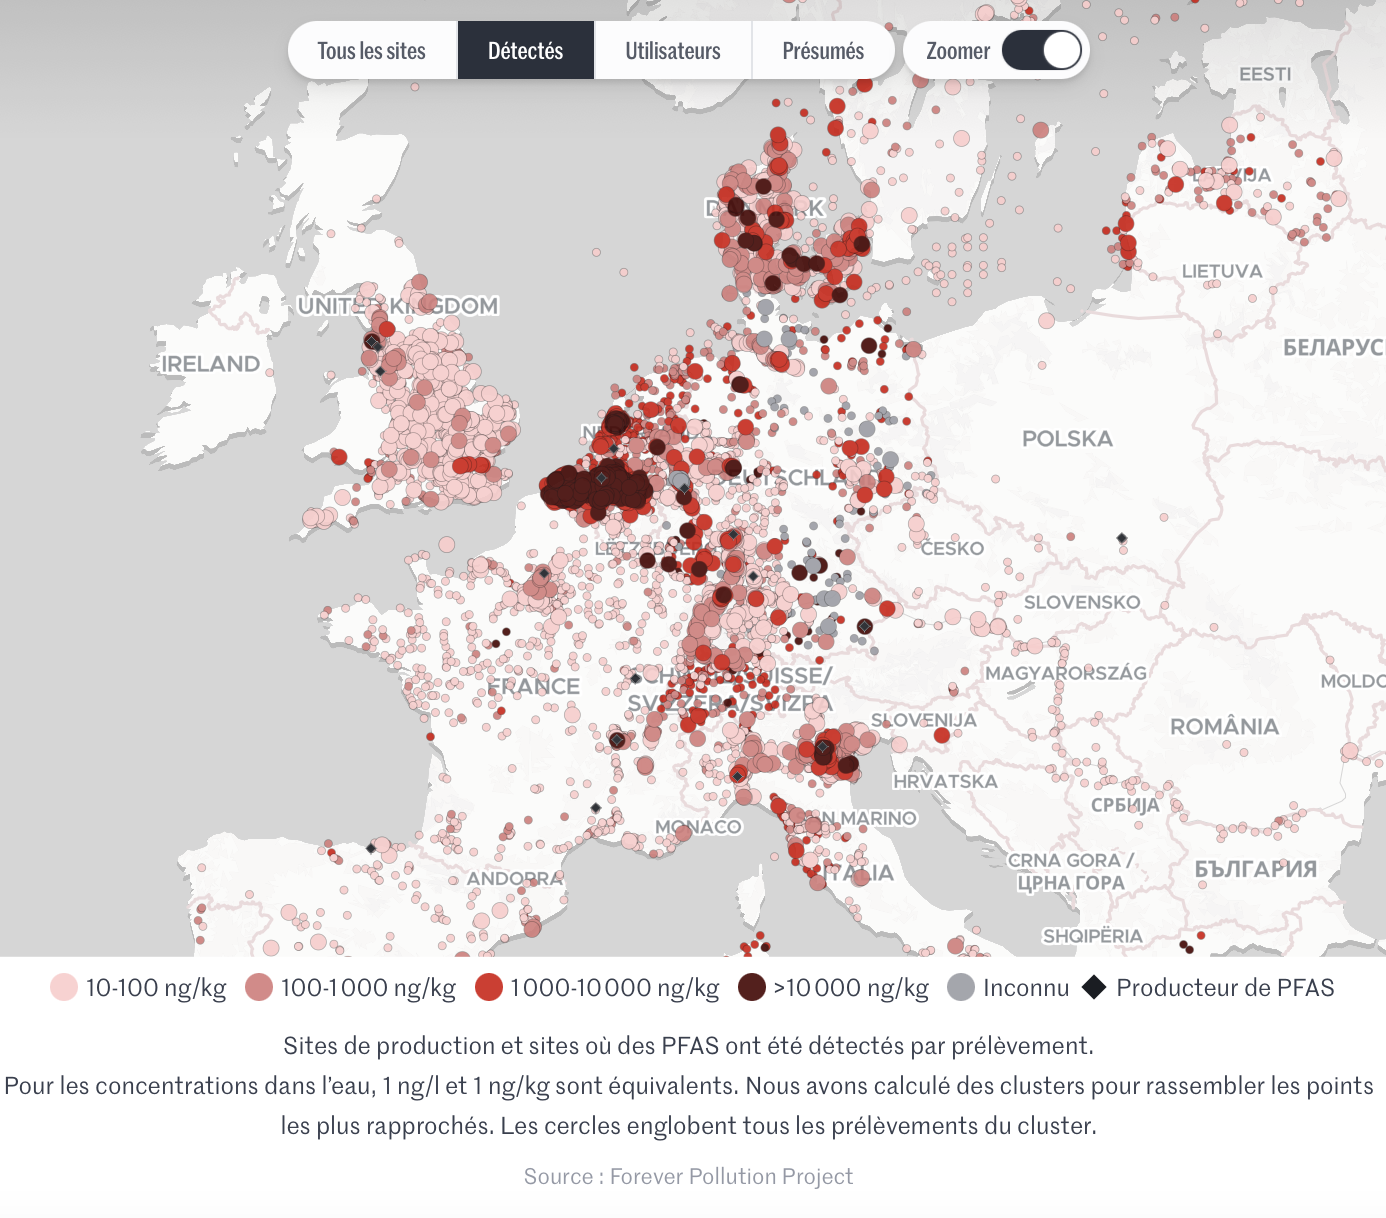
\includegraphics[width=1\textwidth]{img/intro/FPP_Carte_Clusters_SitesPFAS_Detectes.png}
\caption{Carte d'Europe des sites de détection de PFAS par prélèvements}
\label{fig:Carte_PFAS_LeMonde}
\end{figure}


% Encadré sur les PFAS

\begin{tcolorbox}[colback=gray!5!white,colframe=gray!20!white]
Le sigle \textbf{PFAS}, pour substances polyfluoralkylés et perfluoroalkylées, englobe une classe de \textbf{plusieurs milliers de substances} chimiques artificielles, inventées dans les années 1940. Antiadhésives, imperméabilisantes, résistantes aux fortes chaleurs, ces substances sont largement utilisées depuis les années 1950 dans diverses applications industrielles et produits de consommation courante : textiles, emballages alimentaires, mousses anti-incendie, gaz réfrigérants, revêtements antiadhésifs, cosmétiques, dispositifs médicaux, produits phytopharmaceutiques, etc. 

Les PFAS sont \textbf{extrêmement persistants dans l'environnement}, car la présence de liaisons carbone-fluor rend leur structure moléculaire quasi indestructible. Ils présentent de \textbf{graves risques pour la santé humaine et environnementale}. Ils \textbf{s'accumulent dans les organismes vivants}, et ne peuvent pas être éliminés. Ils sont associés à plusieurs effets néfastes sur la santé : troubles hormonaux, problèmes de développement, maladies du foie, cancers, etc. Ces molécules non éliminables et toxiques sont qualifiées de \textbf{polluants éternels}, et suscitent de sérieuses préoccupations pour la santé humaine et environnementale.
\end{tcolorbox}

La carte des points de contamination en figure \ref{fig:Carte_PFAS_LeMonde} est cohérente avec la géographie des régions industrielles françaises historiques. La majorité des points sont placés dans la moitié Nord du pays, en Île-de-France, en vallée de la Seine jusqu'à Rouen, autour de l'ancien bassin minier et sidérurgique de l'est de la Picardie jusqu'aux Ardennes. Au Sud, la vallée du Rhône se détache à partir de Lyon jusqu'à Marseille, avec Grenoble et la Savoie. Mais comparativement au reste de l'Europe, la carte de France semble clairsemée. La taille réduite des clusters de points indiquerait une concentration moyenne à faible de sites dans les régions concernées, et les concentrations relevées (en ng/kg) semblent également inférieures aux taux observés ailleurs en Europe. \\

% Forever Pollution Project - Graphique du nombre de sites recensés par pays 
\begin{figure}[!h]
\centering
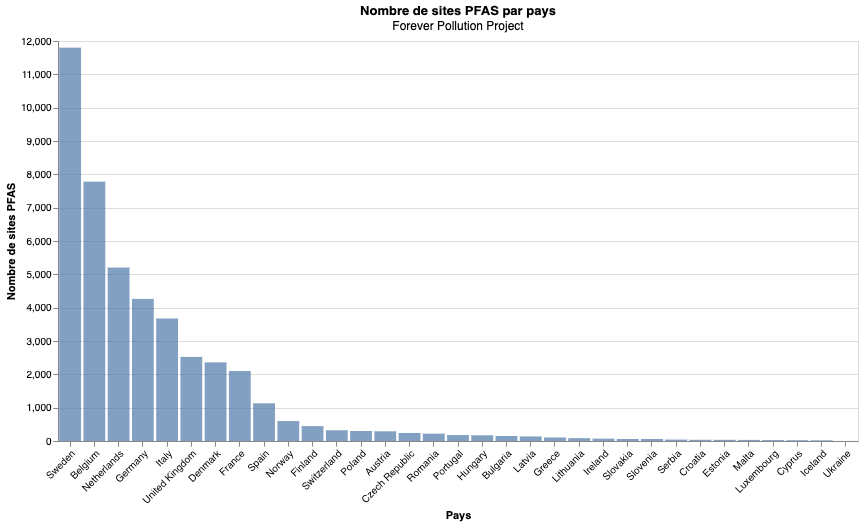
\includegraphics[width=1\textwidth]{img/intro/FPP_PFASbyEUCountry.png}
\caption{\textit{Forever Pollution Project} - Nombre de sites PFAS par pays}
\label{fig:FPP_pfas_per_country}
\end{figure}

Avec 2 100 sites recensés, soit 5\% de la base totale, le nombre de sites contaminés aux PFAS en France est en effet très inférieur à celui de ses voisins européens, et particulièrement en-deçà des données enregistrées en Suède (27\% de la base, 11 800 sites), en Belgique (17\% de la base, 7 780 sites), aux  Pays-Bas (12\% de la base, 5 203 sites) ou en Allemagne (10\% de la base, 4 263 sites). Cette grande différentiation des nombres absolus nous surprend déjà, compte tenu de l'histoire industrielle et technologique des pays concernés. Rapportés à la superficie des pays, la France aurait une densité de contamination aux PFAS beaucoup moins importante (0,003 sites par km2) que la Suède (0,026), la Belgique (0,253), les Pays-Bas (0,139), l'Allemagne (0,011) ou même Malte (0,104). La France ayant été un pays d'industrie lourde au \siecle{XX}, pourquoi la contamination aux PFAS apparaît-elle inférieure à celle de Malte ? Pourquoi la région Nord ne porte-t-elle pas une proportion cohérente de contamination aux PFAS par rapport à la Belgique ou au Luxembourg voisins, malgré son intense passé industriel ? Spatialement, les données du \textit{Forever Pollution Project} indiquent une rupture drastique de la contamination le long des frontières françaises. 

\begin{quote}
\textit{\og Our primary goal is to inform the public and to provide data to impacted community members, researchers and regulators, and to contribute to building knowledge on PFAS contamination for the public interest}" \fg{} \footnote{"Notre but premier est d'informer le public et de fournir des données aux membres des communautés impactées, aux chercheurs et régulateurs, et de contribuer à la connaissance de la pollution aux PFAS dans l'intérêt du public", \cite{horel_stephane_methodology_2023}, page 2}.  
\end{quote}

L'objectif de l'étude \textit{Forever Pollution Project} a été rempli en France, la mobilisation de l'opinion publique ayant déclenché une législation en faveur de l'interdiction des PFAS dans les objets de consommation quotidiens. La cartographie des sites contaminés et la prise de conscience de la gravité d'une contamination aux PFAS ont suffi à la faire évoluer. Bien que la situation française semble anormale dans les données, et soit probablement en-deçà de la réalité, l'étude \textit{Forever Pollution} a indéniablement ouvert une fenêtre d'opportunité politique\footnote{Voir John W. Kingdom, 1984, "Agendas, Alternatives and Public Policies", sur les fenêtres d'opportunité et les changements politiques} au sujet de la pollution endémique de l'environnement en Europe. \\

Dans le détail, les différences entres pays sont des effets de source. La méthodologie de recherche du projet est bien documentée, et suit un processus de revue par les pairs avec un appui scientifique\footnote{\footcite{horel_stephane_methodology_2023}, page 2}.  Mais les sources de données diffèrent d'un pays à l'autre. Les données du \textit{Forever Pollution Project} révèlent ainsi une géographie de la régulation de la pollution en Europe, et dessinent indirectement une arène politique et journalistique à l'échelle européenne au sujet de la reconnaissance des pollutions et de la lutte contre celles-ci.
 
% FFP France - Origine des données
\begin{figure}[!h]
\centering 
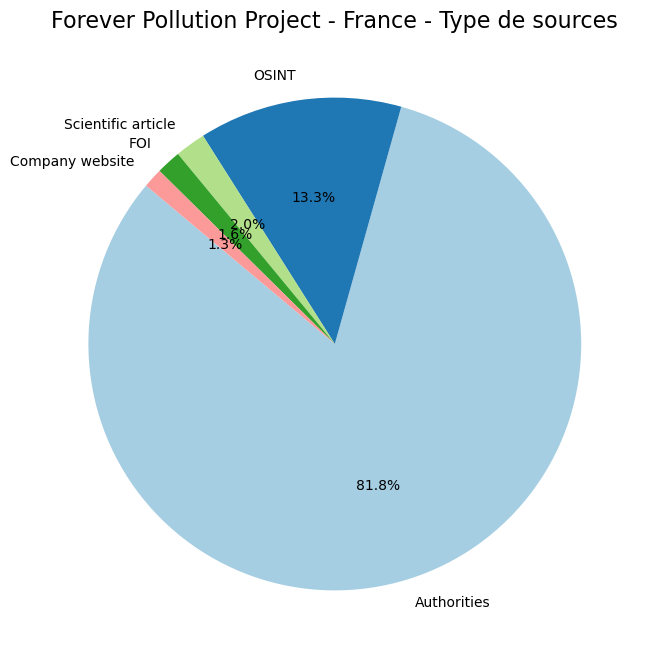
\includegraphics[width=0.3\textwidth]{img/intro/FFP_France_Type_Sources}
\includegraphics[width=0.4\textwidth]{img/intro/FFP_France_Type_Source_Autorités}
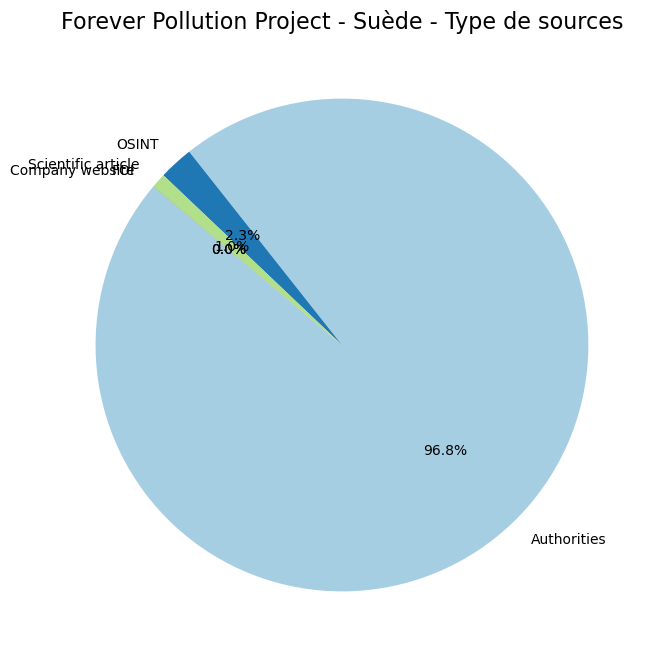
\includegraphics[width=0.3\textwidth]{img/intro/FFP_Sweden_Type_Sources}
\includegraphics[width=0.4\textwidth]{img/intro/FFP_Sweden_Type_Source_Autorités}
\caption{\textit{Forever Pollution Project} - Origine des sources, comparaison France-Suède}
\label{fig:FPP_Comparaison_Suede_France}
\end{figure}

La méthodologie du \textit{Forever Pollution Project} souligne les difficultés rencontrées par le consortium pour récolter des données sur la contamination aux PFAS, en l'absence de bases de données européenne communes sur les activités économiques et les polluants. Dans les pays les mieux documentés, la majorités des données exploitées proviennent de sources gouvernementales ou administratives. En Suède, 97\% des données sont produites par une source gouvernementale unique : la \textit{Swedish Environmental Protection Agency} (voir figure \ref{fig:FPP_Comparaison_Suede_France}). En France l'administration fournit 82\% des données, mais de quatre sources différentes, dont une extra-nationale avec l'\textit{European Environmental Agency}. Cela explique en partie la dilution des données entre la Suède et la France, en volume et en qualité. En partant d'une catégorisation d'activités connues pour leur contamination aux PFAS, les données de l'étude ont été reconstituées à partir d'une centaine de bases de données différentes. La qualité de l'information est tributaire de la qualité des données primaires, de l'objectif initial de production de ces données, et de leurs accessibilité. En France, les journalistes soulignent la difficulté d'accès aux données environnementales :  \textit{\textquotedblleft In Scotland and France, we had to wrest sampling data from the authorities using freedom of information requests \textquotedblright }\footnote{"En Ecosse et en France, nous avons arraché les données aux autorités en ayant recours à des demandes formelles d'ouverture des données" ; source : \footcite{collectif_de_journalistes_forever_2023}}. En comparaison, la Suède a inclu le suivi des PFAS dans le programme national de suivi de la pollution dès 2005. 

\begin{quote}
\textit{\og{} Our main goal was to address the disconnection between known contamination and where contamination actually is out in the world,” explain Alissa Cordner (Whitman College, Walla Walla) and Phil Brown (Northeastern University, Boston), who coordinated this work.\fg{}} \footnote{\footcite{horel_stephane_methodology_2023}}
\end{quote}

L'étude \textit{Forever Pollution Project} pose ainsi les jalons d'une géographie de la pollution en Europe, en offrant une méthodologie scientifique de traitement de données à partir de sources massives, hétérogènes (qualitatives et quantitatives) et indirectes (activités humaines). Le but du projet reste journalistique, mais en ciblant son action sur la spatialisation de la pollution, l'étude questionne un champ de recherche géographique complexe de façon très simple : si la pollution est partout, où est-elle vraiment localisée ?  \\
	
La pollution est une \og{} modification défavorable du milieu naturel qui apparaît en totalité ou en partie comme un sous-produit de l’action humaine, par des effets directs ou indirects altérant les critères de répartition des flux de l’énergie, des niveaux de radiation, de la constitution physicochimique du milieu naturel et de l’abondance des espèces vivantes \fg{} \footnote{\footcite{collectif_dictionnaire_2024}, « Pollution », p.497}. Il y a pollution d'un lieu lorsque les conditions environnementales pour la vie future y sont compromises. En ce sens, la pollution est un objet géographique socio-environnemental car elle crée de la différenciation territoriale. Elle "est" ou "n'est pas" quelque part, et l'analyse de l'ampleur d'une contamination repose sur sa spatialité : jeux d'échelles,  seuils,  diffusions, exposition. De l'étude des PFAS aux oeufs de poules, nous avons souligné qu'au \siecle{XXI} la pollution était non seulement diffuse et massive, mais éternelle. Puisqu'elle n'est pas un paramètre climatique, la pollution soulève donc la question de la chaîne de transmission des formes territoriales dans le temps. En ce sens, nous pensons la pollution comme une nouvelle dimension de la territorialité, un héritage spatial toxique transmis à travers le temps. \\

La pollution est un objet d'étude à la fois extrêmement concret, car matériel, et intangible. La pollution n'est pas toujours immédiatement visible. C'est un objet matériel dont le régime de preuve diffère car il existe d'abord à une échelle moléculaire, invisible à l’\oe{}il nu. En dehors des laboratoires, nous ne saisissons la pollution que par ses symptômes : détérioration de l'environnement, altération des cycles de vie des végétaux, des animaux, dangers pour la santé humaine. Dès lors, comment passer de la lentille du microscope à l'oeil du géographe ? Par ailleurs, comme l'illustre le \textit{Forever Pollution Project}, la pollution est également un objet politique et polémique. Son régime de preuve repose sur des données quantitatives de prélèvement qui sont l'objet de conflits autour des impacts de l'industrie sur la pollution du monde, divisant les industriels et leurs opposants (syndicats, riverains, militants écologistes, etc.). \\

Eternelle mais pas intemporelle, selon une formule de l'historien Thomas Le Roux\footnote{\footcite{le_roux_polluants_2023}}, la pollution est le produit d’une organisation socio-technique précisément située dans le temps et dans l’espace. \og{} Si la pollution est inhérente à toute activité productive (…) l’ampleur du phénomène change d’échelle avec l’entrée dans l’âge industriel \fg{}\footnote{\footcite{jarrige_contamination_2017}, p.23)} Longtemps présentée comme un mal nécessaire pour le développement humain, les travaux d’histoire de la pollution ont « dénaturalisé » la pollution en déconstruisant le discours évolutionniste et téléologique attaché à l’idée de progrès. Objets de conflits juridiques et d’oppositions dès l’installation des premières usines, les nuisances de voisinage devenues pollutions industrielles\footcite{bernhardt_demon_2002} « [définissent] l’ère de l’Anthropocène, dont l’histoire nous permet de retracer les origines comme les dynamiques sociales et politiques »\footnote{\cite{collectif_dictionnaire_2024}, \og{}Pollution\fg{}, p.497}. En étudiant les rapports de forces qui ont façonné les cycles d’industrialisation, les travaux d’histoire de la pollution retracent une autre histoire sociale et politique de la révolution industrielle, non linéaire et conflictuelle\footcite{lette_debordements_2013}. La pollution des sols appartient ainsi aux « régimes sociaux de pollution industrielle »\footnote{\cite{jarrige_contamination_2017}, p.27} qui se sont succédés dans les territoires, en particulier urbains. Les substances introduites dans les sols n’étant pas dégradables sur des échelles de temps humaines, ces héritages toxiques doivent être pris en considération en aménagement du territoire. L’étude du passé industriel d’un territoire pose ainsi plus largement la question du cycle de vie des territoires industriels et postindustriels, et de l’impact de la pollution des sols sur ceux-ci. \\

Invisible, la pollution des sols accumulée depuis au moins deux siècles percole à la surface des villes et empoisonne lentement, mais de plus en plus, les sociétés urbaines. Alors que la pollution généralisée des milieux contribue à définir l’Anthropocène comme nouvelle ère géologique\footnote{\cite{rockstrom_safe_2009} : la modification de l’occupation des sols et l’introduction de nouvelles entités dans l’environnement facteurs de pollution sont 2 des 9 limites planétaires}, l’état des sols urbains demeure un fait mal connu du point de vue des sciences sociales. Les villes sont pourtant particulièrement vulnérables à la pollution des sols, leur démographie décuplant les facteurs d’exposition, et les transformations rapides des usages du sol étant particulièrement propices à l’oubli des usages passés, même dangereux. L'impact des pollutions sur l'évolution à long terme des territoires est un champ de recherche à explorer. \\

L'étude de la pollution nous amène donc à ré-interroger nos modèles d'analyse territoriale. Notre hypothèse de départ est que la pollution industrielle des sols est un nouvel héritage spatial territorial, dont il faut tenir compte pour analyser le fonctionnement d'un espace. Nous chercherons donc à mettre la pollution au centre de la focale, afin de l'étudier en tant qu'espace. Comme pour l'étude des PFAS, nous nous heurtons à une difficulté majeure : la définition de notre corpus de données sources. Les données quantitatives étant rares, ou rarement accessibles, par quel biais aborder l'étude de substances invisibles à l'oeil nu ? En continuité avec le \textit{Forever Pollution Project}, l'utilisation des données économiques sur les activités humaines permet d'approcher une estimation des sources de pollution en un lieu et une époque donnés. Cette approche est parcellaire, car elle restreint la recherche à  un type de lieu de production et de consommation très particulier : l'usine et la zone industrielle. Le rôle de la consommation particulière des ménages est ainsi minimisé dans l'étude de la diffusion de la pollution, ainsi que le rôle du transport des substances. Nous pensons toutefois que les lieux de production industrielle demeurent les points chauds du système spatial de contamination des sols, par leur intensité productive, et par la quasi absence de régulation des émissions polluantes pendant tous les XIXe et XXe siècles. Nous nous appuierons donc sur des sources de données primaires traitant des activités industrielles. Nous dessinerons ainsi les contours du système spatial industriel en Île-de-France, pour en analyser les héritages toxiques. \\

L’organisation socio-spatiale industrielle de Paris et de sa banlieue aux XIXe, XXe et XXIe siècles\footnote{\cite{guillerme_dangereux_2004}} a produit la matérialité physico-chimique de la pollution des sols. D’un point de vue écologique, celle-ci est le résidu d’un métabolisme industriel entièrement linéarisé et externalisé\footnote{\cite{barles_ecologie_2017}} : \og{} les sociétés puisant sans cesse des ressources neuves, souvent non renouvelables, au sein de la biosphère, avant de les restituer sous une forme dégradée \fg{}. Le métabolisme d'un territoire caractérise et quantifie les flux de matières et d'énergie qui permettent son fonctionnement. Notamment développé dans les travaux d'écologie urbaine de Sabine Barles\footcite{barles_sol_1999}, ce concept nous sert de support théorique implicite pour l'étude de la pollution comme espace. Ce concept nous permet de lier la matérialité de la pollution à l'organisation socio-spatiale qui l'a produite, et de réaliser une analyse critique des dégradations environnementales. Quelle est la traduction spatiale du système industriel en Île-de-France ? Où sont localisées les poches de pollution induites? Quelles sont les bonnes échelles d’analyse de cette pollution ? Quels sont ses impacts sur les populations ? L’utilisation du concept de métabolisme territorial nous permet de définir la pollution comme une matérialité urbaine à part entière, produite par la société capitaliste industrielle et ayant des impacts sur elle en retour. Cela permet de sortir la pollution des études classiques d’économie, où elle a longtemps été caractérisée comme un simple résidu des activités économiques. \\

La transition écologique visant \og{} une profonde transformation du métabolisme territorial\footnote{Ibid} \fg{}, l’étude de la pollution des sols nous permet d’explorer les enjeux matériels de la désindustrialisation. Nous cherchons ainsi à mieux comprendre l'évolution territoriale des ancien territoires industriels, en prenant en compte la pollution des sols héritée. Le cycle de vie du foncier contraste selon les territoires. La mutation des activités semble plus rapide à Paris, où la pression foncière a transformé les fabriques en logements, en parcs ou en équipements, et où peu de friches subsistent. Dans le reste de l’Île-de-France, l’évolution des usages du sol est plus lente. La banlieue parisienne conserve des héritages industriels lourds facilement repérables dans l’espace urbain, et comptabilise la quasi totalité des 2 700 friches régionales\footnote{\cite{institut_paris_regions_observatoire_2021}}. La corrélation entre anciennes activités industrielles et état des sols y est plus importante qu’à Paris, où les terrassements et remblais successifs complexifient l’analyse causale et historique de la pollution. La question de la pollution des sols concerne ainsi aussi bien des espaces fonciers vacants que des espaces occupés, réinvestis par de nouvelles fonctions urbaines. \\

Par ailleurs, particulièrement en Île-de-France, de nouveau usages des sols se développent, liés aux aspirations des populations urbaines pour un redéploiement de la nature en ville. De nouvelles façons de faire la ville sont plébiscitées en région parisienne : végétalisation, développement des parcs et de zones favorables à la biodiversité, dés-artificialisation des sols, agriculture urbaine, « ville comestible », etc. Ces usages visant à réduire l’impact écologique des villes deviennent sensibles en cas de pollution des sols, car ils décuplent les impacts sur la santé des populations. Les poulaillers contaminés en offrent un parfait exemple, et soulignent les tensions existantes entre prise en compte de la pollution des sols urbains et développement de nouveaux usages dans le cadre de la transition écologique des villes. La renaturation de la ville sous toutes ses formes cristallise ainsi les conflits d’usages à l’œuvre dans les cycles de vie du foncier urbain, en lien avec la préservation \og{}d’une seule santé \footnote{Nous faisons ici référence au concept \textit{One Health}, « une seule santé », établissant une relation d’interdépendance dans la triade santé humaine, santé animale et santé environnementale. \cite{inrae_one_nodate}}\fg{}, humaine, animale et environnementale. \\

En somme, la pollution des sols est un vestige d’histoire urbaine comme les autres. Un héritage toxique qu'il convient de modéliser pour appréhender la pollution en tant qu'espace. Quoiqu’invisibles, ces résidus d’activités humaines non seulement nous informent sur celles-ci, mais ont aussi des impacts en retour sur les sociétés contemporaines et leurs espaces. Les pollutions sont donc à la fois des vestiges ponctuels, et un espace transmis d’une génération à l'autre. Ces vestiges de pollution ne sont plus seulement un moyen pour les sociétés de se situer par rapport au passé, ils ont une réalité spatiale dans les territoires contemporains. La création d’une mémoire de la pollution et la création de modèles spatiaux pour prendre en compte la pollution industrielle sont des étapes importantes dans la compréhension des territoires post-industriels. C'est ce que nous proposons de réaliser pour l'Île-de-France avec un focus particulier sur l'ancienne zone industrielle de la Plaine-Saint-Denis. \\

% PROBLEMATIQUE 
\textbf{Comment appréhender la pollution d’un point de vue spatial ? Quels modèles de spatialisation peut-on proposer pour prendre en compte la pollution dans l’analyse de l’évolution des villes ?} \\

Nous prendrons d'abord le temps de remettre en contexte le processus d'industrialisation en Île-de-France, à travers le destin territorial de Saint-Denis de 1810 à nos jours. Nous mettrons en évidence le double héritage industriel de Saint-Denis, entre formes urbaines en recomposition et paramètres environnementaux dégradés \textbf{(\textit{Chapitre 1})}. Puis nous soulèverons la question des sources disponibles pour étudier la pollution des sols d'un point de vue géographique. \textbf{(\textit{Chapitre 2})}. Nous présenterons ensuite notre méthodologie technique, ce qui nous permettra de reconstituer le système de lieux de la pollution industrielle en Île-de-France \textbf{(\textit{Chapitre 3})}. Enfin, en mobilisant des méthodologies d'analyse spatiale, nous formaliserons et comparerons plusieurs modélisations de l'étendue de la pollution en Île-de-France \textbf{(\textit{Chapitre 4})}.

\clearpage
\vspace*{5cm}
\hfill
\begin{minipage}{0.8\textwidth}
\begin{quotation}
% CItation non retrouvée \textit{"Le paysage d'Asnières était lugubre, une mer de béton et de briques, avec des cheminées crachant leur fumée noire et des rues étroites et sales où le vent soufflait sans fin.(...) Saint-Denis, c'était comme Asnières mais en pire. Une ville grise et triste où les gens semblaient avoir perdu tout espoir."}

\textit{ \og{} La lumière du ciel à Rancy, c'est la même qu'à Detroit, du jus de fumée qui trempe la plaine depuis Levallois. Un rebut de bâtisses tenues par des gadoues noires au sol. Les cheminées, des petites et des hautes, ça fait pareil de loin qu'au bord de la mer les gros piquets dans la vase. Là-dedans, c'est nous. \fg{} } \\

Louis-Ferdinand Céline, \textit{Voyage au bout de la nuit}
\end{quotation}
\hfill
\begin{minipage}{0.8\textwidth}
\flushright
\end{minipage}
\end{minipage}


%% CHAPITRE 1 %%
\chapter{La Plaine-Saint-Denis, héritages territoriaux de la première zone industrielle de France (de 1810 à nos jours)}
%\chapter{La Plaine-Saint-Denis, apogée et démantèlement de la première zone industrielle de France \\ (\siecle{XX - XXI})} => Ancien titre
\markboth{\MakeUppercase{\textsc{Chapitre 1}}}{}


\lettrine{L}{orsqu'en 2020,} la mairie historiquement communiste de Saint-Denis bascule en faveur des socialistes, un tournant symbolique s'opère. Communiste depuis 1944, ancien bastion ouvrier, Saint-Denis est l'exemple paradigmatique de la banlieue rouge ouvrière de petite couronne au \siecle{XX} siècle\footnote{\cite{brunet_saint-denis_1980}}. La Plaine-Saint-Denis, excroissance industrielle Sud de la ville en direction de Paris, est d'ailleurs la première zone industrielle d'Île-de-France, et de France jusqu'aux chocs pétroliers de 1972-1973. Entre le XIX et le \siecle{XX}, les usines de La Plaine ont remplacé la ceinture maraîchère de Paris. Mais ce passé communiste et ouvrier s'efface peu à peu sous les grues de chantiers de grandes ampleur. Stade de France, bureaux et équipements, universités, Grand Paris Express, sites olympiques... La pression foncière francilienne accélère la mutation de Saint-Denis depuis les années 1990.  Portant les stigmates de son passé industriel, la Plaine-Saint-Denis a fait l'objet d'aménagements et de politiques volontaristes pour relancer son développement, avec pour fer de lance la construction du Stade de France sur l'ancien site Gaz de France du Cornillon\footnote{La plus grosse usine de gaz de ville d'Île-de-France jusqu'à sa fermeture en 1965}. 

\textbf{Etudiez l'évolution urbaine de Saint-Denis, et vous aurez ainsi sous les yeux un condensé de l'histoire urbaine et industrielle de Paris et sa banlieue}. Sans réduire l'étude de l'évolution territoriale de Saint-Denis à ce seul statut, l'étude de ce destin territorial nous permet d'aborder dans ce chapitre les spécificités de l'industrialisation parisienne au XXe siècle. Si les villes offrent un miroir grossissant pour l'étude des impacts du changement climatique\footnote{\cite{barles_lurbain_2020}}, Saint-Denis offre une loupe pour l'étude des impacts à long terme des héritages toxiques d'un passé industriel sur l'évolution d'un territoire. Ces impacts forment un \textbf{double héritage spatial} à prendre en compte. Il y a d'une part les \textbf{formes urbaines} typiques d'une certaine fabrique de la ville, d'une certaine industrie lourde à Saint-Denis entre la fin du XIXe et le début du XXe siècle. Il y a d'autre part, une toxicité transmise via des \textbf{paramètres environnementaux} bouleversés par les activités humaines. La pollution industrielle est le fruit de pratiques industrielles, de façon de faire et de modes de production, combinés à la perception philosophique et pratique de l'environnement à l'époque. En retraçant l'héritage industriel de Saint-Denis, nous cherchons donc à prendre la mesure de l'héritage toxique induit. 

\section{La plaine de Saint-Denis : espaces disponibles, pollutions hors les murs (1810 - 1870)}

La pollution des milieux n'est pas l'apanage des grandes industries du début du XXe siècle. De premiers conflits environnementaux au sujet de la souillure des cours d'eau sont documentés dès le XVIIe siècle\footnote{\cite{bernhardt_demon_2002}}. Le plus souvent, il s'agit de conflit d'usage mettant en cause des artisanats polluants comme la tannerie, la brasserie, la fabrique de colle, les abattoirs, etc. Dans la fabrique des villes anciennes, le "transfert de la nuisance"\footnote{\cite{fressoz_decret_2011}} était la norme. L'activité de production et ses effets sur les milieux urbains étaient régulés par le pouvoir de police municipal, et les ateliers incommodants étaient alors bannis des centres villes\footnote{\cite{fressoz_decret_2011}}. La souillure de l'eau et les odeurs nauséabondes des traitements du cuir amenaient un rejet symbolique des tanneries en-dehors des centres urbains, ou leur circonscription à des quartiers, des rues spécifiques pour réguler leur impact sur l'environnement. 

Avant la révolution industrielle, les ateliers et les fabriques sont insérés dans le tissu urbain parisien, et sont généralement de taille modeste (une seule pièce de production). Le quartier des Halles et les faubourgs concentrent une importante activité artisanale, où la mixité des usages entre production et habitation est la norme. Cette mixité augmente même après la Révolution. Suite à la vente des biens d'Église et de noblesse, les grandes propriétés sont subdivisées en plus petites parcelles, au profit de propriétaires du Tiers Etat. Cela favorise le développement de nouvelles activités en ville. La co-présence d'activités dans un même bâtiment est courante : les cours sont partagées entre plusieurs ateliers, ou des ateliers familiaux occupent plusieurs étages d'un même immeuble. La cour de l'ancien Hôpital de la Trinité est par exemple subdivisée en plusieurs ateliers et échoppes lors de sa vente\footnote{\cite{gribaudi_ruptures_2009}}.  

Avec la révolution chimique et l'industrialisation la pollution change d'échelle, les "débordements"\footnote{au sens de conflits environnementaux des nuisances industrielles}  augmentent, et l'imbrication des lieux de vie et des lieux de production amène des conflits croissants. Entre 1804 et 1810, le changement d'échelle des pollutions industrielles par rapport aux productions artisanales "incommodantes" génère des tensions croissantes entre riverains et propriétaires d'usines\footnote{\cite{lette_debordements_2013}}. La crise de la soude artificielle de 1809-1810 engendre un changement de législation. Découvert en 1791, le procédé Leblanc permet de produire la soude artificielle à bas prix, selon un procédé nauséabond (déchets sulfurés) et extrêmement toxique (libération de chlore et acide chlorhydrique). La production de 2 tonnes de soude dégage 1 tonne d'acide chlorhydrique dans l'atmosphère, corrodant tout aux alentours. En 1809, la construction de plusieurs usines à Paris et Marseille entraîne une forte mobilisation des riverains. Le décret de 1810 "relatif aux Manufactures et Ateliers qui répandent une odeur insalubre ou incommode" est promulgué un an après le début de la crise de la soude artificielle, avec pour but de réguler ces conflits. 

Cette première régulation environnementale tranche le débat en faveur des industriels (voir chapitre 2), tout en envoyant les sources de pollution en-dehors des murs de Paris, à distance des habitations. Les travaux historiens\footnote{\cite{massard-guilbaud_genevieve_histoire_2010}} ont mis en évidence que les autorités ont très tôt eu conscience des impacts négatifs des émanations toxiques produites par les usines sur leur environnement immédiat. Le décret de 1810 correspond à une stratégie d'éloignement du problème du centre de Paris, stratégie de gestion des nuisances industrielles qui aura \textit{de jure} et \textit{de facto} un impact sur les processus d'industrialisation et d'urbanisation. \textbf{La géohistoire de la pollution en petite couronne, et particulièrement à Saint-Denis, est donc celle de l'exportation des nuisances industrielles hors des murs de Paris}. Peu accidentée, facilement accessible, agricole donc disponible à la construction, bénéficiant de vents favorables pour l'évacuation des fumées hors de la ville, la plaine de Saint-Denis offre un terrain très favorable au développement et à l'implantation des sites industriels rejetés hors de Paris. La première industrialisation de Saint-Denis se fait autour de l'industrie textile, en 1850 elle y représente 85\% des emplois industriels\footnote{\cite{adda_usine_1979}}. A la fin du \siecle{XIX}, la manufacture textile est remplacée par l'industrie lourde, l'usage de l'espace s'intensifie. C'est la naissance de la banlieue industrielle proprement dite. 

%Les implantations industrielles à La Plaine-Saint-Denis au XIXe siècle ne constituent pas encore le paysage de banlieue industrielle qui sera emblématique du développement urbain de Paris au XXe siècle. C’est au tournant de la Première Guerre Mondiale que l’accélération de l’industrialisation et la mutation du système productif développent la banlieue industrielle. 

\section{La Plaine-Saint-Denis, banlieue industrielle (1870 - 1950)}
% Puis-je parler d'apogée ici ? 
% Archétype de la banlieue industrielle
A la fin du XIXe siècle, sous l'effet de la mécanisation de l'industrie, les usines exportées hors les murs deviennent de plus en plus grandes. Ce mouvement est accentué au début du \siecle{XX} avec la Première Guerre mondiale et les prémices de la production de masse dans l'armement, la métallurgie puis la production automobile. Cette période voit également l'introduction de nouvelles méthodes de standardisation des processus de production, avec l'importation du taylorisme depuis les Etats-Unis. L'ère des chaînes de montage commence, fortement consommatrices d'espace. Ces nouvelles usines, toujours plus grandes, nécessitent de vastes zones libres pour accueillir équipements de production et infrastructures. A la recherche d'espace disponible et de main-d'oeuvre abondante, de vastes complexes industriels se développent dans les zones proches de Paris, facilitant ainsi un changement d'échelle des activités manufacturières\footnote{\cite{tabeaud_lusine_2001}}.

Phénomène amorcé à la période précédente, la localisation des industries en banlieue se généralise. L'industrialisation et la pression foncière née de l'explosion démographique de Paris\footnote{Entre 1860 et 1900, la commune de Paris passe de 1 696 000 à 2 715 000 habitants} concourent à la création d'un nouveau type de tissu urbain : la banlieue industrielle. Dans les communes limitrophes de Paris, les terrains disponibles ont favorisé l'émergence de nombreux complexes industriels. Ce nouveau paysage industriel ronge peu à peu l'ancienne ceinture maraîchère de Paris. Le Nord est de Paris est privilégié pour l'implantation des usines, une localisation "sous le vent" favorisant l'évacuation des fumées loin du centre bourgeois de la capitale. Les banlieues deviennent le théâtre d'une activité manufacturière intense, symbolisée par les cheminées d'usines et des paysages urbains noircis de résidus de combustion. 

Dans ce contexte global d'apogée industrielle en Île-de-France, \textbf{La Plaine-Saint-Denis se développe et devient l'archétype de la banlieue industrielle}. Desservie par l'axe ferroviaire Nord, l'un des plus actifs d'Europe, et par le canal de Saint-Denis inauguré en 1824 et agrandi en 1895, la commune a connu un développement industriel particulièrement intense et lourd, centré sur la métallurgie, la mécanique,  la chimie, la manufacture d'objet de consommation et quelques fabriques artistiques. Au début du \siecle{XX}, Saint-Denis compte plusieurs centaines d'établissements, au moins 300\footnote{\cite{adda_usine_1979}}, dont 17 usines métallurgiques, 29 usines chimiques, 3 verreries, une manufacture de mosaïque d'émail, l'orfèvrerie Christofle et les pianos Pleyel\footnote{\cite{musee_darcheologie_nationale_saint-denis_nodate}}. Le mouvement s'amplifie dans la suite du \siecle{XX}. En 1913, l'usine à gaz de Saint-Denis assure la moitié de la consommation quotidienne de Paris et des dizaines d'usines s'installent sur le territoire, parmi lesquelles quelques usines emblématiques comme les usines Citroën et Renault, ou la manufacture Johnson. A son apogée, la zone industrielle de La Plaine-Saint-Denis s'étale jusqu'à Aubervilliers sur près de 700 hectares, recouvrant un tiers de la surface totale des deux communes. L'industrie fournit alors un emploi à environ 50 000 personnes \footnote{\cite{adda_usine_1979}}, dont une grande partie de la population active de Saint-Denis. Face à la dureté des conditions de travail dans les usines de La Plaine, Saint-Denis "la rouge" devient le bastion de la gauche radicale ouvrière\footnote{\cite{brunet_saint-denis_1980}}. 

\section{La Plaine-Saint-Denis, de l'usine à la friche (1950 - aujourd'hui)}

%Citation article desindustrialisation
Dans les années 1950, l'Île-de-France compte 5 000 établissements industriels. La production francilienne représente environ 20\% de la production nationale, dont 50\% de la production en métallurgie et aéronautique. 38\% des actifs franciliens étaient ouvriers, soit près de 900 000 personnes. Dans les années 1960, la politique de décentralisation et la crise économique entraînent la délocalisation des entreprises installées sur le territoire. Le mouvement conduit rapidement à une désaffection de la zone industrielle. Entre 1958 et 1977, 17 000 emplois industriels sont supprimés à La Plaine-Saint-Denis, dont 14 000 sur la seule commune de Saint-Denis, dont la population ouvrière tombe dans la précarité. Entre 1972 et 1977, 2 700 emplois industriels disparaissent chaque année, partiellement compensés par le développement de l'emploi tertiaire\footnote{Date de publication de l'article \cite{adda_usine_1979}}. Les grands usines ferment les unes après les autres, au profit de délocalisations vers des pays à bas coûts de main-d'œuvre. 

\begin{figure}[!h]
\centering 
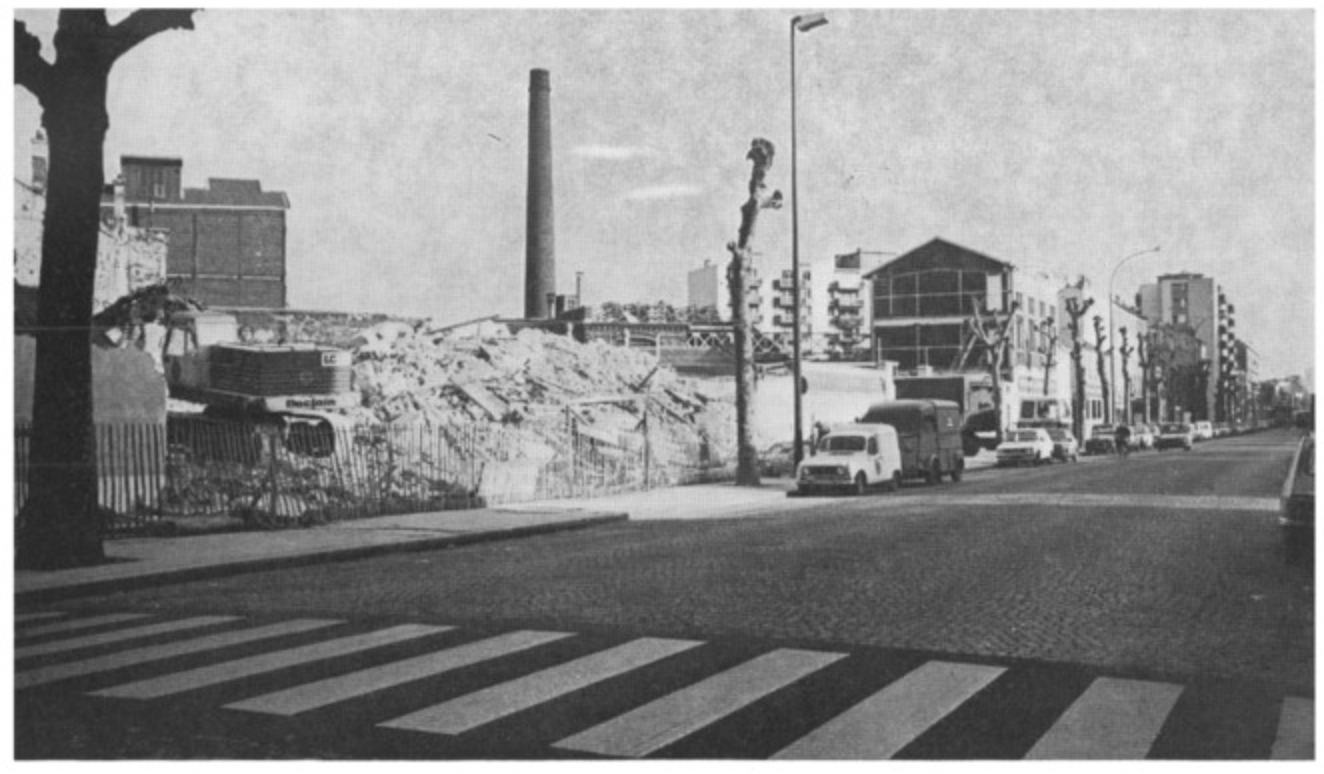
\includegraphics[width=0.75\textwidth]{img/chapitre1/Friche_STD_Photo_Etude_desindustrialisation}
\caption{Friche industrielle à La Plaine, circa 1977}
\end{figure}

Face à cette déprise très rapide de l'industrie sur vingt ans, le tissu industriel se dégrade fortement. Après l'arrêt des cheminées, de très nombreux bâtiments et terrains sont laissés à l'abandon. Les propositions de réutilisation de ces espaces sont peu nombreuses. En 1977, Serge Adda et Maurice Ducreux estiment qu'il existerait au moins 115 hectares de terrains vacants à La Plaine\footnote{\cite{adda_usine_1979}}, près de 17\% de sa surface totale. À partir de 1990, la municipalité charge une société d'économie mixte de conduire la réaffectation des friches industrielles suivant un schéma directeur qui vise à rassembler les fonctions d'habitat, de commerce et de services. En 1994, la décision d'implanter le Stade de France à Saint-Denis offre l'opportunité d'engager une première série de travaux d'infrastructure : couverture de l'autoroute A 1, déplacement et agrandissement des deux gares RER. L'objectif est de convertir la Plaine en un nouveau pôle tertiaire, sur le modèle de La Défense. 

% Extrait IAU IDF - Evolution des friches en Seine-Saint-Denis depuis les années 1990
\begin{figure}[!h]
\centering 
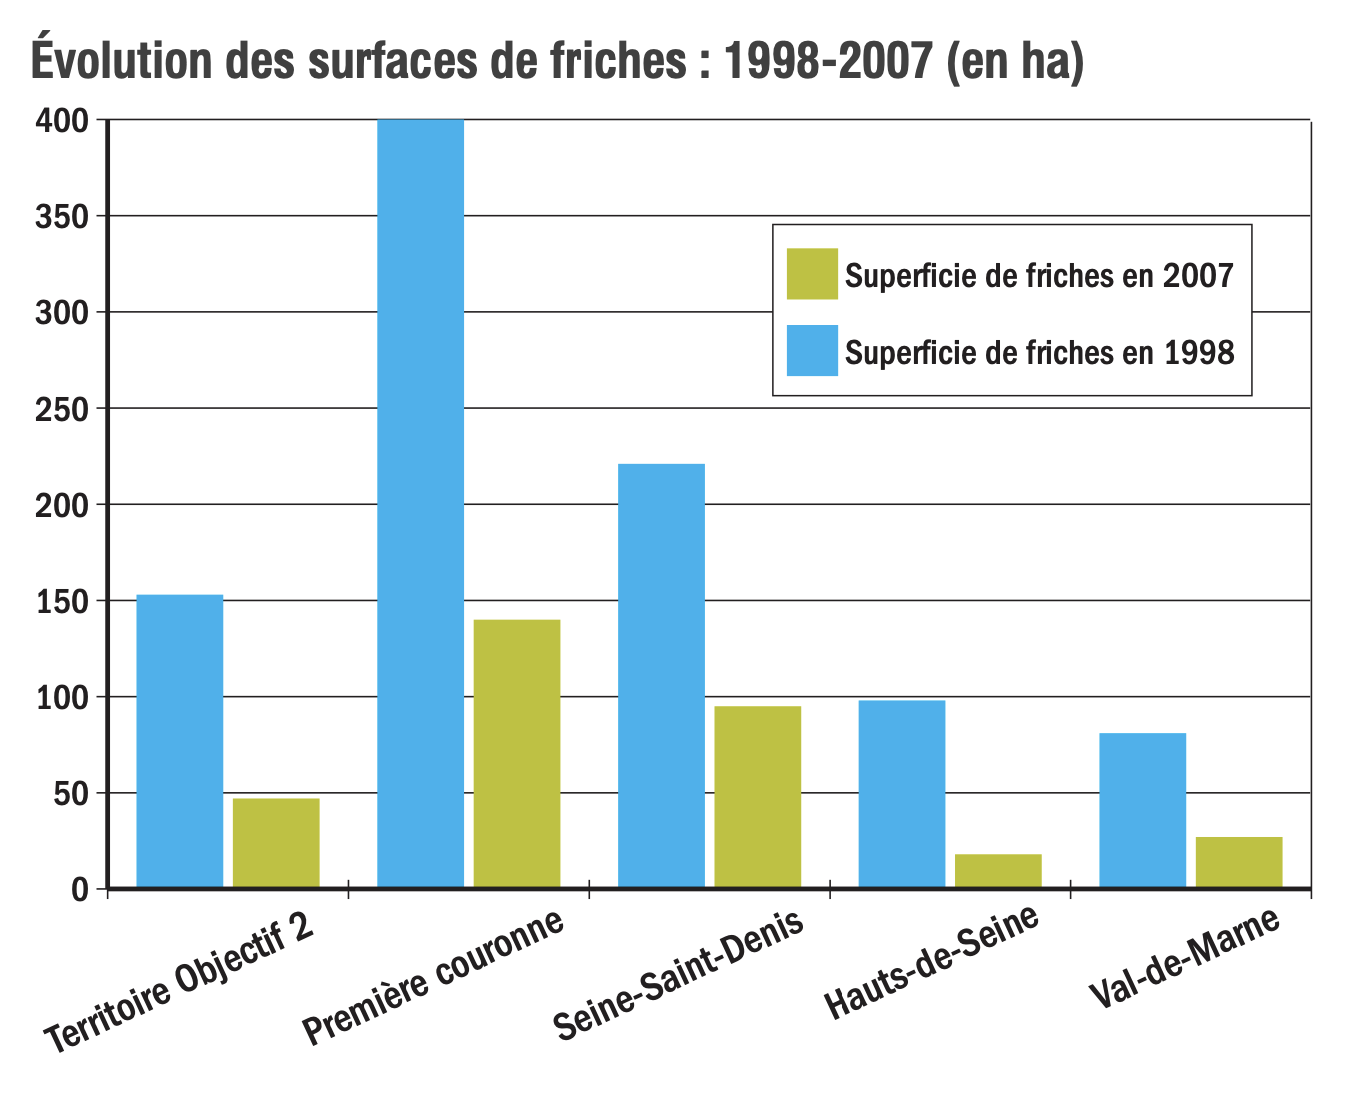
\includegraphics[width=0.45\textwidth]{img/chapitre1/IAU_NR_467_Graph_Evo_Nb_Friches.png}
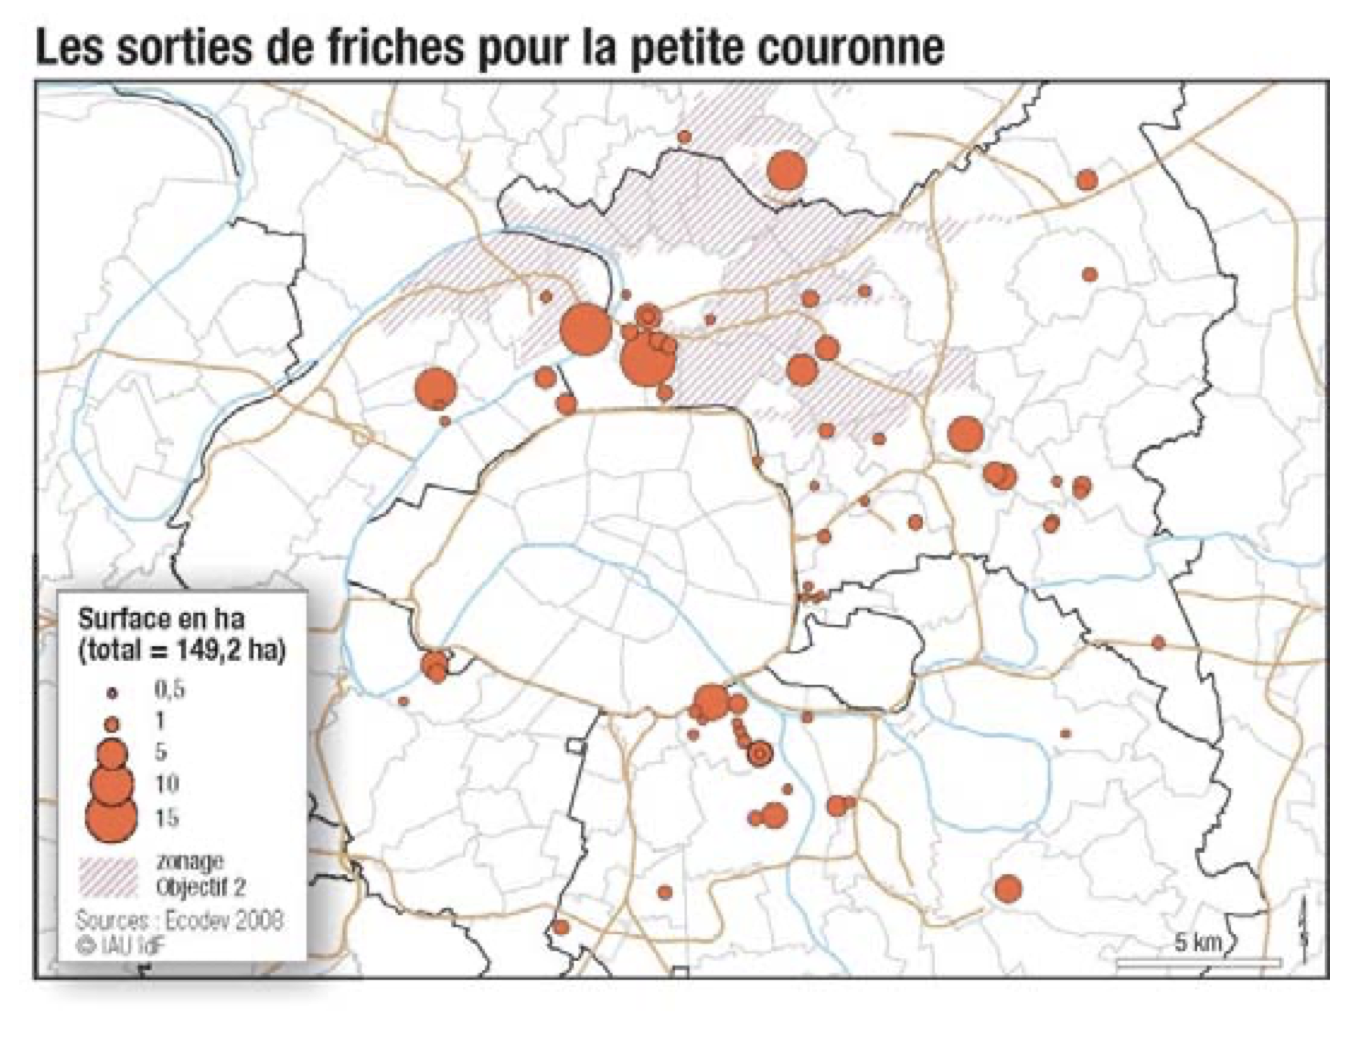
\includegraphics[width=0.45\textwidth]{img/chapitre1/IAU_NR_467_Carte_evolutionfrichesPC.png}
\caption{Source : IAU IDF, note rapide n°467, 2009}
\label{fig:IAU_Noterapide_friches_2009}
\end{figure}

Saint-Denis est aujourd'hui un territoire en plein re-développement du fait de la pression foncière. La carte des sorties de friches en petite couronne en figure \ref{fig:IAU_Noterapide_friches_2009} montre l'accélération de la réutilisation des friches entre 1998 et 2007, notamment dans le département de la Seine-Saint-Denis. Le graphique d'évolution des surfaces de friches en figure \ref{fig:IAU_Noterapide_friches_2009}\footnote{\cite{husson_jean-louis_moins_2009}} souligne quant à lui des divergences territoriales importantes entre les territoires post-industriels. En 1998, la Seine-Saint-Denis comptait pour plus de la moitié des friches de petite couronne. Si leur surface a diminué de moitié en 2007, les friches demeurent une réalité territoriale importante dans le département. Les départements des Hauts-de-Seine et du Val-de-Marne semblent avoir suivi une trajectoire urbaine post-industrielle différente de celle de la Seine-Saint-Denis. Cela témoigne de l'évolution urbaine très différente de Saint-Denis par rapport à d'autres communes post-industrielles comme Asnières ou Boulogne-Billancourt dans les Hauts-de-Seine. \footnote{\cite{ept_plaine_commune_plui_2020}, Extrait du rapport de présentation "Etat initial de l'environnement", Conseil de territoire de février 2020. Mis à jour plusieurs fois pour les projets de territoire de Plaine-Commune. Dernière mise en compatibilité en janvier 2024.} 

Si les friches urbaines sont une trace matérielle du passé industriel dans le tissu urbain, leur disparition n'efface pas la pollution infusée dans les sols et l'eau après un siècle d'industrie lourde à Saint-Denis. Les anciennes usines ont laissé un double héritage spatial : leur trace dans la trame urbaine, et la pollution dans l'environnement. Le coût exorbitant de la dépollution du site du Cornillon lors de la construction du Stade de France en témoigne.
\section{Conclusion du chapitre}

Entre le XIXe et le \siecle{XX}, l'industrie lourde française a profondément bouleversé le paysage urbain de Saint-Denis. Plaine maraîchère puis banlieue d'industrie lourde, le paysage urbain de Saint-Denis, et particulièrement de La Plaine-Saint-Denis, était dominé par les très grandes emprises industrielles et les cheminées d'usines chargées de fumées noires. Ces usines devenues friches font de Saint-Denis un territoire post-industriel en pleine recomposition, aux prises avec un héritage socio-spatial complexe. Nous avons ainsi voulu nous donner des clés de lecture historiquement informées des processus d'urbanisation et d'industrialisation en Île-de-France, pour mieux comprendre l'héritage territorial d'une ancienne banlieue industrielle. 

Cet héritage territorial est aussi un héritage toxique. L'industrialisme triomphant a favorisé une pollution décomplexée et endémique typique de la période. Frédéric Ogé\footnote{\cite{oge_sites_2004}, page 19} cite par exemple ce propose tenu en 1832 lors du creusement du puit de Bondy : \og{} On peut envoyer sans crainte dans le sol les matières les plus infectes \fg{}. Les scientifiques en charge du projet étaient alors persuadés que les substances retourneraient à l’état de poussière dans l'environnement, le déversement dans l'environnement les rendant au cycle des matières. Sous les anciennes usines, l'héritage spatial du tissu urbain se double d'un héritage toxique déposé sous le sol des anciennes usines. Si les cheminées arrêtent de fumer, la pollution des sols, des sous-sols et des eaux demeure bien en place. Ces traces environnementales du passé industriel constituent une dimension spatiale à part entière des territoires industriels et post-industriels.

\textbf{L'héritage industriel de Saint-Denis combine ainsi une forme spatiale, l'usine et la zone industrielle, et une toxicité, la pollution des sols et de l'eau.} En comprenant l'histoire industrielle de Saint-Denis, et son héritage territorial, nous cherchons ainsi à délimiter le régime spatial industriel spécifique de Saint-Denis, dont est dépositaire le territoire actuel. Nous proposons donc d’ajouter une échelle territoriale supplémentaire au système spatial industriel, en considérant le systèmes des lieux de l’industrie comme un système de lieux de pollution. Si le système industriel francilien s’est désagrégé, en particulier à Saint-Denis, le système de pollution hérité demeure en place dans l’environnement. C’est ce système de lieux de pollution que nous nous proposons d’étudier à présent, en le reconstituant à partir des sources historiques sur les risques industriels. 

%Sous les anciennes usines, quel est l'état de la pollution des sols ?
%%%%%%%%%%%%%%%%%%%%%%%%%%%%%%%%%%%%%%%%%%%%%%%%%%%%%%%%%%%%%%%%%%%%%%%%%%%%%
%% CHAPITRE 2 %%
\chapter{La pollution et ses sources : la mémoire environnementale des lieux d’industrie}
\markboth{\MakeUppercase{\textsc{Chapitre 2. La pollution et ses sources}}}{}

\lettrine{S}{i} l'histoire sociale, politique et économique de Saint-Denis l'ouvrière bénéficie d'une documentation importante et a fait l'objet de nombreux travaux d'historiens, il n'en va pas de même de sa géographie environnementale. Quelles sont les sources disponibles sur l'état des sols, de l'air et de l'eau à la Plaine-Saint-Denis, et dans le reste de l'Îe-de-France ? Sur quelles données pouvons-nous nous appuyer pour étudier la pollution des sols d'un point de vue géographique ? Comment reconstituer la réalité spatiale de la pollution, en limitant les effets de source ?

Nous avons cherché à mettre la pollution au centre de la focale, à nous décentrer. Mais dès lors, quelles sources utiliser ? Sous quel angle ? Nous verrons dans ce chapitre qu'en nous concentrant sur les traces des activités humaines passées, nous nous sommes placée dans la lignée de travaux d'histoire environnementale et de sociologie de l'action pour nourrir nos travaux sur la géographie environnementale de la pollution industrielle.  

\section[Les sources sur la pollution des sols]{Les sources sur la pollution des sols}

\textbf{La cartographie des sources disponibles révèle la grande complexité d'accès aux données sur la pollution en France, particulièrement celle des sols. Les données existantes sont éparses, de qualité inégale, et non exhaustives}. Au début de notre recherche, nous avons rapidement constaté la grande dispersion des acteurs et institutions impliqués dans le recensement et la gestion des données sur la pollution de l'environnement. La grande diversité de polluants à prendre en compte fut une autre difficulté pour la construction de notre corpus de recherche. Notre premier axe de recherche étant la pollution industrielle dans le département de la Seine-Saint-Denis, nous avons réalisé une exploration des sources disponibles à ce sujet, en élargissant à toute l'Île-de-France. La première étape de notre travail de recherche fut donc de réaliser une cartographie de l'état des sources. 

La pollution des sols est un sujet très politique éminemment lié à la valeur du foncier. Si l'on trouve relativement facilement des données sur la pollution atmosphérique, et dans une moindre mesure sur l'eau, on trouve difficilement en accès libre les sources permettant de proposer des estimations de niveaux de pollution des sols. A titre de comparaison, en Île-de-France, les données sur la qualité de l'air sont diffusées en temps réel par Airparif. Quant à l'eau, si l'ensemble des données ne sont pas publiques, le système d'information sur l'eau (SIE) rassemble les données à l'échelle nationale depuis 2003. Aucun système équivalent de mesure et d'archivage n'existe concernant l'état des sols, sujet qui fut longtemps une affaire économique plutôt que de santé publique. Le bureau de géologie nationale, initialement nommé Bureau de Recherches Géologiques et Minières (BRGM), avait pour mission de mettre la géologie nationale au service de la prospection minière. L'eau et l'air corrompus ayant des impacts délétères rapides sur la santé humaine, ils firent rapidement l'objet d'études sanitaires dédiées, ouvrant la voie à l'hygiénisme urbain\footnote{Citons par exemple les études du Dr John Snow à Londres sur l'épidémie de choléra en 1854}. La pollution des sols se caractérise le plus souvent par une exposition prolongée à des doses plus réduites. La législation française de régulation de la pollution reflète ce déséquilibre apparent des sources. Depuis 1961 pour la pollution atmosphérique\footnote{Loi du 2 août 1961 relative à la lutte contre les pollutions atmosphériques et les odeurs}, 1964 pour l'eau\footnote{Loi du 16 décembre 1964 relative au régime et à la répartition des eaux et à la lutte contre leur pollution}, des cadres juridiques existent pour en surveiller la pollution. Des normes d'émission et des seuils de pollution ont ainsi été inscrits dans la loi, nécessitant de fait la création d'appareils techniques de mesures pour en assurer la régulation. Un tel système centralisé n'existe pas encore pour la mesure de la pollution des sols. Ce qui s'en approche le plus relève de la gouvernance de l'activité industrielle.  
 
En réalisant notre cartographie des sources sur la pollution des sols, nous avons ainsi identifié plus de dix-sept jeux de données de qualités et de périmètres inégaux. Parmi ces données, nous trouvons la mention de données quantitatives, des bases de données rassemblant les mesures de la pollution conduites sur le terrain. L'une d'entre elles, la base de données sur les sols urbains (BD SolU) appartient d'ailleurs à un projet national de création d'une base de données sur la pollution des sols \footnote{Voir le site internet BDSolU : \url{https://www.bdsolu.fr/fr}}. Il semble néanmoins qu'à date cette entreprise ait peu avancé depuis la fin du premier projet expérimental en 2021. Les données quantitatives sur la qualité des sols sont ainsi inaccessibles au public et introuvables en ligne. Nos demandes de contact sont demeurées sans réponse dans les délais impartis pour notre mémoire. Par ailleurs, selon les quelques descriptions trouvées en ligne, ces données quantitatives existantes ne sont pas exhaustives. Il s'agit de points de mesure où des prélèvements de sols sont effectués ponctuellement. A l'heure où nous écrivons ces lignes, il n'existe pas en France de politique systématique de mesure de la pollution des sols afin de créer un point de comparaison quantitatif unifié sur le territoire. Ce n'est par exemple pas le cas en Belgique ou en Suisse, où une étude de pollution est obligatoire avant tout acte d'achat immobilier ou foncier.

Nous trouvons en revanche un nombre important de bases de données qualitatives, intéressantes à exploiter dans le cadre de notre étude. Ces données qualitatives, pour celles qui sont diffusées, sont des données produites par l'Etat français, relevant pour la plupart de la gestion du risque industriel. Ce sont ces données administratives qui s'avèrent les plus complètes pour notre étude, du point de vue de l'homogénéité de l'information et de la mise en qualité. Ces données sont le fruit de la législation française pour la régulation du risque industriel. En effet, s'il n'existe pas encore de législation sur l'état des sols en tant que telle, il existe de très longue date en France une régulation du risque industriel à l'échelle nationale. Ce sont ces données que nous allons exploiter, après un bref rappel sur l'histoire de la régulation du risque industriel en France. En utilisant ces données, nous avons donc étudié la pollution des sols du point de vue de l'héritage toxique produit par les activités humaines successives. 

\section[De la nuisance au risque]{De la nuisance au risque : évolution de la perception du risque industriel en France}

Toute donnée est le produit de processus sociaux et historiques. C'est ce que met en évidence Alain Desrosières dans \textit{La Politique des grands nombres} au sujet des statistiques publiques, et cette théorie s'applique plus largement à tous les efforts de quantification du monde social. Alain Desrosières analyse la manière dont le développement des statistiques contribue à la formation de l'Etat moderne. De la même façon, le développement de la régulation des affaires environnementales par l'Etat est allé de pair avec l'émergence de données sur la pollution des sols. Il s'agit alors de construire 

\vspace{1em}
\begin{quote}
\og un espace de commune mesure, à l'intérieur duquel les choses sont comparables, parce que les catégories et les procédures de codage sont identiques. Ce travail de standardisation du territoire a été une des tâches essentielles de la Révolution française de 1789, avec le système unifié des poids et mesures, le découpage des départements, la création de l'état civil laïc, et le Code civil \fg{} \footnote{\cite{desrosieres_politique_2010}, page 17}
\end{quote}
\vspace{1em}


En un sens, ces données administratives que nous exploitons pour étudier la pollution appartiennent à des "procédures matérielles d'objectivation"\footnote{\cite{desrosieres_politique_2010}, page 34} du phénomène industriel, mises en place par l'Etat dès le début du XIXe siècle pour réguler les conflits environnementaux liés à l'industrialisation. Nous ébaucherons dans cette sous-partie le contexte socio-politique d'émergence et de production des données publiques sur la pollution des sols. Nous verrons que la définition du risque industriel a beaucoup évolué, et qu'un changement de paradigme s'est opéré avec la prise de conscience de la crise environnementale dans les années 1970. 

\subsection{1810. "Dangereux, insalubres, incommodes"\thanks{\cite{guillerme_dangereux_2004}, Le titre de l'ouvrage est une référence à la loi de 1810} : naissance de la régulation du risque industriel en France}

Il important de noter qu'en France les données sur la pollution des sols se confondent en partie avec celles sur la régulation du risque industriel. La régulation du risque industriel constitue la première forme de régulation environnementale développée en France dès le début du \siecle{XIX}. En 1810, l’une des premières législations environnementales en France concerne la régulation de ce que l’on appelle alors les nuisances industrielles. Les premiers conflits environnementaux prennent la forme de conflits de voisinage, où les riverains se mobilisent contre l’implantation d’usines à proximité des lieux d’habitation\footnote{\cite{jarrige_contamination_2017}}. En 1810, la politique impériale de régulation des établissements \og{} dangereux, insalubres, incommodes\fg{} reprend l’ordonnance de 1806 de la préfecture de police de Paris qui obligeait les exploitants à déclarer leurs activités. A cette époque, seules les nuisances au voisinage sont prises en compte, la notion de pollution n’existe pas dans son acception contemporaine\footnote{\cite{bernhardt_demon_2002}}. L'historien Jean-Baptiste Fressoz démontre dans ses travaux, que cette première législation environnementale "libéralise les choses environnantes", favorisant \textit{de facto} les entreprises industrielles au détriment des riverains. \footnote{\cite{fressoz_decret_2011}}. 

\begin{quote}«En 1810, le but fondamental du décret est de protéger le capital industriel contre les récriminations des voisins. L’ancien ministre de l’Intérieur Jean-Antoine Chaptal, un des inspirateurs du décret, qui était un des plus grands industriels chimistes de son temps (un des plus grands pollueurs, aussi), souhaitait avant tout stabiliser l’acte d’entreprendre en dégageant l’industriel des incertitudes produites par la police » (page17) 
\end{quote} 
Le décret de 1810 inaugure une régulation environnementale financière basée sur le principe du pollueur payeur. Cette dernière laisse de fait le champ libre à l'industrialisation et à l'accélération de la pollution de l'environnement. Il ouvre également la voie à l'accentuation des inégalités spatiales liées aux impacts toxiques de l'industrialisation. 
\vspace{1em} 
\begin{quote}"Le principe de compensation des dommages combiné à l’impératif de rentabilité économique produisait trois résultats : l’emploi (pour les tâches les plus dangereuses) des populations les plus faibles, dont les maux pouvaient rester invisibles ; la concentration de la production et de la pollution dans quelques localités ; enfin, le choix, pour ces localités, des territoires pauvres, dépourvus des ressources sociales et politiques augmentant la valeur de la compensation environnementale."\footnote{\cite{fressoz_decret_2011}, page 21}. 
\end{quote}
\vspace{1em}
Les premières données de pollution sont par conséquent des pièces d'archives juridiques et législatives, qui dessinent un espace juridique de confrontation entre riverains et industriels. Ce sont donc d'abord des données qualitatives qui sont produites, contrairement aux statistiques publiques qui occupent Alain Desrosières. La création des bases de données contemporaines sur la pollution sont en grande partie un recensement des traces juridiques laissées par la première législation sur le risque industriel en 1810 : autorisations d'implantation d'usines, conflits juridiques, etc. A l'orée du \siecle{XIX}, la nécessité de comptabiliser les impacts de l'industrie sur l'environnement est occultée par l'idéologie de progrès diffusée dans la société par les tenants du libéralisme\footnote{\cite{jarrige_contamination_2017}}. 

La législation sur le risque industriel se développe au rythme des accidents industriels, et à la suite des mouvements de mobilisation contre l’industrie qu'ils engendrent. L’un des premiers accidents industriels d’ampleur documenté en région parisienne est l’explosion de la poudrerie de Grenelle en 1794, où 1000 personnes trouvent la mort\footnote{\cite{ministere_de_lenvironnement_explosion_2006}}. Cependant, quoique cet accident déclenche à Paris un surcroît de recours au pouvoir de police, menant \textit{in fine} au décret de 1810, la question du risque industriel est occulté pendant une large part du \siecle{XIX}. L'hygiénisme opère le "basculement des étiologies de l'environnement vers le social"\footnote{\cite{fressoz_decret_2011}, page 21}, et les usines deviennent des symboles de prospérité et de progrès sanitaires. Un tournant s'opère dans la définition du risque industriel dans les années 1970, suite à la crise de Seveso.

\subsection{1976. Crise de Seveso et émergence de la question environnementale en Europe}

La législation sur le risque industriel se développe au rythme des accidents industriels qui émaillent la deuxième moitié du \siecle{XX}, compromettant gravement la santé et la sécurité des populations, et à la suite des mouvements de mobilisation sociale qu'ils engendrent. Le 10 juillet 1976, l’explosion d’une usine dans la petite ville de Seveso dans la banlieue de Milan, contamine 37 000 personnes et près de 20 000 hectares de sols, décimant animaux et végétaux aux alentours\footnote{\cite{combe_catastrophe_2020}}. De la dioxine TCDD (2,3,7,8-tétrachlorodibenzo-p-dioxine) est relâchée en très grande quantité dans l’environnement. Cet accident de très grande ampleur choque l’ensemble de l’Europe et déclenche une mobilisation internationale en faveur d'une régulation plus stricte des sites industriels dangereux. La directive SEVESO de l’UE est votée en 1982, donnant une nouvelle base juridique pour l’encadrement des industries au sein de l'Union Européenne. 

\vspace{1em} 
\begin{figure}[!h]
\centering 
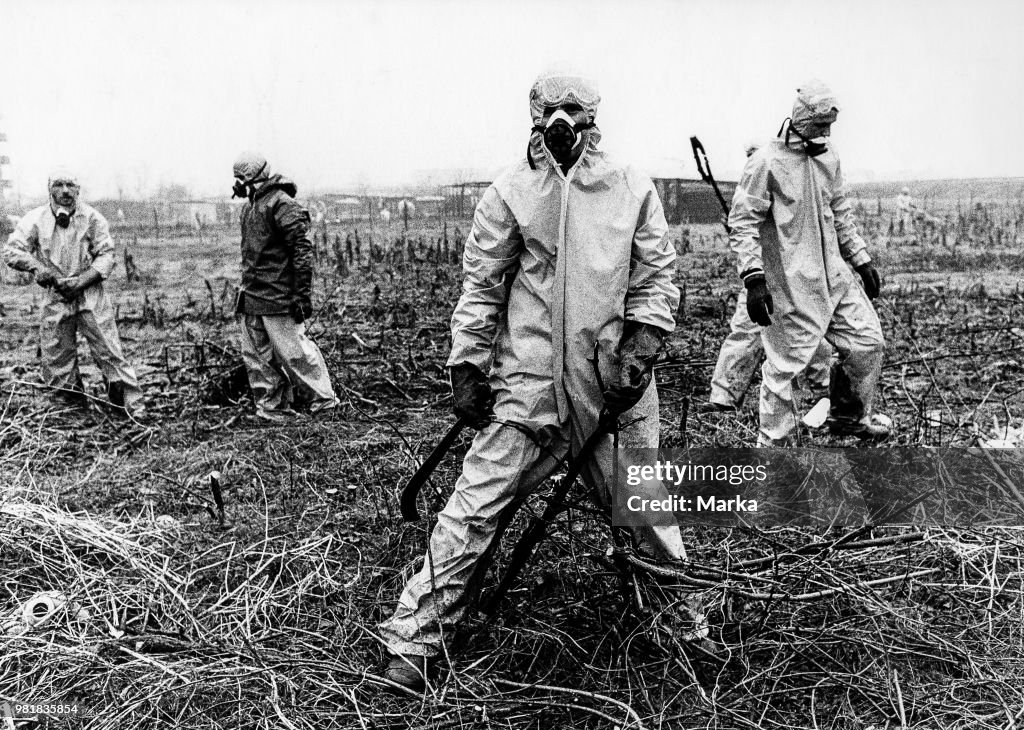
\includegraphics[width=0.75\textwidth]{img/chapitre2/SEVESO1976}
\caption{Photo prise pendant la crise de Seveso en 1976}
\end{figure}\footnote{Source : Getty Images}

En réponse au scandale Seveso et face aux préoccupations croissantes de la population au sujet des risques posés par l'industrie, le gouvernement Chirac promulgue le 19 juillet 1976 la loi sur les installations classées pour la protection de l'environnement (ICPE) et signe le décret d'application le 02 février 1977. Cette législation crée la première brique d'un appareil d'Etat de gestion du risque industriel. La loi ICPE prévoit une "approche intégrée"\footnote{\cite{ineris_historique_nodate}} du risque industriel, c'est-à-dire un guichet administratif unique pour le suivi des sites industriels. C'est la création de l’inspection des installations classées\footnote{Voir la loi de 1976 sur les installations classées}. Et puisque pour gouverner il faut connaître ce que l'on doit administrer, cette loi débouche en 1978 sur le premier recensement des sites pollués en France\footnote{\cite{brgm_casias_nodate}}. Ce recensement vise à identifier les "sites ICPE" relevant de la nouvelle norme de contrôle des risques et susceptibles de provoquer des pollutions. Cet inventaire ICPE initial a posé les bases des efforts ultérieurs pour une gestion plus systématique des sites pollués. Le rapport Lacaze commandé par le ministère de l'Environnement en 1985 sur les friches industrielles relance la politique de recensement des sites douteux\footnote{\cite{oge_sites_2004}, page 9}. L'impact négatif du passé industriel sur les possibilités de réutilisation des sols est déjà un problème bien identifié. 
\begin{quote}
“Les contaminants du sol peuvent réduire à néant un reverdissement, une réutilisation agricole ou jardinière. Les plantes peuvent elles-mêmes transférer la toxicité vers la chaîne alimentaire.”\footnote{\cite{oge_sites_2004}}
\end{quote}
Cela aboutit en 1988 au lancement d'une nouvelle campagne de recensement des sites industriels pollués par le ministère de l'Environnement. L'objectif du recensement de 1988 est d'identifier de manière exhaustive les sites et sols contaminés nécessitant une intervention des pouvoirs publics pour assurer leur réhabilitation. Les résultats de ce recensement permettent de dresser une cartographie plus précise de la pollution industrielle en France. Ce recensement jette les fondations d'une approche plus proactive de l'Etat en matière de surveillance et de gestion des sites pollués, conduisant à la création de la base de données des sites et sols pollués (BASOL) en 1994. BASOL recense les sites et sols pollués ou potentiellement pollués qui nécessitent une action des pouvoirs publics, soit sous forme de surveillance, soit sous forme de travaux de dépollution. Elle est destinée à fournir des informations sur la nature des pollutions, les actions entreprises et l'état d'avancement des travaux de réhabilitation. La base de données des anciens sites industriels (BASIAS) rassemble les anciens sites industriels ne faisant pas l'objet d'un suivi dans BASOL. 

% Inclure un schéma ou un encadré sur les bases de données ?  

A partir de 1988, les autorités publiques se trouvent ainsi en possession d'informations (littéralement) explosives. Le volume de sites pollués découvert dépasse les prévisions initiales, un "Verdun chimique"\footnote{\cite{oge_sites_2004}, page 7} offrant matière à un scandale national. C'est ce que sous-entend Frédéric Ogé dans son ouvrage de 2002 \textit{Sites pollués en France: enquête sur un scandale sanitaire}. Cet ingénieur CNRS révèle l'étendue de la pollution des sols auprès du grand public. Il dénonce la minimisation de la pollution par l'administration, et le flou juridique quant au traitement des sols pollués. Alors qu'en 2002 l'Etat annonçait 900 sites contaminés dans toute la France, Frédéric Ogé explique que la base de données BASOL recense déjà plusieurs milliers de sites, dont 2 900 à Paris et 7 000 en petite couronne. 

Le débat publique déclenché par l'ouvrage de Frédéric Ogé est suivi de peu par une nouvelle catastrophe industrielle mortelle, déclenchant un nouveau renforcement de la législation du risque industriel. Le 21 septembre 2001, l'usine Azote Fertilisants (AZF, filiale de Total) à Toulouse explose suite à une réaction chimique de nitrate d'ammonium dans son entrepôt (une substance hautement explosive et sensible aux chocs). 31 personnes trouvent la mort, 2500 sont blessées, et les quartiers alentours sont endommagés sur plusieurs kilomètres. L'usine AZF était un établissement ICPE classé, mettant ainsi à jour les lacunes du système de contrôle des sites mis en place en 1978. L'accident génère une grande préoccupation quant à la sécurité effective des sites ICPE. La loi ICPE est renforcée en 2003 avec l'adoption de la loi sur la prévention des risques technologiques et naturels majeurs. Cette loi renforce les mesures de prévention et les contrôles. Elle met également en place un régime de sanctions en cas de non respect des normes. La loi encadre l’urbanisation à proximité des installations déclarées à hauts risques, et met en place des plan de prévention des risques technologiques, les PPRT.           

 \vspace{1em} 
\begin{figure}[!h]
\centering 
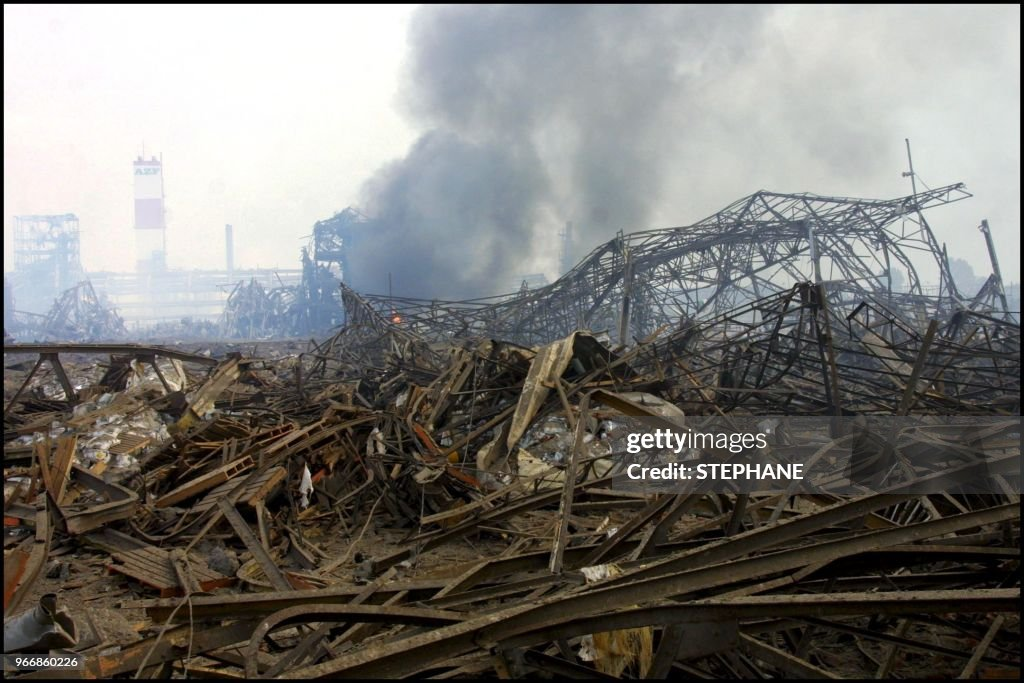
\includegraphics[width=0.75\textwidth]{img/chapitre2/explositionAZF.jpeg}
\caption{Photo des dégâts causés par l'explosion de l'usine AZF en 2001}
\end{figure}\footnote{Sources : Getty Images}

% Ajouter ici le tableau de synthèse des dates : accidents / législation / production de données (page 46 cahier bleu)?

\subsection{1994. Émergence d'une mémoire environnementale du risque industriel} 

Les controverses et la réticence politique à diffuser les données sur l'état des sols révèlent la relation complexe entre connaissance de l'état des sols et politiques de remédiation. Les données administratives disponibles sur la pollution des sols, les bases de données ICPE, BASOL et BASIAS, sont ainsi le produit de la politique de gestion du risque industriel, et la production de ces données relie science et action tel que décrit par Alain Desrosières dans son travail d'anthropologie des sciences statistiques. Les données sur la pollution des sols sont ainsi prises dans une dialectique complexe entre description scientifique et décision politique prescriptive\footnote{\cite{desrosieres_politique_2010}, page 13}. Il est quasiment impossible d'entamer une estimation de la pollution des sols sans utiliser ces bases de données publiques. Ces données qualitatives ne nous offrent donc que le point de vue du régulateur. 

\begin{quote}
Mais justement parce que le domaine d'étude [la statistique] est un lieu d'interaction entre les mondes du savoir et du pouvoir, de la description et de la décision, du "il y a" et du "il faut", il se trouve avoir déjà, préalablement à la recherche, un rapport particulier à l'histoire"\footnote{\cite{desrosieres_politique_2010}, page 10} 
\end{quote}
Les données sur le risque industriel nous offrent néanmoins une nouvelle perspective d'étude sur les héritages territoriaux toxiques de la pollution industrielle, grâce à 15 ans de travail historique en archives. De 1994 à 2020, sous la tutelle du ministère de l'Environnement, des inventaires historiques régionaux (IHR) sont financés par l'Etat français dans chaque département afin de recenser l'ensemble des activités industrielles et de services passées. L’objectif est de reconstituer une « mémoire environnementale » des anciennes activités industrielles, émettrices de pollutions, pour suivre l’évolution des usages des sols après la désindustrialisation. Au lancement de ces campagnes systématiques de recensement, 150 ans d'histoire industrielle nationale sont à documenter. Les données recueillies dans le cadre de ces inventaires sont archivées dans la base de données nationale BASIAS déjà existante, qui deviendra la Carte des Anciens Sites Industriels et Activités de Services (CASIAS) en 2020\footnote{\cite{brgm_casias_nodate}}. La base CASIAS est pilotée à l'échelon départemental pour le compte de l'Etat central (ministère de l'Environnement). Elle fait le fruit de campagnes d'archives régulières jusqu'en 2020 pour la constituer. Elle continue à être mise à jour en continu, nécessitant l'extraction des données en tenant compte de la date. Nous reverrons cela dans le chapitre suivant, où nous détaillerons notre chaîne de traitement.

L’objectif de la base de données BASIAS / CASIAS est de constituer une « mémoire environnementale » des anciennes activités industrielles, potentiellement émettrices de pollution, afin de documenter l’évolution des usages des sols après la désindustrialisation, et d'orienter la stratégie nationale de gestion des sites et sols pollués. 
\begin{quote}
\textit{La circulaire du Ministère du 3 décembre 1993 a défini la politique française de traitement et de réhabilitation des sites et sols pollués autour de trois axes d’actions : recenser, sélectionner, traiter. A la demande du Ministère, le BRGM a entrepris, dès 1994, la réalisation de l’inventaire des anciens sites industriels et activités de service, demande formalisée par une lettre de mission en date du 16 avril 1999. Cet inventaire répond à trois objectifs principaux (cf. Arrêté du 10-12-1998 et Circulaire du 26 avril 1999 adressée aux préfets) :
\begin{itemize}
\item recenser, de façon large et systématique, tous les sites industriels abandonnés ou non, susceptibles d’engendrer une pollution de l’environnement,
\item conserver la mémoire de ces sites,
\item fournir des informations utiles aux acteurs de l’urbanisme, du foncier et de la protection de l’environnement.
\end{itemize}
A cet effet, les informations recueillies dans le cadre de l’inventaire ont été stockés dans la base de données BASIAS}.\footnote{\cite{brgm_casias_nodate}}. 
\end{quote}

Devant l'ampleur des phénomènes de pollution, la stratégie nationale est de dépolluer selon les usages des sols. Dès lors, la constitution d'une mémoire environnementale est essentielle. Cette démarche de constitution d'une mémoire environnementale a été conduite de façon systématique sur le territoire. Le concept de mémoire environnementale a d'abord été employé en biologique au sujet de la persistance d'une information au sein d'un système environnemental au sujet d'un événement ou d'une modification antérieure. Ces archives environnementales font églement référence au phénomène cognitif générationnel du "shifting baseline syndrome"\footnote{\cite{pauly_anecdotes_1995}}. Cela correspond à la réévaluation générationnelle de l'étalon de biodiversité servant à évaluer la réduction de la diversité du vivant. En somme : pour la génération ayant grandi dans les années 1970, le "silent spring" décrit par Rachel Carson correspond à une expérience de biodiversité maximum\footnote{\cite{carson_silent_1962}}. 

\vspace{1em} 
\begin{figure}[!h]
\centering 
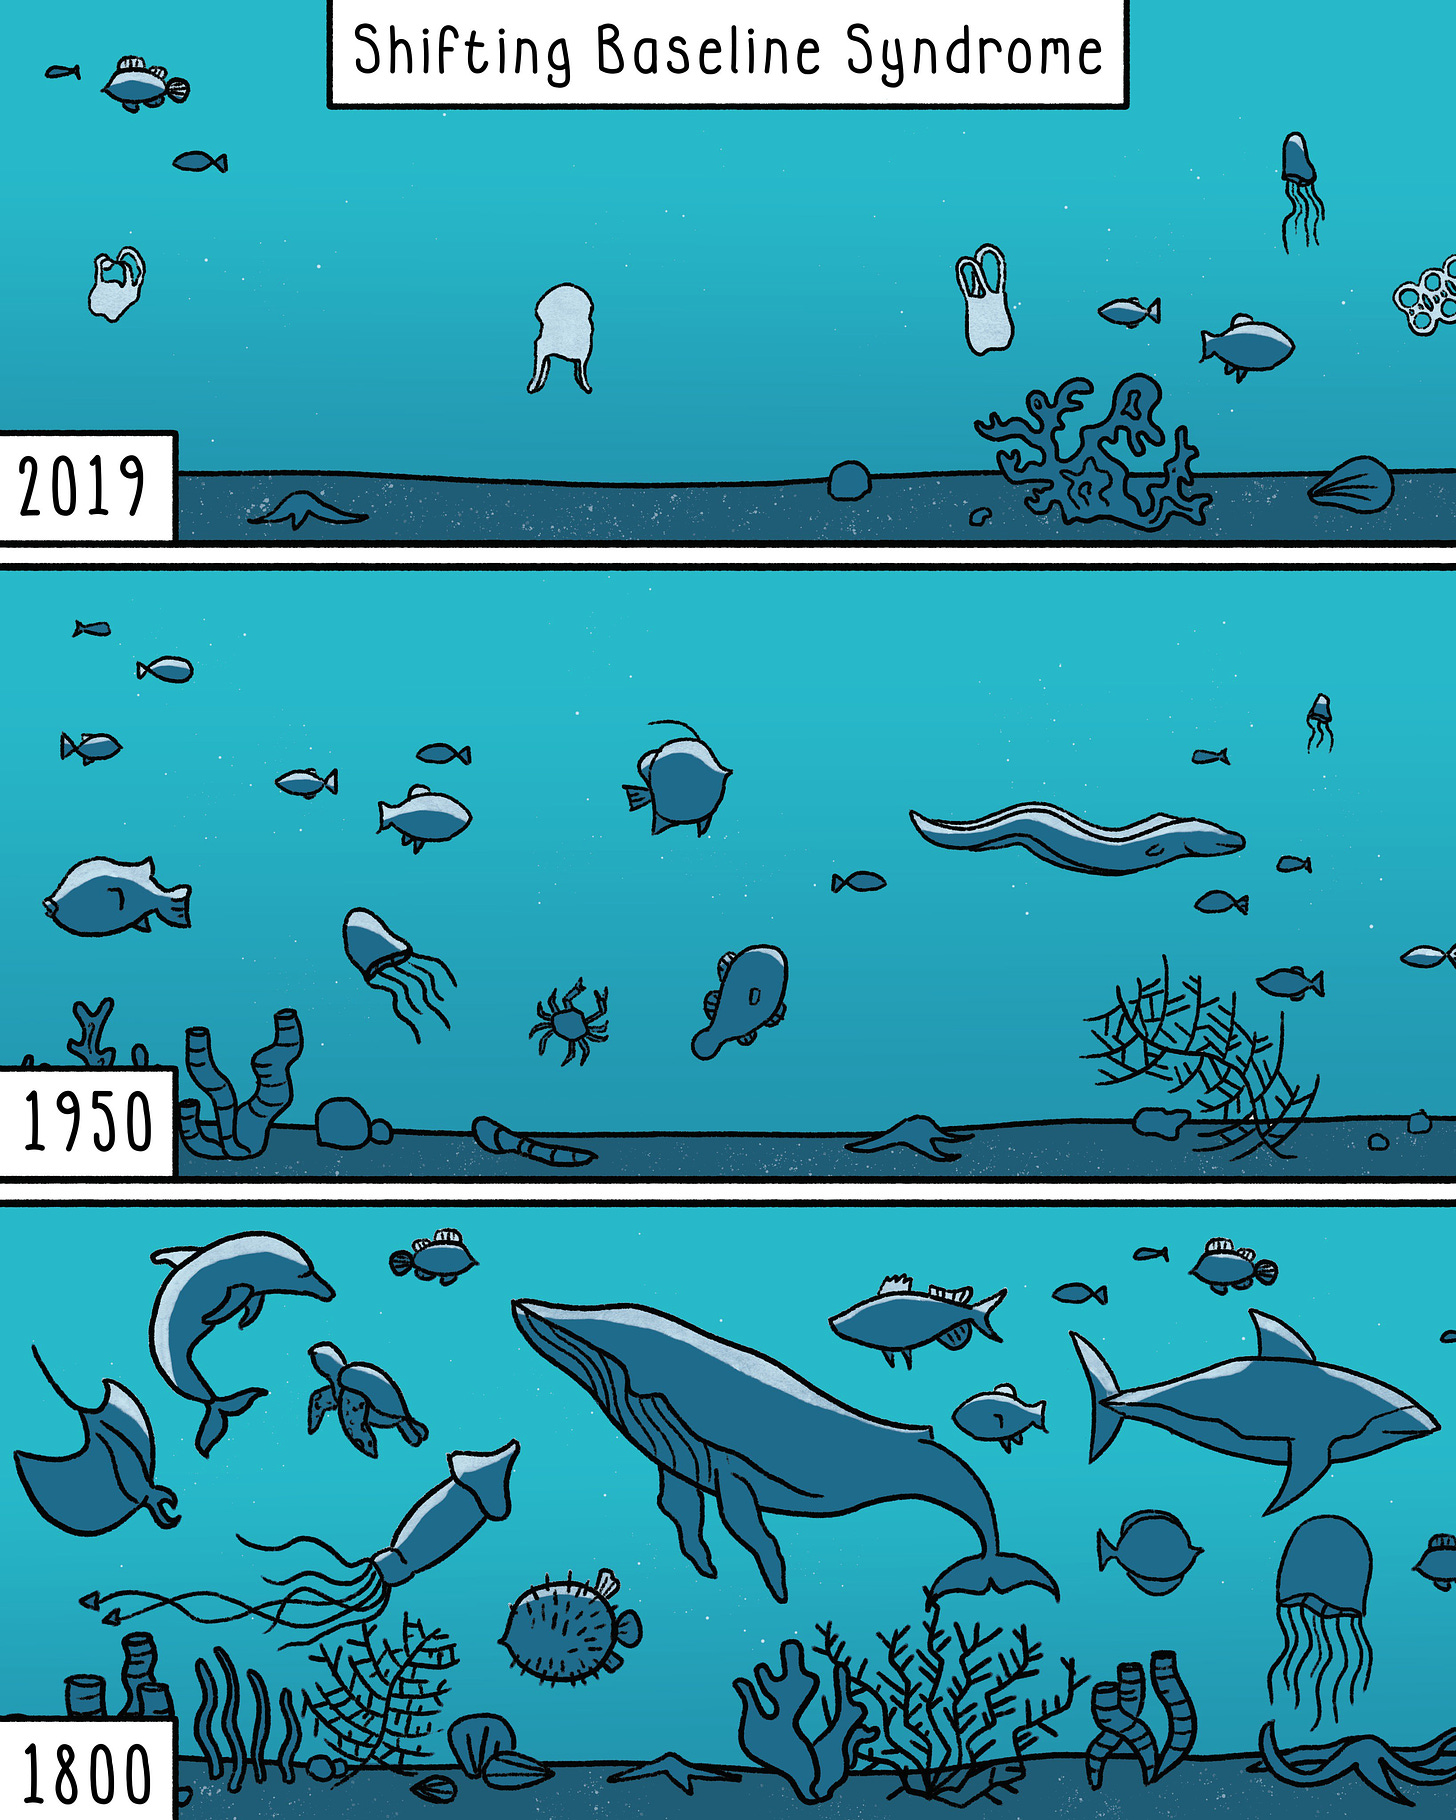
\includegraphics[width=0.75\textwidth]{img/chapitre2/shifting_baseline_syndrome.jpeg}
\caption{Illustration du shifting baseline syndrome}
\end{figure}\footnote{Source : post Twitter/X du 24/01/2021 du compte Biodiversityloss (@BiodiversitySOS)}

Avec la prise de conscience des impacts des risques technologiques sur les populations et l’environnement, la nécessité de conserver la mémoire des anciennes activités tenues en un lieu est devenue une évidence. Ainsi, miroir de la prise de conscience environnementale opérée dans l'opinion publique et en politique, la création des bases de données sur le risque industriel ont opéré une "procédure matérielle d'objectivation"\footnote{\cite{desrosieres_politique_2010}, page 34} de ses héritages toxiques potentiels. Ces données nous offrent bel et bien une nouvelle perspective sur l'histoire de l'industrialisation, environnementale et géographique. La pollution des sols se définit ainsi comme un espace de risques, un espace administratif et juridique de régulation et de suivi des activités industrielles. Son contrôle par l’État souverain appartient au pouvoir régalien sur le sol et le sous-sol. La pollution est ainsi constituée d’une multitude d’espaces ponctuels, attachés à la parcelle, régis par le régime de la propriété, où l’État souverain peut se substituer aux propriétaires défaillants, au titre des activités qui y ont été ou y sont menées. Par le biais du suivi des activités conduites sur un territoire, ce sont bien les excipients polluants qui sont examinés, et c’est un système de lieux de pollution qui émerge. La pollution est, par le biais du suivi des activités industriels, un espace administratif et juridique de calculs des risques technologiques. 


\section{Conclusion du chapitre}

La construction d'un corpus scientifiquement probant pour analyser spatialement la pollution des sols en Île-de-France s'est heurtée à la dispersion et à la mauvaise qualité des données disponibles. Nous avons donc concentré notre étude sur les données les plus homogènes à l'échelle régionale : les données de gestion du risque industriel, et plus particulièrement la base de données CASIAS. Fruit d'un travail en archive de longue haleine, cette base de données concentre donc notre étude sur les espaces productifs industriels, occultant ainsi les lieux de transports, et de consommation des matières polluantes. Si nous reprenons l'exemple du \textit{Forever Pollution Project}, les lieux de consommation de PFAS sont partiellement pris en compte (les casernes de pompiers et les aérodromes pour les mousses de dispersion anti-incendie par exemple). Là où le \textit{Forever Pollution Project} inclut lieux de pollution présumée et lieux de pollution avérée, la base de données CASIAS est une base de données qualitative, qui ne nous permettra de travailler qu'avec des hypothèses de pollution. Nous nous appuyons donc sur des lieux d'histoire industrielle pour en inférer une histoire environnementale, et une géographie de la pollution industrielle. 

Dans ce chapitre, la question des sources disponibles sur la pollution des sols nous a amené à considérer la genèse d'un appareil d'Etat d'enregistrement et d'encodage statistique des faits environnementaux. En prenant pour référence les travaux d'Alain Desrosières, nous avons vu comment le développement de ces données environnementales participe à la constitution d'un "espace cognitif d'équivalence et de comparabilité, construit à des fins pratiques"\footnote{\cite{desrosieres_politique_2010}, page 399}. En reprenant le cadre d'analyse que celui-ci propose pour les statistiques publiques, la base de données CASIAS que nous allons exploiter dans le chapitre suivant constitue un "outillage distinct", "politico-administratif" : un "système d'enregistrement, de codage, de tabulation"\footnote{\cite{desrosieres_politique_2010}, page 399} du monde socio-environnemental. %La comparaison avec l'objet d'étude de Desrosières s'arrête là, quoique la base de données CASIAS devienne un objet statistique par dénombrement. 

Les accidents industriels ont rythmé la prise de conscience environnementale, et ouvert un espace de débat européen au sujet de la pollution industrielle. La politisation croissante de l'accidentologie industrielle au \siecle{XX} fait passer la pollution du statut d'externalité économique négative à celui de responsabilité socio-environnementale des entreprises et de l'Etat. Le développement de la gestion du risque industriel contemporain participe donc à un mouvement plus large de dé-naturalisation de la pollution\footnote{Mouvement inverse à la "naturalisation" de la pollution étudiée par Thomas Le Roux et François Jarrige dans \cite{jarrige_contamination_2017}}. La constitution des bases de données nationales sur le risque industriel correspond à un tournant majeur dans l'espace d'information environnemental \footnote{Voir \cite{desrosieres_politique_2010}, page 405, sur la transformation de l'espace d'information économique}. Les données administratives CASIAS dessinent un espace cognitif de référence sur les anciennes activités industrielles et leurs héritages toxiques potentiels. Cet espace cognitif commun, nous le nommons mémoire environnementale. A partir de cette mémoire environnementale, nous proposerons des modèles de spatialisation de la pollution industrielle potentielle en Île-de-France dans la suite de notre étude. 

Nous traçons ici les contours d'une géographie environnementale basée sur l'étude des actions humaines et de leur spatialisation. Ces données qualitatives nous donnent une perception de l'espace industriel cumulé en Île-de-France, mais n'est pas encore une reconstitution diachronique de l'évolution des paysages industriels. Nous réaliserons ainsi une analyse de la pollution d'un point de vue cumulatif, par ailleurs cohérent du point de vue de l'accumulation des substances dans l'environnement. Nous dessinons ainsi les contours de ces héritages toxiques accumulés sous les usines. 

%%%%%%%%%%%%%%%%%%%% CHAPITRE 3 %%%%%%%%%%%%%%%%%%%%%%%%%%%%%%%%%%%
\chapter{Le système de lieux de la pollution industrielle à Saint-Denis et en Île-de-France}
\markboth{\MakeUppercase{\textsc{Chapitre 3. Le système de lieux de la pollution industrielle}}}{}

\lettrine{L'}{industrialisation} en Île-de-France est un processus socio-historique et un système spatial, dont les anciennes usines listées dans CASIAS sont les lieux d'histoire. Dans une perspective d'analyse spatiale, un lieu est une 

\begin{quote}
"unité spatiale élémentaire, dont la position est à la fois repérable dans uns système de coordonnées et dépendante des relations avec d'autres lieux dans le cadre d'interactions spatiales"\footnote{\cite{clerc_lieu_2004}, d'après Béguin(1979)}
\end{quote} 

Les données CASIAS dessinent ainsi autant de "sous-ensembles de l'espace"\footnote{\cite{grataloup_christian_introduction_2023}, page 61} industriel francilien. Leur mobilisation nous permet de passer de l'administration du risque industriel à la modélisation de l'impact environnemental de l'industrie, prenant ainsi en compte ce que nous considérons comme une nouvelle dimension inéluctable de la territorialité. Au-delà du lieu comme point géocodé, c'est donc un système spatial, et une forme de géographicité de l'industrie en Île-de-France que nous cherchons à découvrir\footnote{\cite{clerc_lieu_2004}}.

Dans ce chapitre, ainsi que l'exige tout travail en Humanités Numériques, nous prendrons d'abord le temps de décrire rigoureusement nos données source et notre chaîne de traitement. Puis nous exploiterons l'étape dite d'exploration des données pour mettre en évidence le système de lieux de la pollution industrielle en Île-de-France. 

\section[Chaîne de traitement Python sur CASIAS]{Croiser CASIAS et ActiviPoll : reconstituer le système des lieux de la pollution industrielle en Île-de-France }

\subsection{La base de données CASIAS}
La \textbf{Carte des Anciens Sites Industriels et d'Activités de Services \mbox{(CASIAS)}} recense les anciennes activités humaines sur l'ensemble du territoire national. Depuis 2021 elle reprend les sites industriels autrefois répertoriés dans la base de données BASIAS, qui n'avait jamais été publiée auparavant. Très exhaustive, elle se révèle particulièrement intéressante pour retracer l'histoire des activités industrielles d'avant 1973, date de création par l'INSEE de la base de données SIRENE sur les entreprises. Tout comme la base SIRENE, CASIAS est mise à jour en continu par l'administration. Elle est mise à disposition en open data sur la plateforme Géorisques\footnote{Page de téléchargement des données : \url{https://www.georisques.gouv.fr/donnees/bases-de-donnees/inventaire-historique-de-sites-industriels-et-activites-de-service}}, le portail national d'information sur les risques naturels et technologiques\footnote{Si les données sur le risque industriel ont bel et bien été mises à disposition du public via la plateforme Géorisques, conformément à l'article 173 de la loi ALUR de 2014, force est de constater que leur accessibilité n'est pas facilitée. La documentation est fort peu développée. Il est peu aisé pour le néophyte de s'orienter dans cette masse de données.}. 

Chaque ligne de la base de données CASIAS représente un point dans l'espace, chacun correspondant à une ancienne activité industrielle, sa description et sa localisation (exprimée en degrés pseudo-Mercator, en projection WGS 84). Comme l'illustre le tableau des variables ci-dessous, chaque site recensé possède un identifiant unique Sites et Sols Pollués (SSP), un code technique le reliant à sa campagne d'inventaire régional. Dans le meilleur des cas, le nom de l'établissement et son adresse sont indiqués avec la géolocalisation précise. Les adresses récupérées lors des campagnes d'archives ont été géocodées par l'administration. 

% Capture CSV avant traitement
\begin{figure}[!h]
\centering 
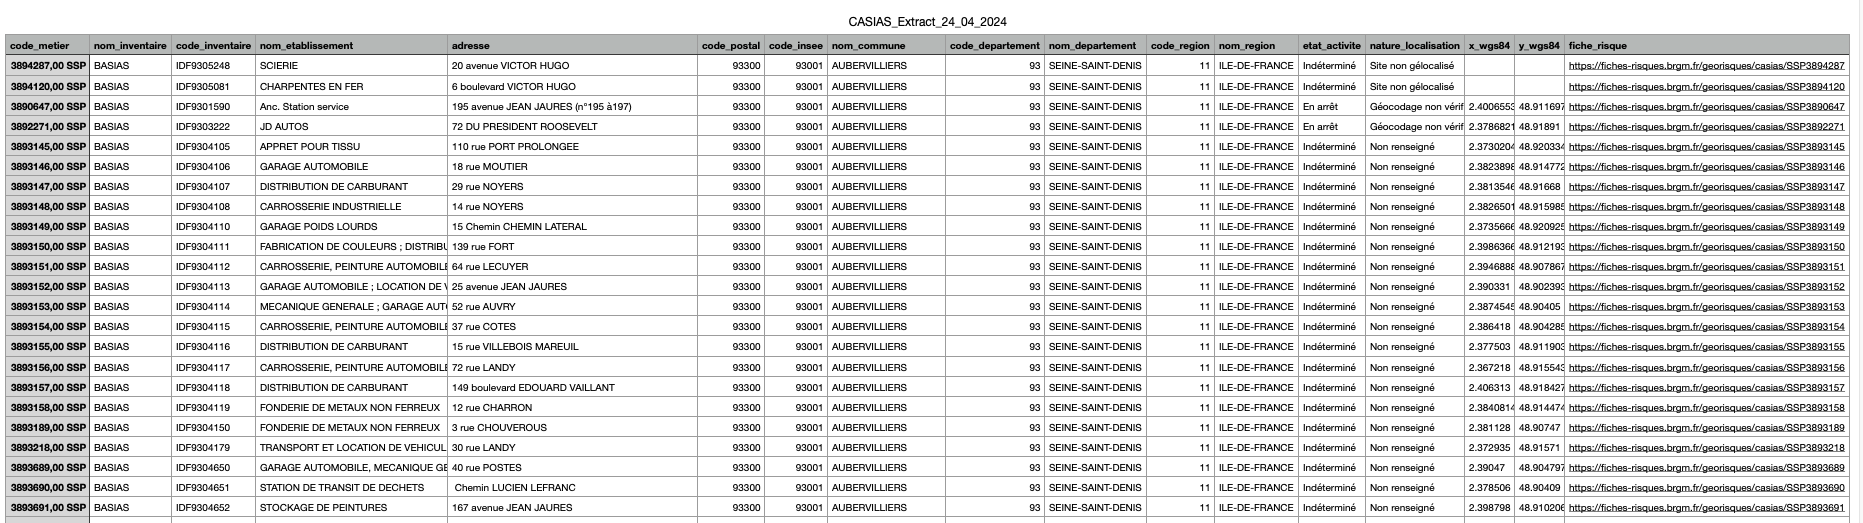
\includegraphics[width=1\textwidth]{img/chapitre3/CASIAS_Capture_Tableau_Initial.png}
\caption{Structure des données CASIAS, Extrait du tableau avant traitements}
\label{fig:casias_donnees_brutes}
\end{figure}

% Table de description des variables
\begin{table}[h]
\centering
\small
\caption{Description des variables de CASIAS}
\begin{tabular}{>{\raggedright}p{3.5cm}p{9cm}}
    \toprule
    Variable & Contenu \\
    \midrule
    code\_metier & Code unique Sites et Sols Pollués ssp  \\
    nom\_inventaire & Référence à la BDD d'inventaire \\
    code\_inventaire & Code unique d'inventaire régional \\
    nom\_etablissement & Nom du site, si retrouvé en archives \\
    adresse & Adresse de l'ancien site \\
    code\_postal & Echelles géographiques \\
    code\_insee & Echelles géographiques\\
    nom\_commune & Echelles géographiques \\
    code\_departement & Echelles géographiques \\
    nom\_department & Echelles géographiques \\
    code\_region & Echelles géographiques \\
    nom\_region & Echelles géographiques \\
    etat\_activite & Etat de fonctionnement du site, si connu \\
    nature\_localisation & Evaluation du géocodage \\
    x\_wgs84 & Longitude en degrés  \\
    ywgs84 & Latitude en degrés \\
    fiche\_risque & Lien vers la fiche risque CASIAS complète \\
    \bottomrule
\end{tabular}
\end{table}

Chaque ligne du tableau correspond à une fiche risque établie par l'administration centrale, accessible via une adresse url figurant en dernière variable. Les données du tableau sont un extrait réduit de cette fiche. Les données attachées à chaque point sont en réalité bien plus riches que celles listées dans le tableau. En conséquence, nous avons dû coder en python une chaîne de traitement pour récupérer les informations dont nous avions besoin pour notre étude (voir sous-partie 3.1.3). Pour la région Île-de-France, nous récupérons ainsi le \textbf{22 avril 2024}, date de notre dernière extraction de données pour ce mémoire\footnote{CASIAS étant mise à jour en continu par l'administration, il est important de réaliser toute récupération d'informations dans un délai court après l'extraction des données. Nous avons donc dû repartir sur une nouvelle extraction de la base de donnée fin avril, pour diminuer le taux d'échec de notre webscrapping.}, \textbf{36 738 points uniques référencés dans CASIAS}, sachant que ce résultat est probablement en-deçà de la réalité du nombre d'industries et activités humaines ayant existé dans la région depuis le \siecle{XIX}.

% Capture fiche risque web 1
\begin{figure}[!h]
\centering 
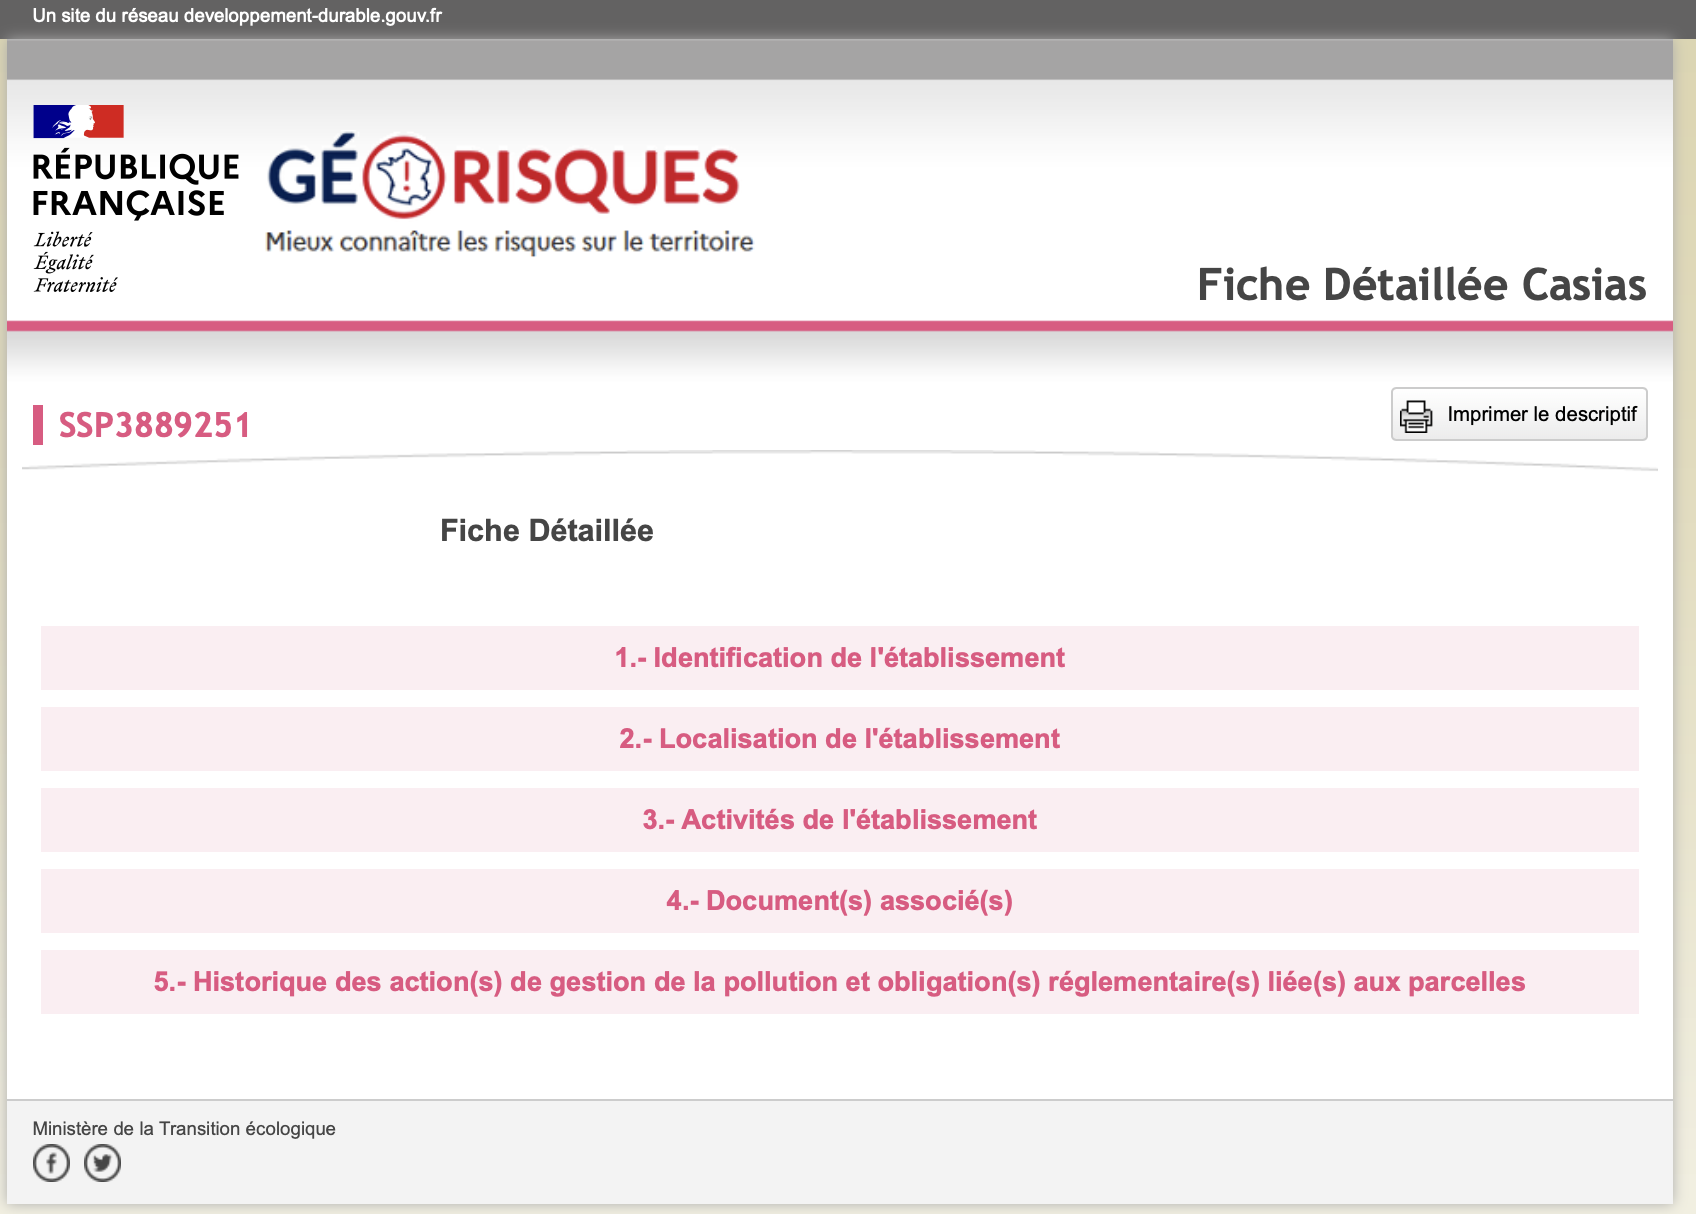
\includegraphics[width=0.75\textwidth]{img/chapitre3/Capture_Fiche_Riques_CASIAS}
\caption{Fiche risque CASIAS, site du ministère de l'Environnement}
\end{figure}

La fiche risque détaillée comporte des informations extrêmement utiles pour l'étude de la pollution des sols, notamment : 

\begin{itemize}
    \item les anciennes activités du site, codifiées avec la norme NAF 2008 (systématique)
    \item les dates d'exploitation du site (très inégal)
    \item  les propriétaires successifs (inégal)
    \item  la fiche administrative CASIAS (systématique)
\end{itemize}

\subsection{ActiviPoll v3 : corrélation entre activités et polluants}

\begin{quote}
« Il faut souligner que la base de données CASIAS est une cartographie de l’histoire des activités industrielles ou de services qui se sont succédées au cours du temps sur un territoire, et ne préjuge pas de la pollution effective des sols des établissements recensés. »\footnote{\cite{brgm_casias_nodate}}. 
\end{quote}
Si la cartographie des anciennes activités industrielles ne préjuge pas de la pollution effective des sols, elle permet \textbf{d’établir une suspicion de pollution et de la modéliser}. C’est dans cette optique que nous avons croisé nos données CASIAS avec la base de données \textbf{ActiviPoll v3} élaborée par le \textbf{service de géologie national} (BRGM). La base de données ActiviPoll \begin{quote}"répertorie et qualifie les corrélations entre les activités industrielles et les polluants qui peuvent leur être associés d'après le croisement de diverses sources d'information (bases de données françaises et littérature internationale spécialisée)"\footnote{\cite{brgm_bd_nodate}}\end{quote} Cette base de données recense les émissions de substances polluantes dans l'air, l'eau et les sols, ainsi que les installations à risque potentiel. 

« Etablissement public de référence dans les applications des sciences de la Terre pour gérer les ressources et les risques du sol et du sous-sol dans une perspective de développement durable », le BRGM a créé la base de données ActiviPoll en 2015\footnote{\cite{brgm_bd_nodate}}. C'est une base de donnée de production scientifique, commandée par le ministère de l'Environnement au BRGM dans le cadre de sa politique de gestion des sites pollués, tout juste renforcée par la loi ALUR en 2014\footnote{\cite{aubert_n_elaboration_2014}, page 3, la constitution de la base de donnée est l'action 10 programme annuel MEDDE-BRGM en 2014} . La base consiste en une \textbf{matrice de corrélation à double entrée croisant les activités humaines avec des substances et groupes de substances polluants potentiels émis pendant toute la durée de l'activité}. Nous utilisons la 3e version de cette base pour notre mémoire, mise à jour en 2018. 

% Capture notation ActiviPoll v3
\begin{figure}[!h]
\centering 
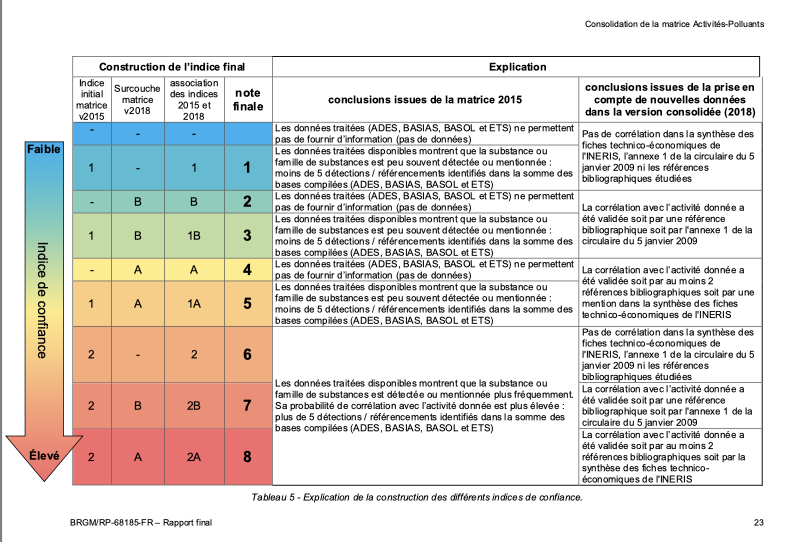
\includegraphics[width=0.75\textwidth]{img/chapitre3/BRGM_ActiviPol_Tableau}
\caption{BD ActiviPoll v3, schéma explicatif de la note finale d'hypothèse de pollution}
\end{figure}

La base de données ActviPoll est basée sur une \textbf{grille de notation allant de 0 à 8}. Plus cette note est élevée, plus la probabilité d'une contamination à une substance donnée est probable. La note de 8 correspond à l'indice maximal de confiance sur une contamination potentielle des sols, de l'eau ou de l'air. Les notes de 6 à 8 indiquent une corrélation très probable, les notes de 3 à 5 une corrélation plus hypothétique, et les notes de 1 à 2 une absence de corrélation. (voir figure 3.4)

\subsection{Le code NAF 2008 : indispensable pour croiser les données}

Afin de modéliser des hypothèses de pollution en Île-de-France, il fallait donc croiser la base de points CASIAS avec les corrélations ActiviPoll. Pour cela, nous avons récupéré les codes activités NAF 2008 associés à chaque ligne de la base. Commun à CASIAS et à la BD ActiviPoll v3, le code NAF 2008 est la clé indispensable pour croiser les deux bases de données. Le code NAF 2008, ou Nomenclature d'Activités Française, est le système de classification des activités économiques de référence en France, dont la dernière révision date de 2008. Élaboré par l'INSEE, il vise à identifier de manière précise et homogène les secteurs d'activité des entreprises et de leurs établissements. Chaque code NAF est constitué de quatre chiffres suivis d'une lettre, formant un identifiant unique pour les différentes branches d'activité. Cette nomenclature est essentielle pour les analyses statistiques économiques, la réglementation administrative et les politiques publiques, permettant une meilleure compréhension et gestion des dynamiques économiques nationales. Elle est utilisée dans CASIAS pour affilier à chaque site un type d'activités, et dans ActiviPoll pour associer à chaque code une probabilité de pollution. 

% Capture fiche risque web 2 (zoom)
\begin{figure}[!h]
\centering 
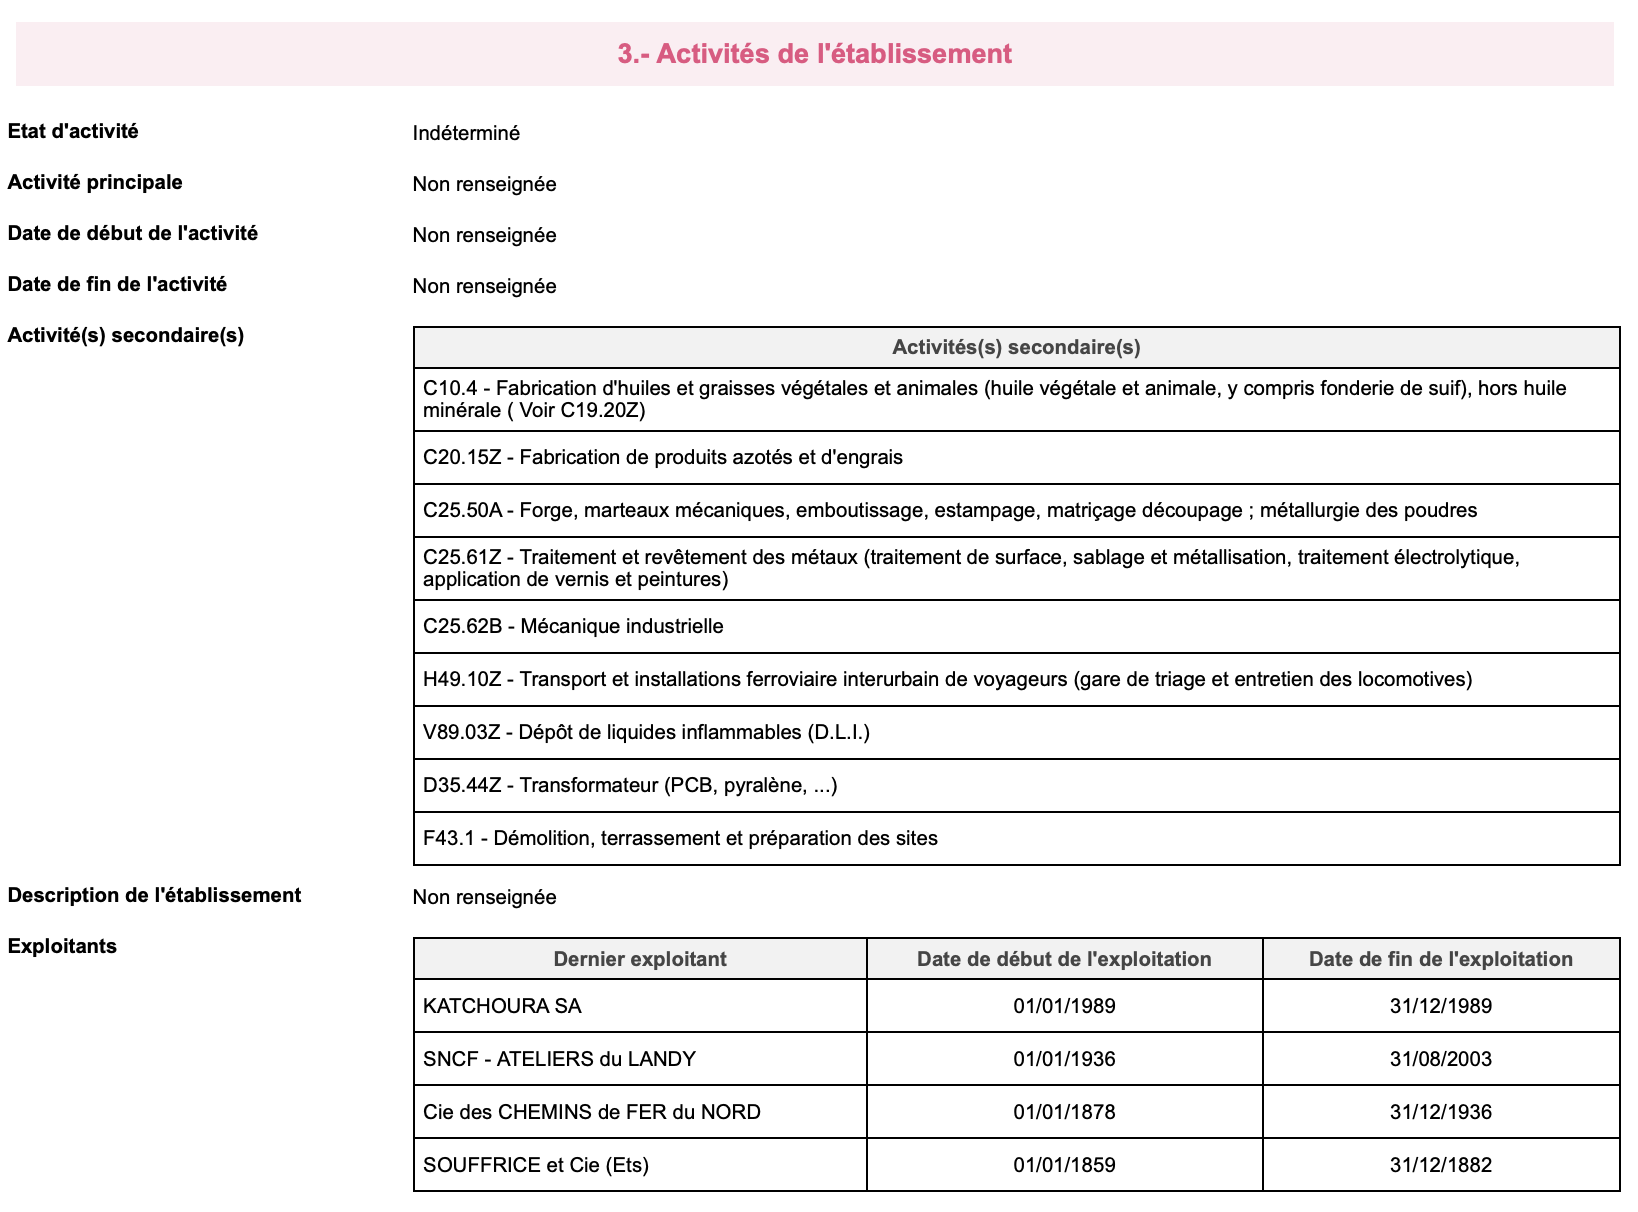
\includegraphics[width=0.8\textwidth]{img/chapitre3/CASIAS_FICHE_RISQUE_ZOOM_NAF2008}
\caption{Fiche risque CASIAS, exemple de codes activités attachés à un site}
\end{figure}
        
\subsection{Notre chaîne de traitement}

Pour exploiter nos deux bases de données source, nous avons fait le choix de construire une chaîne de traitement combinant des scripts en Python et en R (voir figure \ref{fig:pipeline}). Les scripts python nous ont servi à réaliser toutes les tâches de moissonnage et de préparation des données source, ainsi que nos cartes dynamiques (consultables sur notre dépôt GitHub). Les scripts R nous ont ensuite servi à réaliser les étapes d’analyse spatiale, de modélisation, et de cartographie statique. 

% Schéma pipeline Python 
\begin{figure}[!h]
\centering 
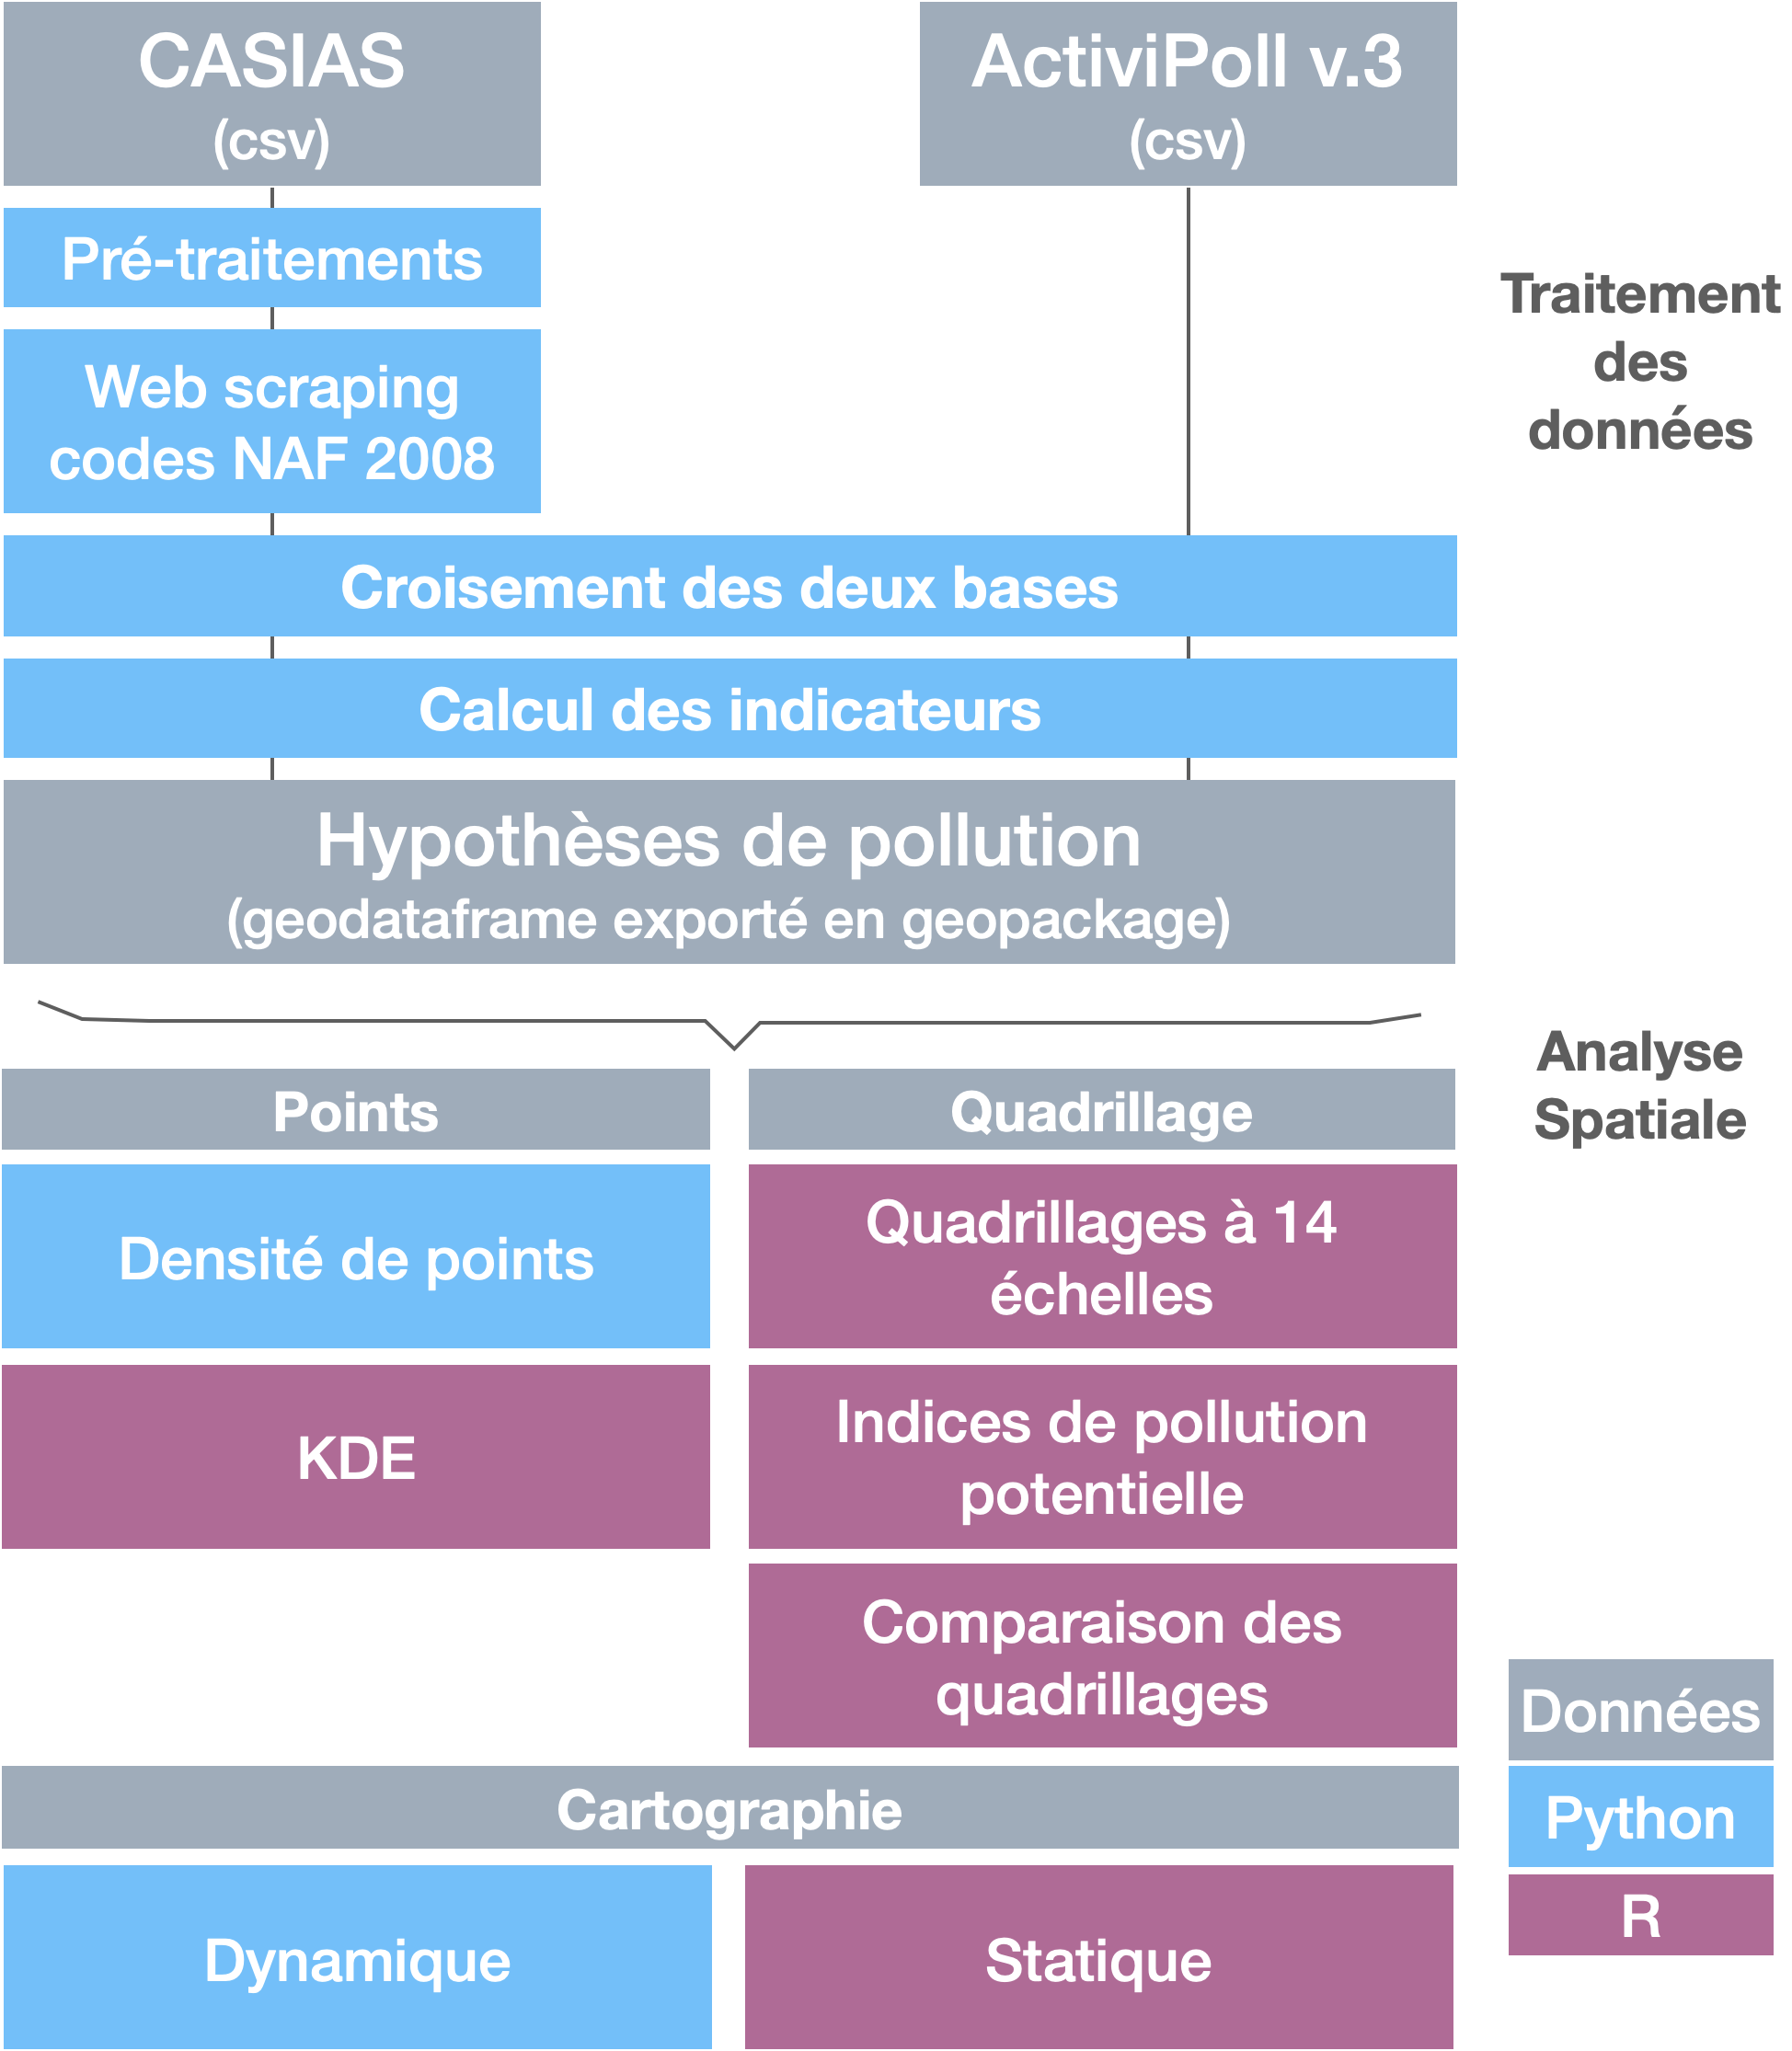
\includegraphics[width=0.75\textwidth]{img/chapitre3/schema_pipeline_all.png}
\caption{Schéma de notre chaîne de traitement complète}
\label{fig:pipeline}
\end{figure}

Nous avons extrait les données brutes CASIAS pour la région Île-de-France au format csv (voir l'extrait de tableau en figure \ref{fig:casias_donnees_brutes}), directement sur la page dédiée de la plateforme Géorisques. Chaque site répertorié dans la base de données CASIAS possède un identifiant Sites et Sols Pollués (SSP) unique et une fiche risque, tous deux listés dans le tableau extrait. Cette fiche risque recense les informations administratives règlementaires pour la gestion du risque industriel, et recoupe les informations recueillies lors des campagnes d’archives. Pour chacune des 36 739 lignes CASIAS, nous avons pris l’adresse url de ces fiches risque. Grâce à ces url, nous avons récupéré en ligne les fiches risques en format HTML, découpé\footnote{"parsé"} ces fichiers HTML et extrait les codes NAF 2008 associés aux activités des lieux. Ces codes NAF 2008 nous ont ensuite permis de récupérer la note de probabilité de pollution associée à chacun des soixante-douze sous-groupes de substances listés dans ActiviPoll. Chaque site pouvant lister plusieurs activités, un sous-groupe de polluants peut être corrélé plusieurs fois au même site. Dans ce cas, la note de corrélation la plus haute est attribuée au sous-groupe en doublon sur le site. En théorie, la base de données ActiviPoll liste des milliers de substances polluantes connues. Le BRGM recommande toutefois de ne pas descendre au niveau des substances individualisées, pour des raison de solidité statistique (intervalles de confiance trop faibles). Nous avons suivi ces recommandations, en effectuant nos analyses à l'échelle des groupes et sous-groupes de substances. 

Quoique le niveau de détail de la base de données ActiviPoll soit extrêmement intéressant pour entrer dans le détail des sites, il tend à offrir une vue fragmentée de la pollution. Si cette approche est la plus scientifiquement viable du point de vue des sciences naturelles, de l'étude de la pollution en tant que phénomène physique, elle limite la montée en généralité d'une analyse de la pollution d'un point de vue de sciences sociales. Nous n'excluons pas complètement une analyse par sous-groupes, les PFAS dont nous avons déjà beaucoup parlé sont un sous-groupe dans la base ActiviPoll. Mais nous avons cependant cherché à monter en généralité dans la modélisation de la pollution des sols, pour la saisir comme un phénomène spatial d'ensemble. La mobilisation des sous-groupes s'avèrera sans doute très utile pour l'analyse de la pollution selon les secteurs d'activités industrielles, travail que nous n'avons pas pu inclure dans ce mémoire mais que nous prévoyons pour la suite. Nous avons donc calculé la note moyenne de pollution pour les six grands groupes de substances listés dans CASIAS, chaque sous-groupe s'attachant à l'un de ces six grands groupes (voir figure \ref{fig:schema_Activi_Poll}). Pour chaque groupe de substances, nous prenons la moyenne arithmétique des notes de pollution des sous-groupes qui la composent. Il est ainsi possible d'effectuer aisément des analyses par groupes de substances et sous-groupes de substances. Publié après le début de nos travaux, l'article \og{} Développement d'un indice spatialisé de pollution potentielle en éléments traces métalliques des sols urbains en Île-de-France\fg{}\footnote{Article publié en 2024 dans \cite{charvet_sols_2024} par Mathilde Basuyau, Laure Chabalier et Philippe Branchu}, corrobore cette méthodologie : la moyenne arithmétique des métaux et métalloïdes (ou éléments traces métalliques) servant de base à leur analyse.  

Enfin, nous mettons deux autres indicateurs agrégés au banc d'essai de notre étude : la note moyenne de pollution, et la somme des substances présentes. Nous calculons la note moyenne de pollution par une simple moyenne arithmétique de toutes les notes de pollution des sous-groupes d'un site (sur le même modèle que la note moyenne des six groupes). Nous souhaitions par là aller plus loin dans la généralisation, en produisant un indicateur unique pour synthétiser toutes les hypothèses de pollution sans sous-diviser l'étude par groupes de substances. Cette moyenne de moyenne cumulant doublement toutes les limites connues de cet outil statistique, cet indicateur est ensuite manipulé avec toutes les précautions d'usage. Nous souhaitions cependant comparer son comportement avec les autres hypothèses de pollution modélisées. Notre dernier indicateur cherche à modéliser le cocktail toxique potentiel présent en un point. Des études en toxicologie ont mis en évidence que les interactions entre polluants peuvent avoir des effets significatifs sur la toxicité globale présente dans les écosystèmes\footnote{Koelmans et al. (2009), "Combined effects of toxicants on ecological systems: synergistic and antagonistic interactions"}. Nous sommons donc les substances co-présentes dans le sol en un point, afin de quantifier ce phénomène de sur-toxicité. 

Une ultime étape de nettoyage ôte les dernières scories (voir sous-partie 3.2.1). Nos hypothèses de pollution finales sont stockées dans un nouveau dataframe, une copie enrichie du dataframe CASIAS d'origine. Nous vérifions le système de projection des données, et nous les transformons en objet géographique (geodataframe). Nous sauvegardons deux projections des données dans un geopackage, l'une en système projeté français Lambert93 pour nos analyses spatiales, l'autre en système géodésique international WGS84 pour les cartes dynamiques.  

%Nous avons enfin agrégé spatialement ces données, à l'échelle du point CASIAS géolocalisé. 

La datation des sites CASIAS dans les fiches risques des sites n'est pas systématique, et est de qualité hétérogène. Une minorité de sites liste précisément les dates d'ouverture et de fermeture des sites, gardant même une trace des différentes entreprises ayant opéré sur les lieux. Il s'agit le plus souvent des sites industriels les plus notables, ou de sites publiques. L'ancienne usine à gaz du Cornillon exploitée par Gaz de France jusqu'en 1963 en est un bon exemple. Toutefois, la qualité des données de datation étant trop médiocre pour être significative, nous avons fait le choix de ne pas inclure les dates d'exploitation des sites dans notre moissonnage de données. Nous avons donc renoncé à construire une analyse diachronique du système spatial industriel pour ce mémoire, au-delà de ses grands mouvements de ruptures synthétisé dans le premier chapitre sur la base de travaux historiens. Nous espérons pouvoir poursuivre nos travaux et développer cette analyse diachronique après le rendu de notre mémoire. Cette contrainte technique nous force à adopter un positionnement chronologique qui demeure intéressant. Notre focale sur le passé est ancré en 2024, et nous permet d'analyser la pollution du point de vue de son accumulation dans l'environnement. Nous sommes obligés d'adopter un regard qui embrasse notre héritage industriel toxique dans toutes ses strates temporelles. Les données CASIAS les plus anciennes datent du début du \siecle{XIX}, correspondant à peu près à l'accélération de l'industrialisation en France. Malgré cette borne temporelle imprécise, ces données nous offrent la possibilité d'ébaucher   une analyse du système spatio-temporel \footnote{\cite{grataloup_christian_introduction_2023}, page 86} contemporain de la pollution des sols. 

% Dessin 6 groupes et 72 sous-groupes
\clearpage
\begin{figure}[!h]
	\begin{minipage}[c]{.5\linewidth}
        		\begin{center}
        			 \begin{tikzpicture}[scale=0.5, transform shape] %Chimique 
           			 \tikzstyle{maincircle} = [circle, draw, minimum size=2cm, text centered, align=center, fill=blue!20]
            			\tikzstyle{smallcircle} = [circle, draw, minimum size=1cm, text centered, align=center, fill=white]
            			\node[maincircle] (A) {Chimique};
            			\node[smallcircle, above left=1cm and 1cm of A] (A1) {Param. azotés};
            			\node[smallcircle, above=1cm of A] (A2) {Param. phosphorés};
            			\node[smallcircle, above right=1cm and 1cm of A] (A3) {Radioactifs};
            			\foreach \i in {1,2,3}
            			{
				\draw (A) -- (A\i);
				}
        			\end{tikzpicture}
        		\end{center}
	\end{minipage}
	\begin{minipage}[c]{.5\linewidth}
        		\begin{center}
		\begin{tikzpicture}[scale=0.5, transform shape] %Elements minéraux
           		\tikzstyle{maincircle} = [circle, draw, minimum size=2cm, text centered, align=center,fill=red!20]
            		\tikzstyle{smallcircle} = [circle, draw, minimum size=1cm, text centered, align=center, fill=white]
            		\node[maincircle] (B) at (0,0) {Eléments minéraux};
            		\node[smallcircle, above left=1cm and 1cm of B] (B1) {Amiante};
            		\node[smallcircle, above=1cm of B] (B2) {Composés chlorés};
            		\node[smallcircle, above right=1cm and 1cm of B] (B3) {Composés cyanurés};
            		\node[smallcircle, below left=0.5cm and 1cm of B] (B4) {Composés soufrés};
            		\node[smallcircle, below right=1cm and 1cm of B] (B5) {Autres};
            		\foreach \i in {1,2,3,4,5}
            		{
                		\draw (B) -- (B\i);
            		}
        		\end{tikzpicture}
		\end{center}
	\end{minipage}
\end{figure}

\begin{figure}[!h]
	\begin{minipage}[c]{.5\linewidth}
        		\begin{center}
		 \begin{tikzpicture}[scale=0.5, transform shape] %Métaux
    			\tikzstyle{maincircle} = [circle, draw, minimum size=2cm, text centered, align=center, fill=lime!30]
    			\tikzstyle{smallcircle} = [circle, draw, minimum size=1cm, text centered, align=center, fill=white]
    			\node[maincircle] (C) at (0,0) {Métaux et métalloïdes};
    			\foreach \name/\angle in {Aluminium/24, Arsenic/48, Cadmium/72, Chrome/96, Cuivre/120, Fer/144, Magnésium/168, Manganèse/192, Mercure/216, Molybdène/240, Nickel/264, Plomb/288, Uranium/312, Zinc/336, Autres/360}
   			{
       			\node[smallcircle] (\name) at (\angle:4cm) {\name};
        			\draw (C) -- (\name);
    			}
		\end{tikzpicture}
        		\end{center}
	\end{minipage}
	\begin{minipage}[c]{.5\linewidth}
        		\begin{center}
		\begin{tikzpicture}[scale=0.5, transform shape] %Pharmaceutiques
   			\tikzstyle{maincircle} = [circle, draw, minimum size=2cm, text centered, align=center, fill=orange!20]
    			\tikzstyle{smallcircle} = [circle, draw, minimum size=1cm, text centered, align=center, fill=white]
    			\node[maincircle] (D) at (0,0) {Pharmaceutiques et hormones};
    			\foreach \name/\angle in {Anti-inflammatoires/40, Antibiotiques/80, Stéroïdes et hormones/120, Anti-cancéreux/160, Anti-épileptique/200, Bétabloquants/240, Hypolipidémiants/280, Psychotropes/320, Autres/360}
    			{
        			\node[smallcircle] (\name) at (\angle:5cm) {\name};
        			\draw (D) -- (\name);
    			}
		\end{tikzpicture}
		\end{center}
	\end{minipage}
\end{figure}


\begin{figure}[!h]
	\begin{minipage}[c]{.4\linewidth}
        		\begin{center}
		 \begin{tikzpicture}[scale=0.5, transform shape]
    		\tikzstyle{maincircle} = [circle, draw, minimum size=2cm, text centered, align=center, fill=yellow!20]
    		\tikzstyle{smallcircle} = [circle, draw, minimum size=1cm, text centered, align=center, fill=white]
    		\node[maincircle] (D) at (0,0) {Phytosanitaires};
		\foreach \name/\angle in {Acaricides/45, Fongicides/90, Herbicides/135, Insecticides/180, Nématicides/225, Régulateurs de croissance/270, Rodenticides/315, Autres/360}
    		{
        		\node[smallcircle] (\name) at (\angle:5cm) {\name};
       		\draw (D) -- (\name);
    		}
		\end{tikzpicture}
        		\end{center}
	\end{minipage}
	\begin{minipage}[c]{.6\linewidth} %(x,y)
        		\begin{center}
		\begin{tikzpicture}[scale=0.5, transform shape]
		\begin{scope}[every node/.style={circle, draw}]
			\node[fill=cyan!20] (A) at (0,0) {Micropolluants organiques};
			\node (B) at (3.75,-1.5) {Chloroalcanes};
			\node (D) at (2.75,1.5) {SCCP};
			\node (O) at (2,-2.75){COHV};
			\node (N) at (2,2.75){Fréons};
			\node (P) at (0.5,3.1){BTEX};
			\node (U) at (-0.75,3){HAP};
			\node (Y) at (-2,2.5){PFC};
			\node (V) at (-3,1.5){Nitriles};
			\node (AB) at (-3,0){PCB};
			\node (AF) at (-3.4,-1.5){Phtalates};
			\node (C) at (-3.2,-3.3) {Amines};
			\node (S) at (-1.5,-3){Autres};
			\node (AC) at (0.3,-4.2){Chlorophénols};
			
			\node (X) at (4.2,2.5){\shortstack{PBDE et \\ PBB}};
			\node (F) at (5.1,0.6){\shortstack{Additifs \\d'essence}};
			\node (H) at (-4.7,-4.7){\shortstack{Alcools et \\polyols}};
			\node (E) at (-5.2,0.1){\shortstack{Acides \\carboxyliques}};
			\node (AI) at (3.7,-7.4){\shortstack{Urée et \\métabolites}};
			\node (AE) at (3.25,-4.7){Chlorobenzènes};
			\node (I) at (-2.6, 4.3){\shortstack{Aldéhydes et \\cétones}};
			\node (J) at (0,5.1){Alkylphénols};
			\node (Q) at (7.3,0.9){\shortstack{Dérivés du \\Benzène}};
			\node (R) at (-5.3,-2.5){Carbamates};
			\node (L) at (8.2,-3.4){\shortstack{Anilines et \\dérivés}};
			\node (M) at (5.2,5){\shortstack{Solvants \\ chlorés}};

			\node (G) at (-4.7,2.7){\shortstack{Additifs du \\1,1,1 TCA}};
			\node (K) at (0.9,-7.2){\shortstack{Nonylphénols et\\ bisphénols A}};
			\node (W) at (6.4,3.1){\shortstack{Organo-\\phosphorés}};
			\node (Z) at (2.75,4.75){Hydrocarbures};
			\node (AA) at (5.9,-6.4){\shortstack{Dioxines et \\Furanes}};
			\node (AD) at (6.5,-1.5){\shortstack{Phénol crésol \\et dérivés}};
			\node (AG) at (5.9,-4){\shortstack{Triazines et \\métabolites}};
			\node (AH) at (-2.2,-5.8){Trihalométhanes};
			
			
		\end{scope}
	
		\begin{scope}
			\draw (A)--(B);
			\draw (A)--(C);
			\draw (A)--(D);
			%\draw (A)--(E);
			\draw (A)--(F);
			%\draw (A)--(G);
			%\draw (A)--(H);
			%\draw (A)--(I);
			%\draw (A)--(J);
			%\draw (A)--(K);
			%\draw (A)--(L);
			%\%draw (A)--(M);
			\draw (A)--(N);
			\draw (A)--(O);
			\draw (A)--(P);
			%\draw (A)--(Q);
			%\draw (A)--(R);
			\draw (A)--(U);
			\draw (A)--(V);
			%\draw (A)--(W);
			%\draw (A)--(X);
			\draw (A)--(Y);
			%\draw (A)--(Z);
			%\draw (A)--(AA);
			\draw (A)--(AB);
			\draw (A)--(AC);
			%\draw (A)--(AD);
			%\draw (A)--(AE);
			\draw (A)--(AF);
			%\draw (A)--(AG);	
			%\draw (A)--(AH);
			%\draw (A)--(AI);
			\draw (A)--(S);
		\end{scope}
		\end{tikzpicture}
		\end{center}
	\end{minipage}

\caption{Groupes et sous-groupes de substances pris en compte dans ActiviPoll v3}
\label{fig:schema_Activi_Poll}
\end{figure}

\section{Transformer les points CASIAS en lieux d'histoire}

\subsection{Nettoyage des données}

La base de données CASIAS nous fournit des données massives sur l'industrialisation de l'Île-de-France avec 36 738 points extraits dans toute la région. Avant de procéder à la première cartographie de ces points, nous avons dû nettoyer la base et mettre en qualité les données. Nous avons vérifié le type de données des variables, et rectifié le code postal en integer64\footnote{Int64 décrit un nombre entier. Float64 décrit un nombre décimal}, unifié le nom des établissements en supprimant les accents et ponctuations, et remplacé les valeurs nulles par zéro en prévision pour la suite de nos traitements. La figure \ref{fig:cleancasias} synthétise le type des variables et leur nombre avant et après le nettoyage des données. On remarque ainsi que si tous les sites font l'objet d'une fiche, permettant au moins de leur rattacher une commune, seuls 62\% des sites recensés ont un nom d'établissement (22 937), et 13\% des sites ne sont pas géoréférencés. Après suppression des 4 866 sites concernés, nous obtenons notre base de travail finale, comptant 31 872 points CASIAS croisés avec succès avec la base de données ActviPoll v3. 

% Table de nettoyage des variables
\begin{table}[h]
\centering
\small
\caption{Exploration CASIAS}
\label{fig:cleancasias}
\begin{tabular}{>{\raggedright\arraybackslash}p{3.5cm} >{\raggedright\arraybackslash}p{3cm} >{\raggedright\arraybackslash}p{2.5cm} >{\raggedright\arraybackslash}p{3cm} >{\raggedright\arraybackslash}p{2.5cm}}
    \toprule
    Variable & Data type avant & Compte avant & Data type après & Compte après \\
    \midrule
    code\_metier & object & 36 738 & object & 31 872 \\
    nom\_inventaire & object & 36 738 & object & 31 872 \\
    code\_inventaire & object & 36 738 & object & 31 872 \\
    nom\_etablissement & object & 22 937 & object & 31 872 \\
    adresse & object & 36 738 & object & 31 872 \\
    code\_postal & float64 & 35 199 & int64 & 31 872 \\
    code\_insee & int64 & 36 738 & int64 & 31 872 \\
    nom\_commune & object & 36 738 & object & 31 872 \\
    code\_departement & int64 & 36 738 & int64 & 31 872 \\
    nom\_department & object & 36 738 & object & 31 872 \\
    code\_region & int64 & 36 738 & int64 & 31 872 \\
    nom\_region & object & 36 738 & object & 31 872 \\
    etat\_activite & object & 36 738 & object & 31 872 \\
    nature\_localisation & object & 36 738 & object & 31 872 \\
    x\_wgs84 & float64 & 31 879 & float64 & 31 872 \\
    y\_wgs84 & float64 & 31 879 & float64 & 31 872 \\
    fiche\_risque & object & 36 738 & object & 31 872 \\
    \bottomrule
\end{tabular}
\end{table}

\subsection{Comprendre la géolocalisation des sites}

% Encadré carte dynamique des duplicats 
\begin{tcolorbox}[colback=gray!5!white,colframe=gray!20!white]
La carte dynamique \textbf{des points duplicats} est disponible sur notre dépôt Git Hub : \url{https://charlotte-berthier.github.io/heritages_toxiques/cartes_dynamiques/carte_duplicate_points.html}.
\end{tcolorbox}

Une dernière chose restait à faire pour prendre en main notre jeu de données : comprendre la stratégie de géolocalisation des sites. En regardant de plus près les sites non géoréférencés supprimés, nous comprenons que la localisation des sites résulte du géocodage des adresses historiques recensées lors des campagnes d’archives. En l'absence de documentation sur la procédure appliquée par l'administration, nous supposons l'emploi de la stratégie la plus simple par l'administration : l'utilisation d'un géocodeur en langage python ou R sur les adresses historiques, par exemple Nominatim de l'univers Open Street Map. 

Le plus souvent, ces adresses n'ont pas été géocodées en raison d'erreurs dans l'adresse mentionnée en base (parenthèses mal placées, ordre des mots erroné, orthographes aberrantes, etc.). D'autres cas pourraient correspondre à des adresses n'existant plus dans le système postal contemporain, qui nécessiteraient donc l'emploi de géocodeurs historiques. La variable \og{} nature\_localisation \fg{} de CASIAS nous révèle que 10\% des adresses géocodées ont été vérifiées manuellement par l'administrateur. Il semble donc logique que des erreurs se soient glissées dans les 90\% restants. Réparties sur tous le territoire francilien, ces erreurs ne nous semblaient pas significativement impacter la représentativité de la base CASIAS, d'où notre décision de les en supprimer. Les erreurs de géocodage étant principalement liés à des adresses erronées, nous avons investigué des méthodes de reconnaissance d'entités nommées (NER) pour récupérer les adresses erronées. L'objectif était et lancer un nouveau géocodage en découpant les adresses et en les remettant dans l'ordre . Cette tâche nous a rapidement posé beaucoup de difficultés, du fait de l'hétérogénéité d'encodage des adresses. Le rapport bénéfice / temps de développement dans les délais impartis pour produire notre mémoire nous a fait trancher en défaveur de la poursuite de cette tâche. 

Enfin nous avons examiné les points en doublon dans la base de données CASIAS, que nous nommerons duplicats. Deux duplicats sont des points possédant exactement les mêmes coordonnées xy. Ils sont donc exactement superposés sur la carte. En examinant nos données, 497 couples de coordonnées sont concernés, avec une moyenne de 2.15 sites par point dupliqué. Afin de mieux visualiser ces points et de les analyser, nous avons codé une carte dynamique laissant apparaître les métadonnées de chaque point. En analysant la répartition des duplicats, nous cherchions à comprendre : 

\begin{itemize}[label ={\textbf{\textbullet}}]
\item si ces doublons étaient des points \og{} décharges \fg{} par commune, un point rassemblant les sites mal géocodés\footnote{Nous avions entendu parler de cette stratégie de géocodage de données historiques lors du séminaire de l'ANR SODUCO en novembre 2023} 
\item la raison de l'existence de ces doublons
\item s'il fallait conserver ces doublons dans la base pour la suite de notre étude 
\end{itemize}

% Carte des duplicats zoom Paris
\begin{figure}[!h]
\centering 
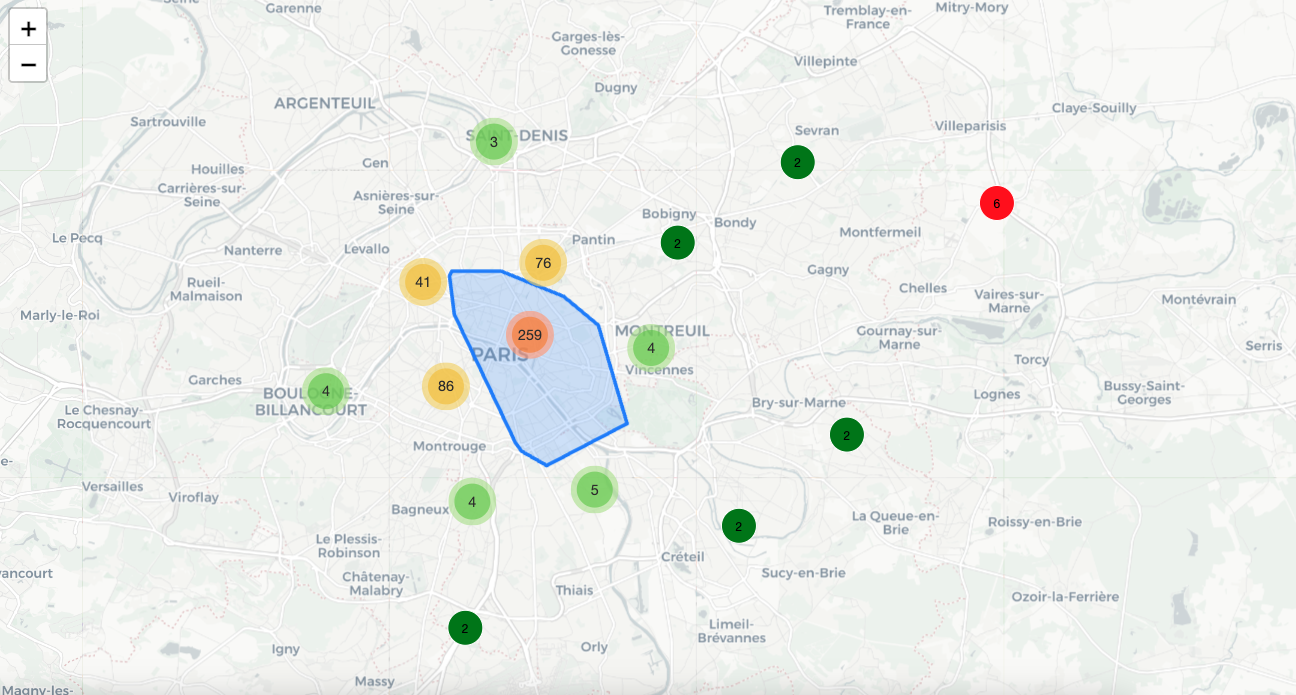
\includegraphics[width=0.75\textwidth]{img/chapitre3/CASIAS_Carte_duplicats_ZoomParis.png}
\caption{Carte dynamique des points duplicats - extrait}
\label{fig:duplicatszoomparis}
\end{figure}

Nous avons confirmé que l'administration n'a pas eu recours à une stratégie de points décharges par commune. Nous ne trouvons aucune preuve de point unique rassemblant tous les sites mal référencés (qui aurait pu se trouver autour du centroïde de la commune). Nous établissons trois causes principales expliquant la présence de points duplicats, la premières certaine et vérifiable dans les données, les deux autres hypothétiques mais vérifiables par un retour à la lecture proche des archives de chaque site :

\begin{itemize}[label ={\textbf{\textbullet}}]
	\item Les \textbf{erreurs de géocodage} 
	\begin{itemize}[label={\color{black}$\circ$}]
		\item Numéros de rue
		\item Ancien système d'adresses
		\item Adresses contemporaines aberrantes
	\end{itemize}
	\item La \textbf{co-présence d'activités} sur un même site
	\item La \textbf{succession d'activités} sur un même site 
\end{itemize}

La carte dynamique par clusters des duplicats révèle que la majorité de ceux-ci se trouvent dans Paris intra-muros, particulièrement dans les anciens quartiers et faubourgs ouvriers de l'est depuis les Halles jusqu'au XIIIe, XIIe et XXe arrondissements (cf. figure \ref{fig:duplicatszoomparis}). Cela est proportionnellement en cohérence avec la plus grande concentration de points CASIAS dans Paris intra-muros (voir figure \ref{fig:nb_sites_dept_bleu}). Cela conforte également notre connaissance préalable du système de production à Paris au tournant du \siecle{XIX} (cf. chapitre 1). Les duplicats observés dans Paris ne sont pas le fruit d'erreurs de géocodage. La succession du même type d'activités dans un même local\footnote{L'étude des annuaires de commerce de Paris au \siecle{XIX} dans le cadre de l'ANR SODUCO a permis de tracer l'évolution du tissu économique parisien, notamment de suivre les changements de propriétaires d'un même local dans le temps.} comme la co-présence\footnote{Voir \cite{gribaudi_ruptures_2009} sur le foncier de la Trinité dans le quartier des Halles et le développement des petits ateliers)} de plusieurs activités dans un même immeuble sont typiques de l'artisanat et de la proto-industrialisation présentes à Paris aux XVIIIe et \siecle{XIX} siècles. Ainsi, nous pensons que les points duplicats dans Paris centre ne sont pas des erreurs, mais des traces de l'organisation spatiale des activités de production qui a précédé celle de l'industrialisation de l'Île-de-France. 

En revanche, les duplicats observés en petite et grand couronne sont majoritairement le produit d'erreurs de géocodage, que ce soit par erreur sur les numéros de rue ou par géocodage aberrant. Les extraits de carte en figure \ref{fig:duplicats_erreurs_geocodage} montrent respectivement un point duplicat confondant Montrouge et Asnières, et le regroupement de plusieurs numéros de rue en un même point. Quelques cas correspondent aux mêmes hypothèses de co-présence ou de succession d'établissement qu'à Paris, mais ils sont rares. La différence de nature des duplicats entre Paris et le reste de l'Île-de-France renforce notre hypothèse selon laquelle les points intra-muros traduisent une réalité historique antérieure à l'industrialisation des banlieues.  

% Deux erreurs de géocodage
\begin{figure}[!h]
\centering
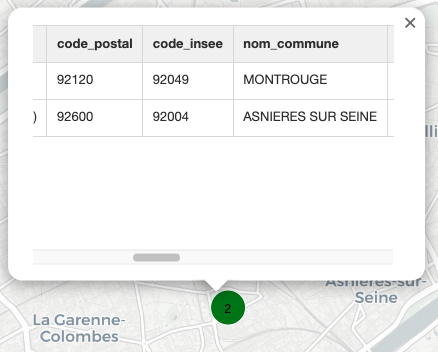
\includegraphics[width=0.4\textwidth]{img/chapitre3/Duplicats_errur_geocodage_Communes.png}
\includegraphics[width=0.4\textwidth]{img/chapitre3/Duplicats_Erreur_Numéro_Rue.png}
\caption{Duplicats - Deux exemples d'erreurs de géocodage}
\label{fig:duplicats_erreurs_geocodage}
\end{figure}

Nous avons donc décidé de supprimer les duplicats les plus aberrants, à savoir les points dupliqués ne se trouvant pas dans la même commune (cf. figure \ref{fig:duplicats_erreurs_geocodage}). Nous avons jugé sur les autres erreurs de géocodage, majoritairement des erreurs de numéros de rue, n'impacteraient pas significativement les résultats des modélisations ultérieures. Les autres points duplicats correspondent à des réalités historiques et spatiales dont il faut tenir compte dans l'analyse de la base de données. 

% Carte des points CASIAS avec les 2 points centraux - landscape
\begin{landscape}
\begin{figure}[htbp]
\centering 
\hspace*{-2cm}\vspace*{+2cm}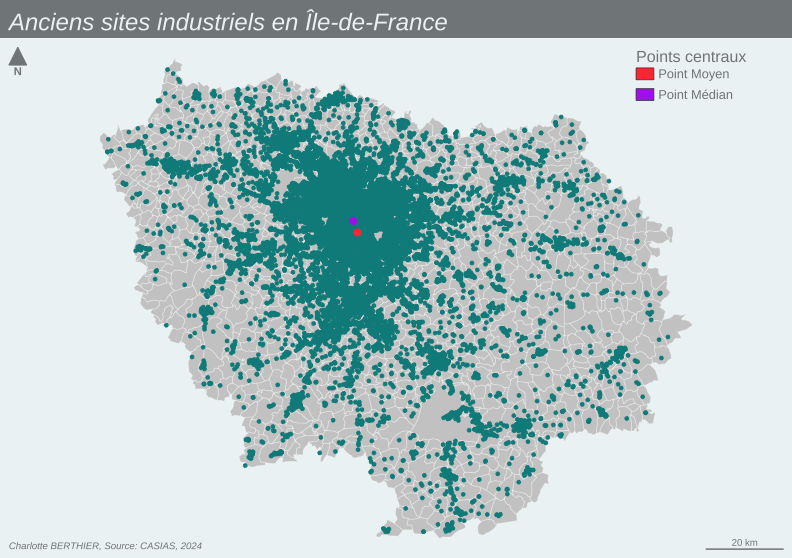
\includegraphics[width=1.35\textwidth]{img/chapitre3/CASIAS_Carte_IDF_All_Points_fixe_Moyen_Median.png}
\caption{Implantation des sites CASIAS en Île-de-France, localisation des points centraux}
\label{fig:carte_points_casias_bleue_points_centraux}
\end{figure}
\end{landscape}


%%%  3e sous-partie, les lieux d'histoire 
\section{Les lieux d'histoire de la pollution industrielle en Île-de-France}

% Encadré raccourci carte dynamique
\begin{tcolorbox}[colback=gray!5!white,colframe=gray!20!white]
La carte dynamique de la \textbf{répartition des sites CASIAS en Île-de-France} est disponible sur notre dépôt GitHub : \url{https://github.com/charlotte-berthier/heritages_toxiques/cartes_dynamiques/carte_points_ile_de_france.html}.
\end{tcolorbox}

La carte de répartition des sites CASIAS nous permet d'obtenir une première visualisation des lieux de l'industrialisation en Île-de-France. L'illisibilité de la carte statique \ref{fig:carte_points_casias_bleue_points_centraux} témoigne de la non homogénéité de la répartition des anciens sites industriels sur le territoire francilien. Afin d'explorer la répartition spatiale de nos points, nous avons donc codé une carte dynamique en python. Le recours aux clusters dynamiques avait pour objectif technique d'alléger le calcul des niveaux zooms. Ces clusters produisent \textit{de facto} une carte de chaleur qui confirme notre analyse visuelle : la densité de sites CASIAS va décroissante depuis le centre de Paris vers les confins de l'ïle-de-France, selon un gradient restant à définir, et selon une logique relativement concentrique. 

% Capture carte dynamique des points CASIAS
 \begin{figure}[!h]
\centering 
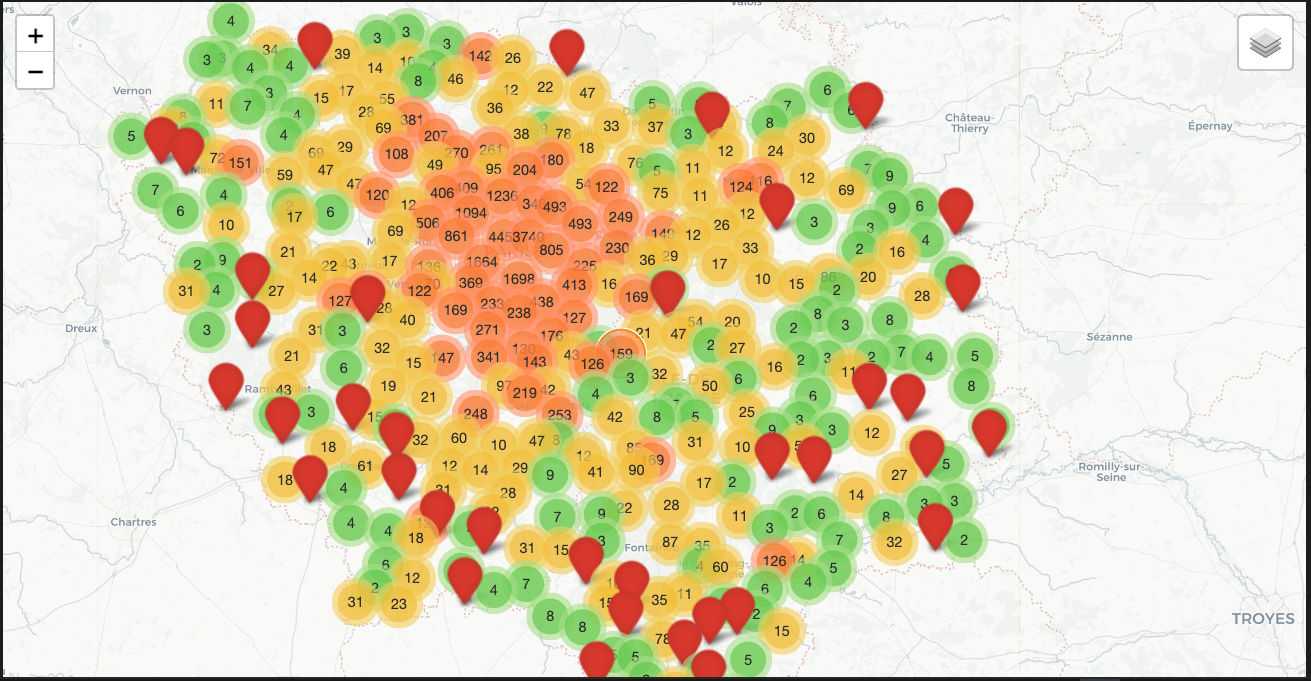
\includegraphics[width=0.75\textwidth]{img/chapitre3/CASIAS_Carte_Points_Folium.png}
\caption{Extrait de la carte dynamique des points CASIAS}
\label{fig:carte_cluster_casias}
\end{figure}

Cette première visualisation du système spatial de l'industrialisation en Île-de-France semble corrélée à l'extension urbaine francilienne\footnote{\cite{gallet_atlas_2020}}. La densité de sites industriels semble donc diminuer avec le taux d'urbanisation, et suivre la très classique loi d'agglomération de Clark\footnote{En économie urbaine}, stipulant que les activités économiques ont tendance à se regrouper dans les zones les plus denses. Cette hypothèse se vérifie quantitativement par le calcul des points centraux et des distances type du semis de points. Nous avons effectué l'analyse spatiale du semis de points en Python, à la fin de l'exploration des données CASIAS (cf. figure \ref{fig:pipeline}). 

Les points centraux du système spatial industriel se situent au centre de Paris, légèrement à l'Est. Le centre de gravité du semis de point, c'est-à-dire le point moyen pondéré, confirme le poids de Paris et de la petite couronne dans le système industriel francilien. Le point moyen, en rouge sur la carte \ref{fig:carte_points_casias_bleue_points_centraux}, se situe dans le XIIIe arrondissement, dans le campus hospitalier de la Salpétrière. Son positionnement rive gauche et légèrement à l'Est est cohérent avec les dimensions de la région Île-de-France, plus étendue vers le Sud. Le point médian, plus représentatif de la répartition des points, se trouve lui dans le IIIe arrondissement, 60 rue Chapon en plein quartier des Halles. Le centrage de ces deux points correspond à ce que nous connaissons de l'histoire industrielle de Paris, qui favorisa l'implantation des sites nauséabonds à l'Est, sous le vent. Le positionnement du point médian en plein quartier des Halles souligne l'intensité industrielle historique du ventre de Paris, et l'intensité de l'industrialisation des banlieues Nord et Est. 

\begin{tcolorbox}[colback=gray!5!white,colframe=gray!20!white]

\textbf{Le point moyen}
"Le point moyen non pondéré est le point G dont les coordonnées sont égales à la moyenne des coordonnées en X (mX) et la moyenne des coordonnées en Y (mY). Il définit le centre de gravité du nuage de points."\footnote{Source : \url{http://grasland.script.univ-paris-diderot.fr/go303/ch1/ch1.htm}} 

\textbf{Le point médian}
"Soit un ensemble de points 1..i..N distribués sur un espace E muni d'une métrique D, le point médian M est le point le plus accessible, c'est-à-dire celui qui minimise la somme des distances à l'ensemble de tous les points."\footnote{Idem} 

\begin{itemize} 
\item La médiane pondérée de X est la coordonnée M(X,P) telle que la moitié de la population soit localisée à l'Est de M(X,P) et l'autre moitié à l'Ouest 
\item La médiane pondérée de Y est la coordonnée M(Y,P) telle que la moitié de la population soit localisée à l'Est de M(Y,P) et l'autre moitié à l'Ouest 
\item Le point médian pondéré est donc le point Mp qui découpe l'espace étudié en quatre quadrants rassemblant chacun 25\% de la population totale.
\end{itemize}
\end{tcolorbox} 

Nous avons ensuite calculé la dispersion des sites CASIAS autour du point médian, pour analyser plus finement la répartition des points en Île-de-France, et vérifier son adéquation avec la loi d'agglomération. Nous avons produit une matrice des distances entre tous les sites CASIAS et le point médian, puis l'écart-type et la variance. Nous trouvons ainsi un \textbf{écart-type des distances de 16km}, et une \textbf{variance de 258 km2} (cf. figure \ref{fig:dist_casias_pointmedian_1}). En d'autres termes, \textbf{la moitié des sites CASIAS sont dispersés autour du point médian selon un rayon de 16km, et une superficie de 258 km2}. En ordres de grandeurs, cela correspond à deux fois la surface de Paris (105 km2) depuis Notre-Dame, soit Paris centre et les communes limitrophes de petite couronne. Sur les 12 012 km2 totaux de la région Île-de-France, cette faible variance confirme la forte concentration des sites CASIAS autour du point médian. 

% Dispersion des sites CASIAS autour du point médian (Viz 1 - histogramme)  
 \begin{figure}[!h] 
\centering  
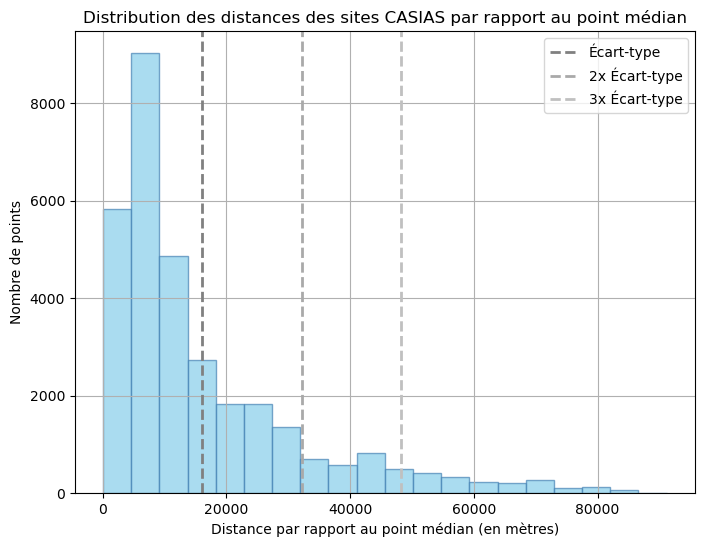
\includegraphics[width=0.75\textwidth]{img/chapitre3/CASIAS_Dispersion_Points_Centraux_1.png} 
\caption{Analyse du nuage de points CASIAS, méthode des distances (1/3)} 
\label{fig:dist_casias_pointmedian_1} 
\end{figure}

La distribution spatiale des sites par rapport au point médian conforte l'analyse de l'écart-type et de la variance, avec une très grande concentration d'anciens sites industriels dans le centre de la métropole parisienne. \textbf{70\% des sites CASIAS se trouvent dans un périmètre de 20km autour du point médian}, soit près de 27 000 sites cumulés. Le graphique \ref{fig:casias_parts_cumulées}) indiquant le nombre cumulé de sites CASIAS depuis le point médian s'approche de très près de la forme d'une courbe exponentielle inverse.  L'analyse par densité du nuage de points complète ce tableau (cf. figure \ref{fig:casias_densités_points}. Les derniers points CASIAS se situant à 80km du point médian, nous avons défini 8 intervalles de distance d'environ 10km chacun. La première tranche de densité (de 0 à 10km environ) domine très largement la distribution des densités. La courbe de distribution des densités est quasi identique à la courbe de distribution des densités.  

La répartition des sites CASIAS semble donc régulière sur le territoire. En analysant le nuage de points par distances et par densités, nous espérions nous affranchir des frontières administratives, discriminant ainsi des sous-groupes géographiques cohérents. Au contraire, cette première étape d'analyse a montré une grande homogénéité dans la répartition spatiale des sites par rapport aux points centraux. La très grande régularité de ces résultats nous surprend, malgré sa grande cohérence avec le système urbain parisien. Les graphiques ne révèlent pas de poches plus denses à distance du centre, pas d'irrégularités dans la distribution. La loi d'agglomération de Clark est confirmée par ces chiffres, et l'hyper centre de la métropole parisienne concentre la grande majorité des sites CASIAS. L'étude de la répartition des sites par commune casse cette image lisse, et nous offre de la matière pour différencier les territoires. 


% Proportion de sites CASIAS selon la distance au point médian (Viz 2 - Graph barres)  
 \begin{figure}[!h] 
\centering  
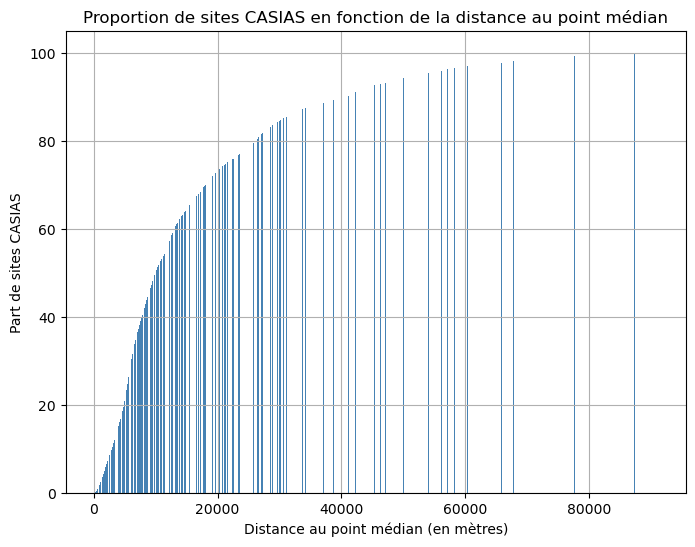
\includegraphics[width=0.4\textwidth]{img/chapitre3/Distribution_Proportion_CASIAS_Point_Median.png} 
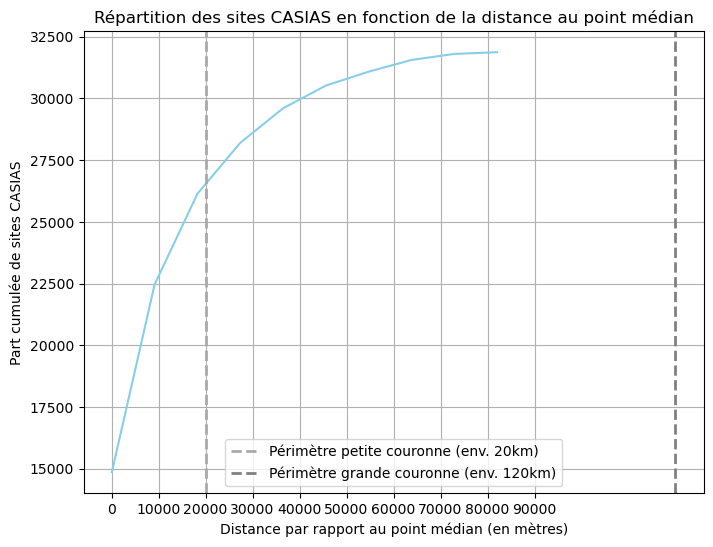
\includegraphics[width=0.4\textwidth]{img/chapitre3/CASIAS_Courbe_Cumulative_Distances_Point_Median.png} 
\caption{Analyse du nuage de points CASIAS, méthode des distances (2/3)} 
\label{fig:casias_parts_cumulées} 
\end{figure}

% Encadré sur les ordres de grandeur
\begin{tcolorbox}[colback=gray!5!white,colframe=gray!20!white]
\textbf{Ordres de grandeurs géographiques en Île-de-France}

La superficie de Paris intramuros est de \textbf{105 km2}, celle des départements de petite couronne hors Paris 657 km2. La zone centrale parisienne cumulée s'étend donc sur 762 km2, selon une \textbf{circonférence} d'environ \textbf{20 km} depuis la cathédrale Notre-Dame de Paris. La superficie totale de l'Île-de-France est de \textbf{12 012 km2}. La distance de la frontière régionale à Notre-Dame varie entre 100 et 150km. Nous choisissons une \textbf{circonférence de 120 km} comme valeur de référence pour l'ordre de grandeur. 
%Par ailleurs, la circonférence maximale de la tâche urbaine continue de la métropole parisienne s'étale jusqu'à 30km depuis le centre de Paris\footnote{Source Atlas du grand Paris}. 
\end{tcolorbox} 

% Proportion de sites CASIAS selon la distance au point médian (Viz 3 - Exponentielle inversée)  
 \begin{figure}[!h] 
\centering  
\includegraphics[width=0.75\textwidth]{img/chapitre3/Proportion_CASIAS_DIST_Pt_Médian_Marqueurs_PC_GC.png} 
\caption{Analyse du nuage de points CASIAS, méthode des distances (3/3)} 
\label{fig:dist_casias_pointmedian_3} 
\end{figure}

% Répartition des densités de points CASIAS
 \begin{figure}[!h] 
\centering  
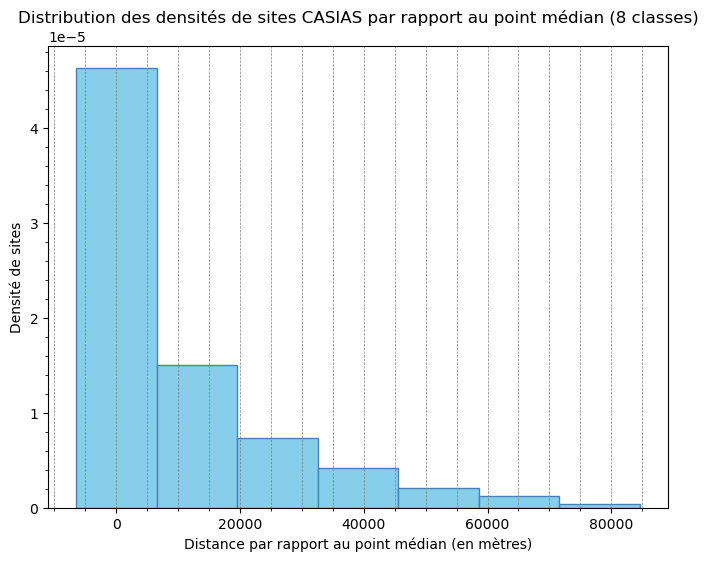
\includegraphics[width=0.75\textwidth]{img/chapitre3/CASIAS_DENSITE_DISTRIBUTION_SITES.png} 
\caption{Analyse du nuage de points CASIAS, méthode des densités} 
\label{fig:casias_densites_points} 
\end{figure}

%%%%%%%
\section{Analyse des points, la question des échelles d'analyse }
%Analyse à la commune
% Encadré vers carte du nb de points CASIAS par commune
\begin{tcolorbox}[colback=gray!5!white,colframe=gray!20!white]
La carte dynamique représentant le \textbf{nombre de sites CASIAS par communes} est disponible sur notre dépôt GitHub : \url{https://charlotte-berthier.github.io/heritages_toxiques/cartes_dynamiques/carte_nb_sites_par_commune.html}
\end{tcolorbox}

La base de données CASIAS nous pose en fin de compte un problème très classique dans l'analyse de données massives : l'abondance de données noie les grandes tendances dans les détails. Il est nécessaire de définir des échelles d'agrégation pertinentes. Pour cette étape, nous avons donc groupé et compté le nombres de sites CASIAS à deux échelles : le département et la commune. L'analyse départementale en nombres absolus n'est pas la plus éclairante. Paris et la Seine-Saint-Denis sortent certes en premier, en cohérence avec leur histoire industrielle. Rapportés à la superficie des départements, ces chiffres reflètent mieux les différences d'intensité industrielle. A titre d'exemple, l'Île-de-France compterait 3 sites CASIAS par km2, contre 65 sites par km2 dans Paris intra-muros. La Seine-Saint-Denis concentre 22 sites par km2, contre seulement 1 site par km2 pour la Seine-et-Marne, dont le nombre absolu de sites est pourtant supérieur. 

L'analyse par commune est la plus intéressante pour analyser les différenciations territoriales. Nous voyons sur la carte \ref{fig:nb_sites_com} qu'une majorité de communes possède peu d'anciens sites industriels. Les 10 communes avec le plus de sites ou anciens sites industriels regroupent à elles seules 5910 sites, soit 19\% de la BDD. Les 20 communes avec le plus de sites ou anciens sites industriels regroupent à elles seules 9457 sites, soit 30\% de la BDD. Les 50 communes avec le plus de sites ou anciens sites industriels regroupent à elles seules 15870 sites, soit 50\% de la BDD. Le graphique \ref{fig:casias_top_communes} montre les communes dénombrant 200 sites CASIAS ou plus, dressant la liste des 36 villes les plus industrielles d'Île-de-France. Chaque arrondissement parisien comptant pour une commune, 16 arrondissements sur 20 figurent sur le graphique. Les grands pôles industriels franciliens ressortent : Montreuil, Saint-Denis et Aubervilliers en tête avec Ivry-sur-Seine, suivis d'Argenteuil, Nanterre, Saint-Ouen, Pantin, Courbevoie, Vitry-sur-Seine, Asnières, Levallois, Issy-les-Moulineaux... La présence de la Seine-Saint-Denis ne nous surprend pas, la zone industrielle de la Plaine-Saint-Denis se trouvant à cheval entre Saint-Denis et Aubervilliers. Le département des Hauts-de-Seine est très représenté dans la liste, plus que le Val-de-Marne, défiant ainsi l'idée préconçue que nous nous faisions des résultats. Avec approximativement 5 000 sites dans chaque département, la Seine-Saint-Denis et les Hauts-de-Seine ont un passé industriel également intense. 

Prenons l'exemple de Boulogne-Billancourt, qui fut une commune d'industrie lourde en même temps que Saint-Denis, et suivant les mêmes tendances d'urbanisation et d'industrialisation (voir chapitre 1). La ville accueillit notamment des industries aéronautiques et automobiles au \siecle{XX}. Employant 30 000 ouvriers sur un site de 11 hectares, l'ancienne usine Renault de l'île Seguin était la plus grande de France. Des années 1930 aux années 1970, l'usine est l'emblème industriel de la démocratisation de la voiture, avec 1 million de 4L produites annuellement dans les années 1960\footnote{Source : Groupe Renault, \url{https://www.renaultgroup.com/news-onair/actualites/lile-seguin-lecrin-historique-de-renault/}}.  L'usine désaffectée est démolie en 2005, douze ans après sa fermeture. L'île Seguin a été réhabilitée en espace culturel et paysager, intégré dans le projet plus large de rénovation urbaine \og{} Île Seguin Rives de Seine\fg{}. L'ancien quartier ouvrier historique du Trapèze est transformé en \og{} ville-parc \fg{}\footnote{Source : Eco-quartier Île-Seguin-Rives-de-Seine, \url{https://www.ileseguin-rivesdeseine.fr/fr/le-quartier-du-trapeze}}, éco-quartier moteur de la gentrification de la zone. Cet exemple nous montre la divergence des destins territoriaux entre Saint-Denis et les anciennes villes industrielles des Hauts-de-Seine, où les populations ouvrières semblent avoir été remplacées plus vite par des populations plus aisées, et où les anciens sites industriels ont fait plus rapidement l'objet de réaménagements. Alors que Saint-Denis abrite encore une majorité de populations défavorisées, Boulogne-Billancourt désindustrialisée devient une banlieue résidentielle et s'embourgeoise.

En revenant à la carte  \ref{fig:nb_sites_com}, nous observons que Saint-Denis et Aubervilliers ont une concentration d'anciens sites industriels très supérieure aux autres pôles industriels.  Cinq communes de Seine-Saint-Denis concentrent la quasi totalité des sites CASIAS départementaux : Montreuil, Saint-Denis, Aubervilliers, Saint-Ouen, Pantin. Dans les Hauts-de-Seine, l'intensité industrielle est répartie entre plus de communes. Le tissu urbain hérité était moins intensément industriel, ce qui offre une piste d'explication sur la différence d'évolution territoriale accentuée depuis la désindustrialisation. Ces divergences territoriales s'expriment au-dessus de sols pollués, quelle que soit l'évolution démographique des communes. 

% Graphique, nombre de points par département
\begin{figure}[!h]
\centering 
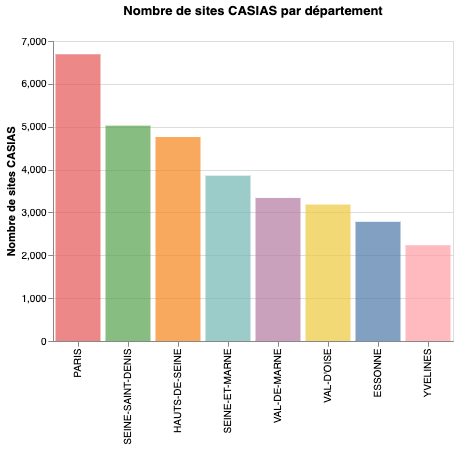
\includegraphics[width=0.75\textwidth]{img/chapitre3/CASIAS_Nb_Sites_par_Dept.png}
\caption{Nombre de sites CASIAS répertoriés par département}
\label{fig:nb_sites_dept_bleu}
\end{figure}

% Carte, nombre de points par département
\begin{figure}[!h]
\centering 
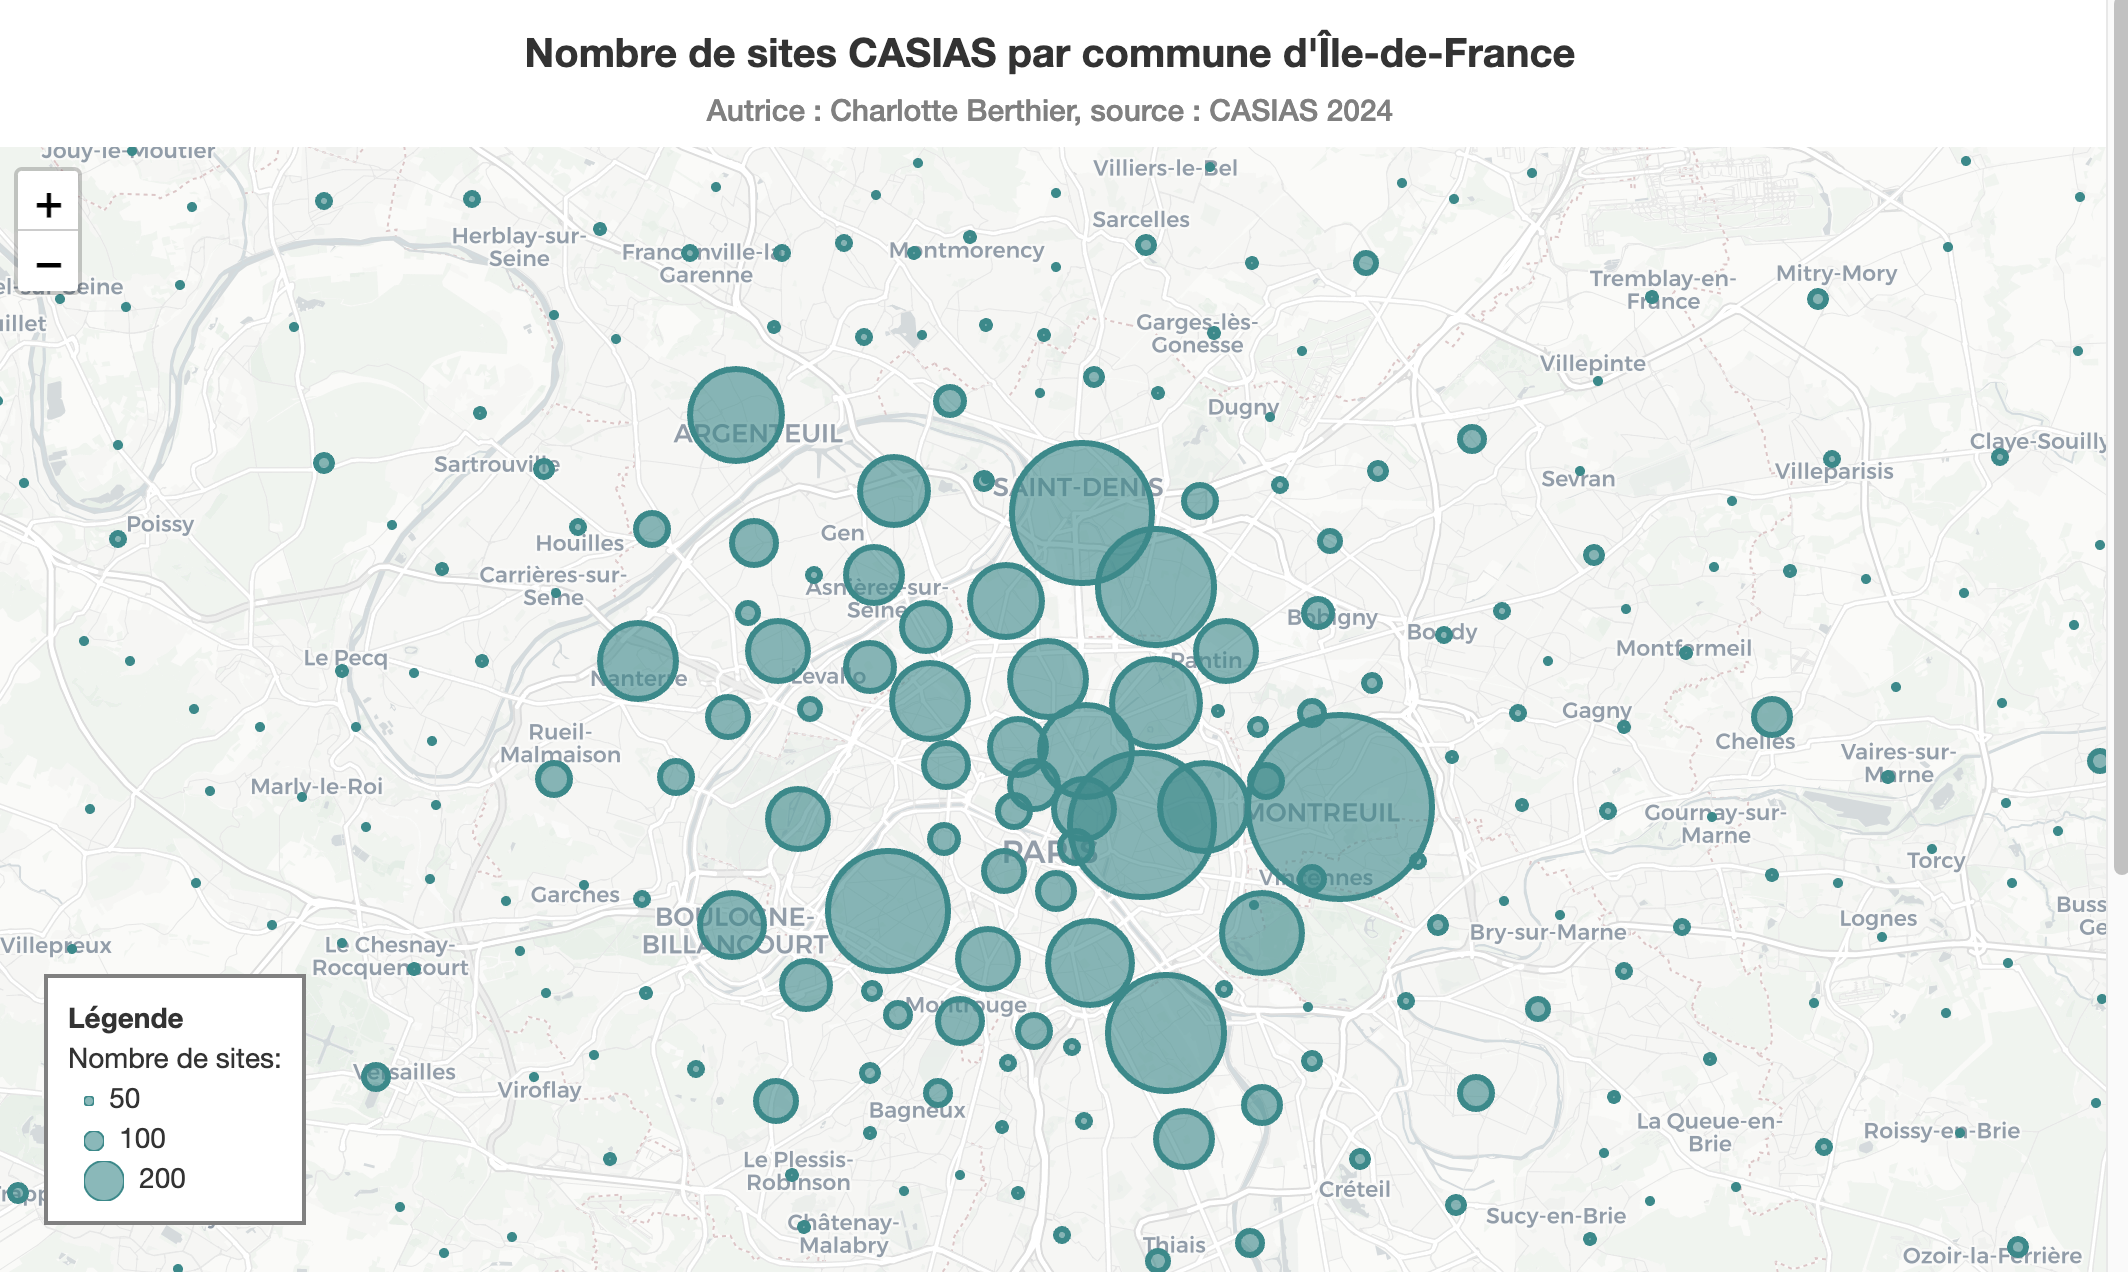
\includegraphics[width=0.75\textwidth]{img/chapitre3/Casias_Carte_Nb_Sites_Com}
\caption{Nombre de sites CASIAS par commune - Extrait de la carte dynamique}
\label{fig:nb_sites_com}
\end{figure}


% Graphique, nombre de points par commune, top 36 communes de plus de 200 points
\begin{figure}[!h]
\centering 
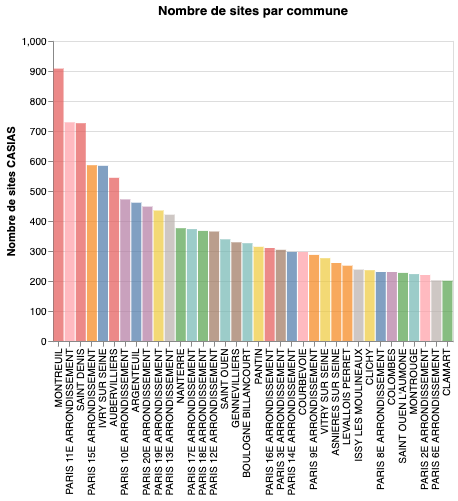
\includegraphics[width=0.75\textwidth]{img/chapitre3/CASIAS_Nb_Sites_par_Commune_Sup200_Top36.png}
\caption{Communes dénombrant plus de 200 sites CASIAS (Top 36)}
\label{fig:casias_top_communes}
\end{figure}

% Carte points pollution moyenne Saint-Denis

\begin{figure}[!h]
\centering 
\includegraphics[width=1\textwidth]{img/chapitre3/Saint-Denis_Moyenne totale}
\caption{Carte de la note moyenne de pollution - Saint-Denis et les communes environnantes}
\label{fig:carte_points_STD}
\end{figure}



\section{Conclusion du chapitre}
%nous ajoutons une nouvelle dimension environnementale à nos modèles d'analyse territoriale. 
En croisant les bases de données CASIAS et ActiviPoll, nous avons reconstitué le système de lieux de l'industrialisation  en Île-de-France, et nous en inférons le système de lieux de la pollution industrielle. Nous avons ainsi confirmé qu'à partir de lieux d'histoire recensés en archives, nous pouvions construire de nouveaux objets socio-environnementaux pertinents.  En prenant en compte la mémoire environnementale attachée aux lieux d'histoire de l'industrie, nous avons donc cherché à comprendre comment la pollution industrielle  se structurait spatialement. L'analyse des données CASIAS ponctuelles nous a permis de dégager de premières structures spatiales à l'échelle régionale. 

L'analyse des points duplicats dans CASIAS nous a permis de mettre en évidence plusieurs phénomènes propres au système spatial industriel en Île-de-France. Dans le centre de Paris, les lieux d'industrie ont une plus forte probabilité de co-présence en un même lieu, ou de succession d'établissements de même type en un même point. Il nous semble que cette structure dans nos données est liée à une proto-industrialisation et une industrialisation très anciennes dans l'enceinte de la ville. Cette co-présence industrielle s'inscrit dans un tissu urbain dense caractérisé par la mixité des usages des sols. En petite et grande couronne, la co-présence de sites témoigne d'un fait territorial plus tardif : la zone industrielle périurbaine séparée du reste de la ville, juxtaposée aux zones résidentielles sans s'y confondre. 

L'analyse par dispersion et par densité du nuages de points nous a par ailleurs confirmé que l'implantation des lieux d'histoire de l'industrie en Île-de-France suit la loi d'agglomération de Clark. A l'échelle régionale, un vaste espace central de pollution se détache en plein coeur de la métropole, intégrant Paris et les communes de petite couronne sur un rayon de 16 à 20km depuis les Halles. Cette zone centrale recoupe de près la zone urbaine continue de Paris, et concentre 80\% des anciens sites industriels de la région. Au-delà de 20km, une rupture s'observe dans les données : la pollution industrielle est diffuse dans toute l'Ile-de-France, mais aiguë dans le coeur de la métropole. Cette répartition semble se maintenir sur l'ensemble des groupes et sous-groupes de substances. 

L'analyse par points nous a permis d'identifier les macro structures régionales du système de lieux de la pollution industrielle. Au sein de la zone centrale où les sites pollués se concentrent, nous cherchons à présent à repérer des sous-ensembles spatiaux cohérents. Pour cela, nous avons dû construire une stratégie d'étude de la pollution à différentes échelles. Il nous fallait passer du point à l'étendue. 


%%%%%%%%%%%%%%%%%%%%%%%%%%%%%%%%%%%%%%%%%%%%%%%%%%%%%%%%%%%%%%%%%%%%%%%%%%%%%
%%%%  PARTIE 2  %%%% Je pense supprimer les parties
% \part{L'étendue des dégâts : les régimes spatiaux de pollution industrielle à Saint-Denis et en Île-de-France}

%% CHAPITRE 4 %%
\chapter{Lieux de pollution, étendue des dégâts : modéliser les hypothèses de pollution industrielle en Île-de-France}
\markboth{\MakeUppercase{\textsc{Chapitre 4. Lieux de pollution, étendue des dégâts}}}{}

\lettrine{L}{a} pollution industrielle ne reste pas confinée en un point, elle se diffuse dans les milieux qu'elle contamine. Cette diffusion dans l'air, l'eau et les sols dépend de la durée, de l'intensité d'exposition et du type de substances relâché dans l'environnement. Sans données quantitatives, il ne nous était pas possible d'appliquer des modèles de diffusion des polluants. Pour approcher la structure spatiale de la pollution industrielle en Île-de-France il était nécessaire de passer d'hypothèses de pollution ponctuelles à une modélisation continue des espaces pollués. Nous cherchions ainsi à approcher la réalité spatiale de la contamination des milieux. Nous cherchions également à mettre en évidence des différenciations territoriales à différentes échelles, l'analyse du nuage de points n'ayant pas fait émerger des sous-espaces évidents de pollution industrielle. Nous avons donc exploré deux modèles spatiaux pour figurer l'étendue de la pollution industrielle en Île-de-France : le \textbf{quadrillage} et la \textbf{carte de chaleur}. 


\section{Le quadrillage}

Afin de trouver la modélisation en quadrillage la plus significative, nous avons fait varier deux paramètres : l’échelle de l’objet spatial de référence, et les méthodes de calcul des hypothèses de pollution. Nous avons exploité pour cela les méthodes numériques de deux articles parus récemment sur l'analyse spatiale de phénomènes socio-historiques. L'article de 2008 \og{} La question des échelles en géohistoire. Les bureaux de la poste aux lettres du XVIIIe siècle à nos jours \fg{} de Ludovic Chalonge et Nicolas Verdier\footnote{\cite{verdier_question_2018}} traite de l'expansion de la couverture spatiale des bureaux de postes. L'article de mars 2024 de Mathilde Basuyau, Laure Chabalier et Philippe Branchu \og{} Développement d'un indice spatialisé de pollution potentielle en éléments traces métalliques des sols urbains en Île-de-France \fg{}\footnote{\cite{charvet_sols_2024}, chapitre 5}, que nous avions cité précédemment, exploite les bases CASIAS et ActiviPoll pour étudier la pollution des sols en Île-de-France. Nous avions déjà commencé nos travaux sur la base CASIAS avant de découvrir l'existence de cet article. Cela nous a offert la possibilité de comparer les méthodes que nous élaborions avec les résultats de l'article. Nous employons toujours le même déroulé méthodologique pour tester les différentes échelles de grille : 

\begin{itemize}
\item Implémentation d’un objet spatial de référence, la grille, permettant d’agréger les données à différentes échelles et de les comparer. Nous cherchons à trouver l’objet spatial le plus significatif pour étudier la pollution des sols. 
\item Agrégation des anciens sites industriels à cette échelle, via une intersection spatiale
\item Somme du nombre de points
\item Somme du nombre de substances
\item Calcul des hypothèses de pollution (agrégation des notes à l'échelle de la grille)
\end{itemize}

Pour cette dernière étape, nous avons comparé deux méthodes de calculs différentes, suite à la lecture de l'article de M. Basuyau et \textit{alii}. Nous avions initialement prévu de simplement calculer la valeur moyenne de pollution. L'article propose une méthodologie plus élaborée en construisant un \og{} indice de pollution potentielle \fg{}. 

\subsection{Méthode 1 - Les notes moyennes d'hypothèses de pollution}
Nous avons déjà décrit cette étape dans la présentation de notre chaîne de traitement  (voir sous-partie 3.1.4). Afin de faciliter la comparaison avec la deuxième méthode, voici un rappel de notre méthode de calcul des notes moyennes de pollution : 
\begin{itemize}
\item Chaque site CASIAS a une note entre 0 et 8 pour chaque sous-groupe de substances, correspondant à sa probabilité de pollution à cette sous-substance
\item Pour chaque site CASIAS, nous avons reconstitué la probabilité de pollution des six groupes de polluants d'ActiviPoll, en calculant la moyenne arithmétique des sous-groupes qui leur étaient associés
\item Pour chaque taille de quadrillage, nous intersectons les carreaux et les points. Puis pour chaque carreau nous calculons la note moyenne de pollution des sous-groupes de substances en faisant la moyenne arithmétique des notes de tous les points. La note des six groupes est recalculée à partir des notes moyennes des sous-groupes, ainsi que le nombre de substances présentes. 
\end{itemize}

\subsection{Méthode 2 - L'indice de pollution potentielle (IPP)}

\begin{quote}
\og{} L'indice de pollution potentielle vise à hiérarchiser les sols urbains franciliens selon un niveau potentiel de pollution établi en l'absence de données physico-chimiques accessibles. \fg{}
\end{quote}

L'IPP est construit comme un indice à notation. L'indice maintient ainsi le format initial des données d'ActiviPoll, qui attribuait une note de probabilité à chaque substance. Chaque carreau de la grille se voit \og{}affecter deux notes qui renvoient à des classes de valeurs définies à dire d'expert\fg{}\footnote{\cite{charvet_sols_2024}, page 82}. La première note décrit le nombre de sites CASIAS présents dans le carreau. La seconde note caractérise le niveau de pollution potentielle. La valeur finale du carreau correspond au produit normalisé de ces deux notes, discrétisé en plusieurs classes par la méthode des seuils naturels de Jenks. Nous avons utilisé une normalisation min max pour ramener toutes les valeurs entre 0 et 1. 

% Schémas calcul IPP 
\begin{figure}[!h]  
\centering   
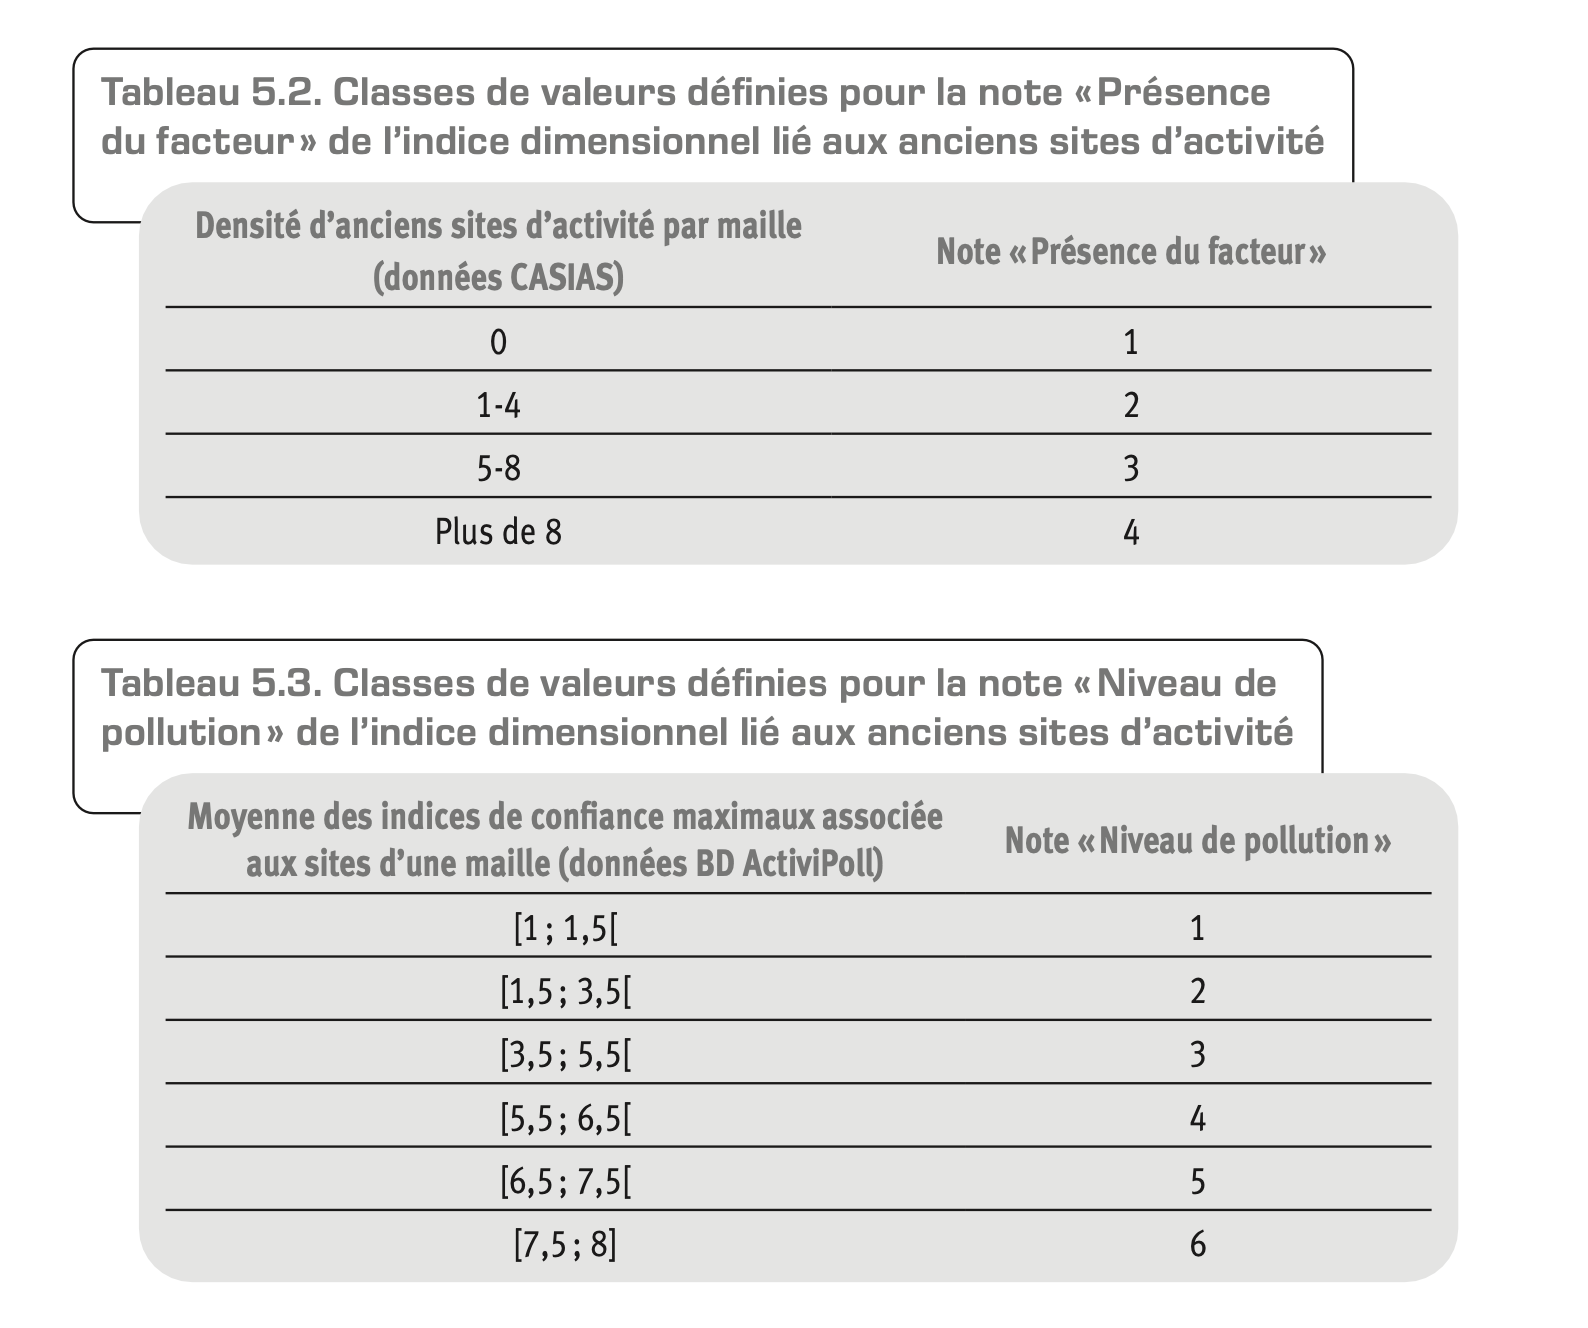
\includegraphics[width=0.75\textwidth]{img/chapitre4/IPP_2_Notes} 
\hspace{0.05\textwidth}
\includegraphics[width=0.75\textwidth]{img/chapitre4/IPP_Schéma} 
\caption{Méthode de calcul de l'indice de pollution potentiel (IPP)}  
\label{fig:calcul_IPP}   
\end{figure}  

Les deux méthodes produisent des résultats très proches. En comparant les résultats des deux méthodes (voir les tableaux de synthèse en figure \ref{fig:Tableaux_Synth_Carreaux}), on observe que la méthode 1 des moyennes est plus sensible aux valeurs extrêmes que l'approche par l'indice de pollution potentielle. En comparant le nombre de carreaux pour chaque groupe de substances, on voit que l'IPP indique systématiquement un nombre de carreaux légèrement inférieur à celui de la méthode 1. 

\begin{figure}[!h] 
\centering  
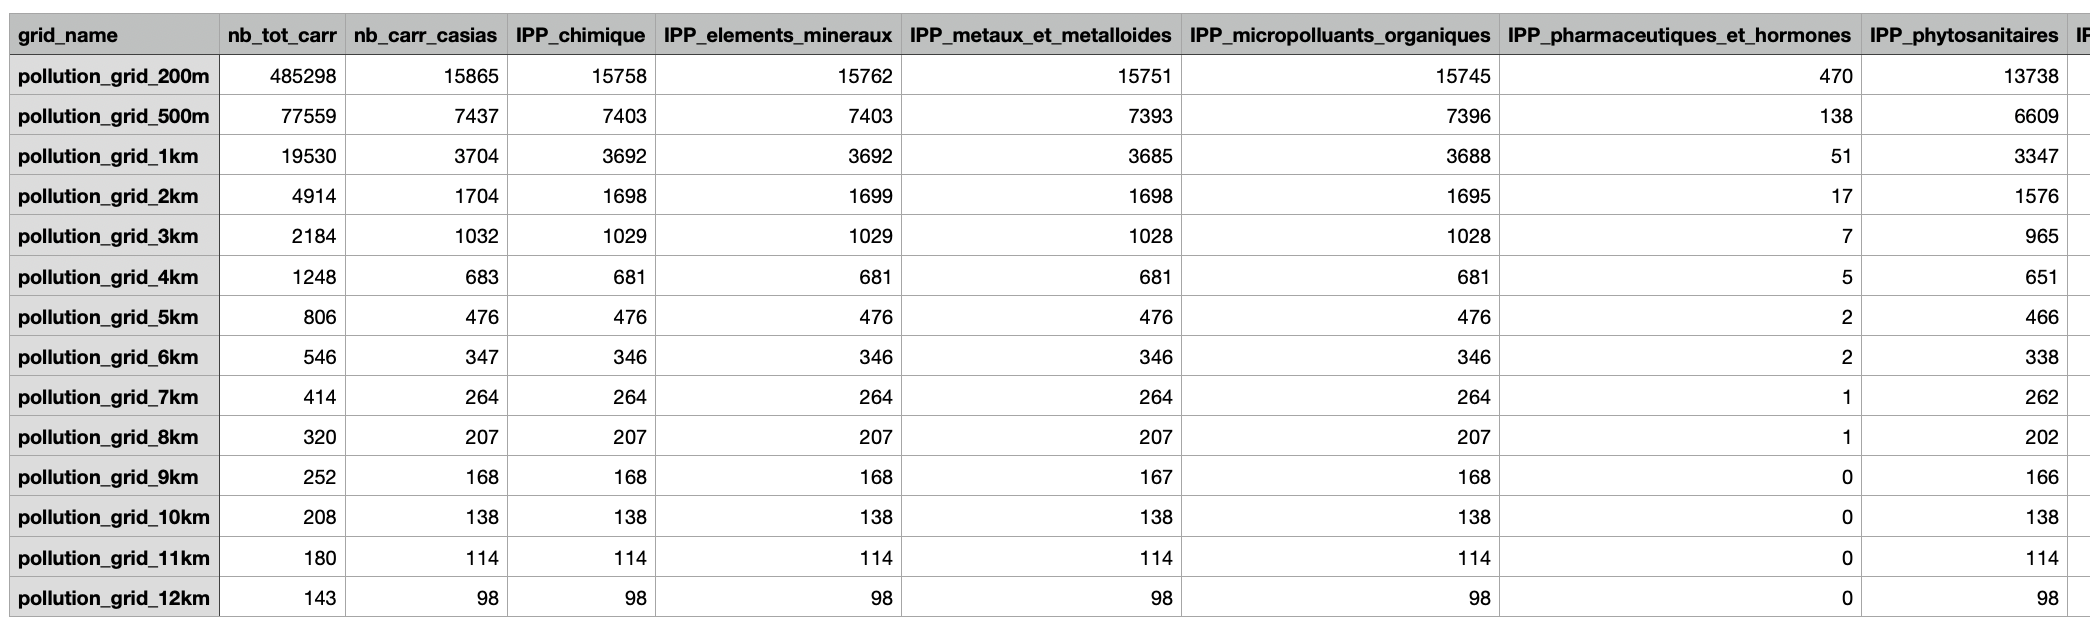
\includegraphics[width=1\textwidth]{img/chapitre4/Methode1_Tableau_Synth_carr.png} 
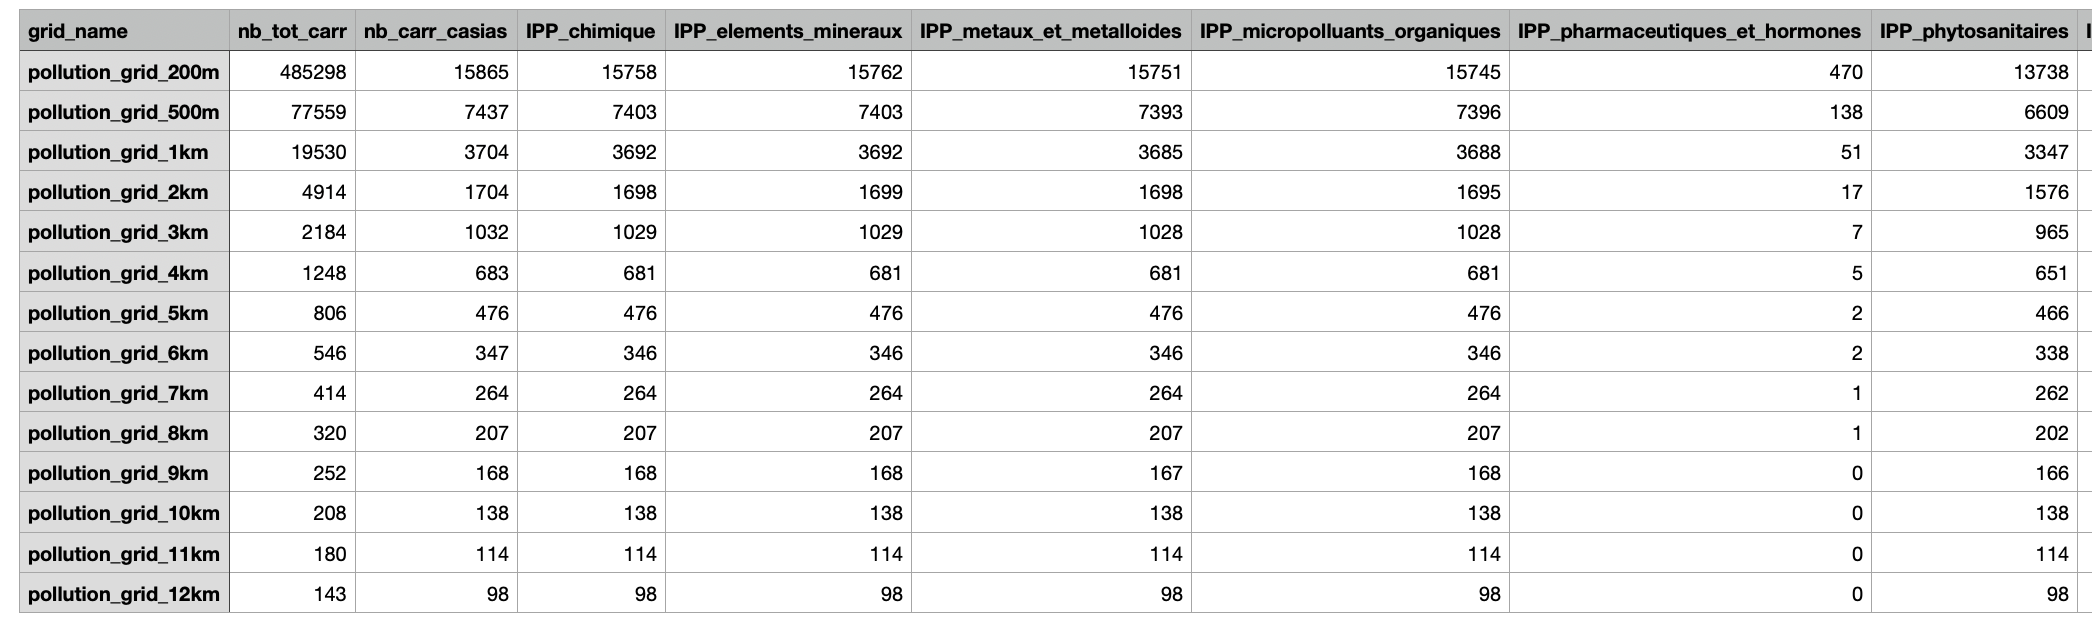
\includegraphics[width=1\textwidth]{img/chapitre4/Methode2_Tableau_Synth_carr.png} 
\caption{Synthèse des hypothèses de pollution par quadrillage - Tableau du haut : méthode 1 (Moyenne),  Tableau du bas :  Méthode 2 (IPP)} 
\label{fig:Tableaux_Synth_Carreaux} 
\end{figure} 

L'IPP atténue donc les effets des valeurs extrêmes dans les notations, et réalise une modélisation des hypothèses de pollution un peu plus prudente dans l'échelle de notation. Ces différences sont cependant ténues. Les valeurs moyennes de la méthode 1 semblent relativement peu affectées par des valeurs extrêmes. Le nombre de carreaux par groupe de substances varie peu entre les deux méthodes, ce qui confirme encore une fois la diffusion importante de la pollution sur le territoire régional. Nous avons choisi de poursuivre nos modélisations en utilisant l'indice de pollution potentielle proposé par M. Basuyau et \textit{alii}. Il nous semblait en fin de compte plus robuste de conserver un indice de notation jusqu'au bout dans l'agrégation des hypothèses de pollution à différentes échelles. Cela convient mieux à l'observation de ces variables qualitatives. La première méthode par moyenne pourrait faire passer nos notations pour des données quantitatives. La normalisation apporte également une lecture plus propre des résultats. 


% Table de description des variables
\begin{table}[h]
\centering
\small
\caption{Agréger les notes de pollution à toutes les échelles : synthèse des méthodes de calcul}
\begin{tabular}{>{\raggedright}p{3.5cm}p{3.5cm}p{2cm}p{3.5cm}}
    \toprule
    Objet géométrique & Calcul & Fiabilité & Notes \\
    \midrule
    Point & Méthode 1 - Moyenne & Bonne & Sensibilité aux valeurs extrêmes : moins de valeurs centrales\\
    Point & Méthode 2 - IPP & Bonne & Plus prudent sur les notes extrêmes : plus de valeurs centrales \\
    Quadrillage & Méthode 1 - Moyenne & Moyenne & Couverture spatiale légèrement plus importante \\
    Quadrillage & Méthode 2 - IPP & Bonne & Couverture spatiale légèrement inférieure \\
    \bottomrule
\end{tabular}
\end{table}


\subsection{Comparaison de quatorze quadrillages}

\og{} Pour calculer l’IPP, seuls les carreaux de la maille Insee intersectant la tache urbaine francilienne (périmètre d’intérêt de l’étude) sont conservés. (page 81)\fg{}

Nous divergeons sur ce point avec la méthodologie proposée dans l'article de M. Basuyau et \textit{alii}. L'utilisation du carroyage INSEE offre l'immense avantage de pouvoir intégrer facilement des données démographiques prêtes à l'emploi dans l'analyse. Mais cela limite le périmètre d'étude, et nous avons souhaité nous affranchir de cette contrainte. Par ailleurs, l'étude de 2024 se concentre sur un seul type de polluants : les éléments traces métalliques (équivalents aux métaux et métalloïdes dans ActiviPoll). Or nous cherchons à monter en généralité dans l'analyse de la pollution industrielle des sols, en intégrant l'ensemble des substances dans l'analyse de sa répartition spatiale. Nous souhaitions expérimenter la construction de méthodes d'analyse regroupant les substances pour parler de la pollution des sols au global. Dès lors, quelle est l'échelle d'analyse pertinente pour comparer les substances entre elles et construire des indicateurs agrégés ? Nous avions besoin de créer une échelle d'analyse transverse à tous les groupes de substances (nous n'avons pas traité les soixante-douze sous-groupes pour cette partie). Nous avons donc reproduit la méthodologie employée par N. Verdier et L. Chalonge dans leur article sur les bureaux de postes. En utilisant le langage R, nous avons créé quatorze quadrillages différents, allant de l'échelon infra-urbain le plus fin (200 mètres), à l'échelle d'un regroupement de communes (12 kilomètres).  Nous pouvions ainsi explorer nos données à l'échelle infra-urbaine, urbaine et inter-urbaine selon plusieurs niveaux de finesse. 

% Table des échelles de quadrillage
\begin{table}[h]
\centering
\small
\caption{Échelles de quadrillage calculées}
\label{fig:14_grilles}
\begin{tabular}{>{\raggedright}p{3.5cm}p{3.5cm}p{5cm}}
    \toprule
    Taille des carreaux & Échelle & Équivalence spatiale \\
    \midrule
    200m & Infra-urbaine & Voisinage (îlots proches) \\
    500m & Infra-urbaine & Quartier proche \\
    1km & Infra-urbaine & Quartier \\
    2km & Infra-urbaine & Quartier élargi \\
    3km & Urbaine & Arrondissement, Commune  \\
    4km & Urbaine & Commune \\
    5km & Urbaine & Commune \\ 
    6km & Inter-urbaine & Plusieurs communes \\
    7km & Inter-urbaine & Plusieurs communes\\
    8km & Inter-urbaine & Plusieurs communes\\
    9km & Inter-urbaine & Plusieurs communes\\
    10km & Inter-urbaine & Plusieurs communes\\
    11km & Inter-urbaine & Plusieurs communes\\
    12km & Inter-urbaine & Plusieurs communes\\
    \bottomrule
\end{tabular}
\end{table}

La question de la dimension des quadrillages est à prendre en compte dans l’analyse de tout phénomène spatial. Nous cherchions à établir la taille de grille la mieux adaptée pour comparer les espaces de pollution des sols. Sur le modèle de l'article, nous cherchions à comprendre le \og{} rapport à la synthèse que permet ou pas la variation d'échelle \fg{} \footnote{\cite{verdier_question_2018}, page 12}, à  voir si des "moments particulièrement lisibles" apparaissaient dans les données en faisant varier l'échelle d'agrégation.  Nous cherchons à réduire l'information contenue dans les points CASIAS pour en extraire des régimes spatiaux de pollution industrielle. Observe-t-on des paliers entre les échelles d'analyse? Quels espaces pollués voit-on apparaître, à quelles échelles ?  Nous passons d'une logique de points de pollution à une logique de couverture spatiale, c'est-à-dire d'exposition à la pollution. 



%Tableaux de synthèse des carroyages 
\clearpage
\begin{figure}[!h] 
\centering  
\includegraphics[width=1\textwidth]{img/chapitre4/CARROYAGE_IPP_CHIMIQUE_200M.png} 
\includegraphics[width=1\textwidth]{img/chapitre4/CARROYAGE_IPP_CHIMIQUE_500M.png} 
\caption{Modélisation de la pollution chimique en Île-de-France, comparaison des carroyages de 200 et 500 mètres} 
\label{fig:carte_IPP_Chimique_200m_500m}
\end{figure} 

\footnote{Les cartes des carroyages 200m et 500m se sont avérées trop lourdes pour le logiciel R Studio. Nous les avons donc réalisées à l'aide du logiciel QGIS. Ceci explique la différence de mise en page avec les quadrillages suivants. L'échelle a été reproduite à l'identique.}

Contrairement à la méthodologie originale de l'article, nous ne prenions pas en compte une variabilité temporelle, mais la variation spatiale d'un phénomène physique. Nous cherchions à connaître la proportion de carreaux potentiellement pollués selon les groupes de substances et selon la taille des carreaux. Nous voulions savoir si des espaces de pollution des sols différents apparaissaient selon les groupes de substances. Les figures \ref{fig:carte_IPP_Chimique_200m_500m}, \ref{fig:carte_carroyages_IPP_Chimique_1} et \ref{fig:carte_carroyages_IPP_Chimique_2} cartographient l'indice de pollution potentiel aux polluants chimiques en Île-de-France, pour les quatorze grilles créées. A partir de 3km de carreau, les quadrillages perdent en intérêt : ils sont trop larges. L'agrégation de nombreux points dans des carreaux trop grands empêche de distinguer les variations territoriales de la pollution des sols. La zone centrale très dense émerge à nouveau, et les valeurs de l'indice de pollution sont tirés vers le bas. On constate à nouveau une pollution diffuse, d'une probabilité moyenne. Le quadrillage de 12km ne distingue plus grand chose. Les points très pollués aux confins de l'Île-de-France correspondent à des zones où il y a très peu de points CASIAS, donc où la note d'IPP est moins tirée vers le bas qu'ailleurs (voir le carreau centré sur Chaussy/Omerville par exemple). Les quadrillages infra-urbains sont les plus intéressants pour différencier les espaces de pollution des sols, particulièrement les quadrillages de 200m, de 500m et d'1km. 

La pollution des sols aux produits pharmaceutiques et aux hormones est la contamination la moins courante en Île-de-France. Elle se détache très facilement des autres groupes. Les cinq autres groupes de substances sont présents dans les mêmes proportions en Île-de-France, nous ne distinguons pas de géographie spécifique à un groupe de substances. Il faudrait sans doute combiner l'analyse des soixante-douze sous-groupes de substances et une analyse sectorielle de l'industrie pour découvrir des variations plus significatives. Pour les six groupes de substances, des variations d'intensité du potentiel de pollution sont observables, mais selon une répartition géographique globalement homogène entre les groupes. A partir du quadrillage de 1km, nous différencions clairement des espaces de pollutions en Île-de-France. Le passage aux échelles 500m puis 200m affine ces zones sur la carte, en progressivement de l'échelle du quartier à celle du quartier proche jusqu'à celle de l'îlot. Ces zones sont cohérentes avec notre connaissance de l'histoire industrielle de la région.  

Une zone de \textbf{concentration centrale} se détache dans le coeur de la métropole : 
\begin{itemize}
\item Les Halles, le faubourg Montmartre et le faubourg Saint-Antoine se détachent clairement, ainsi que l'ancien XVe arrondissement ouvrier
\item La banlieue immédiate Nord, de Pantin à Levallois avec Saint-Denis au centre, forme une large bande continue et bien identifiée. Elle s'évase vers le Nord le long des axes de circulation traversant la boucle de la Seine au niveau d'Argenteuil. 
\item Montreuil se détache à l'Est, mais n'est pas en continuité complète avec la banlieue Nord
\item La banlieue immédiate Sud, de Boulogne jusqu'à Ivry-sur-Seine et Vitry-sur-Seine. Cette zone est plus étroite que dans le Nord.  
\end{itemize}

On observe ensuite une dispersion de la pollution des sols en grande couronne, le long des axes de circulation et autour des pôles urbains régionaux : 
\begin{itemize} 
\item Chilly-Mazarin
\item Evry
\item Mantes-la-Jolie
\item Melun 
\item Meaux 
\item Mitry-Mory (aéroport Charles-de-Gaulle)
\item Orly
\item Persan
\item Pontoise 
\item Rungis
\item Etc.  
\end{itemize}

Lors de la création des quatorze grilles, nous avons généré un tableau de synthèse pour toutes les substances et tous les quadrillages (voir figure \ref{fig:Tableaux_Synth_Carreaux}). Cela nous a permis de réaliser un graphique figurant la variation du nombre de carreaux pollués selon l'échelle géographique. Mis à part la courbe de la pollution pharmaceutique, presque égale à zéro, les courbes de la pollution totale et des six grands groupes de substances se confondent presque parfaitement. Cela indique que les répartitions spatiales des différents polluant sont identiques. En somme, la modélisation par quadrillage n'est pas concluante pour modéliser et distinguer différents espaces de pollution en fonction des types de polluants. La figure \ref{fig:graph_carroyages} permet de mieux voir les six courbes de forme identique. 

\begin{figure}[!h] 
\centering  
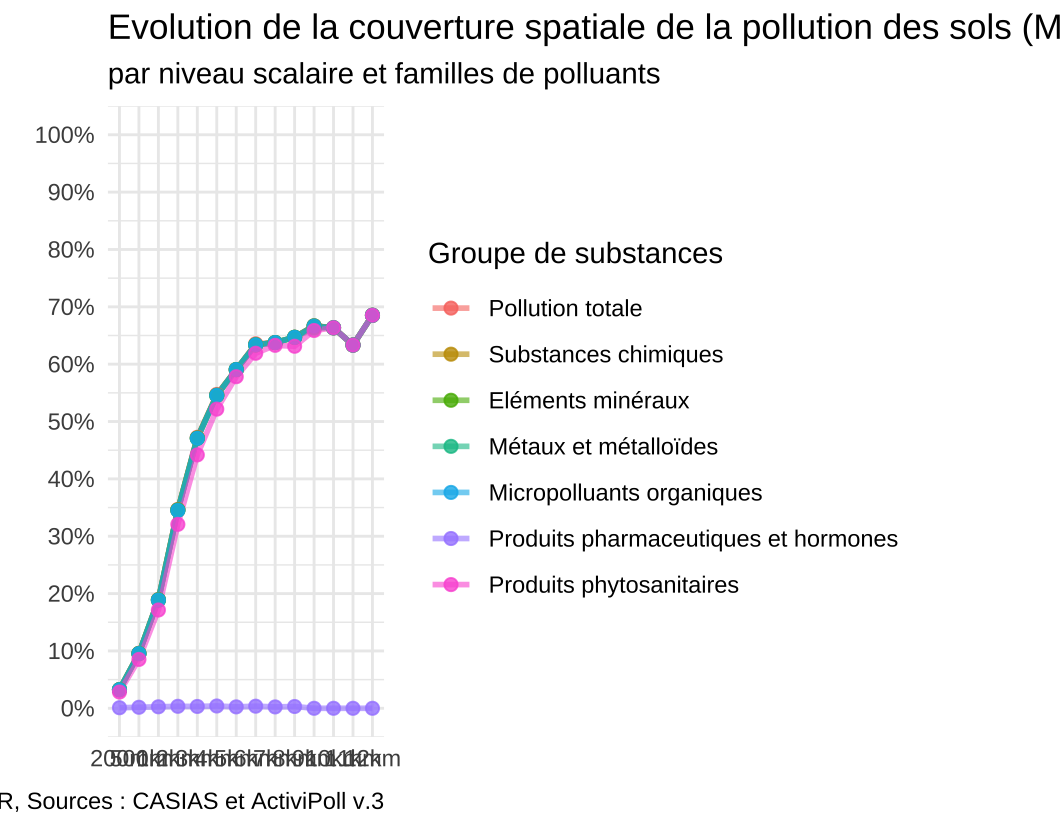
\includegraphics[width=0.75\textwidth]{img/chapitre4/Graphique_Evo_Couv_Spa_Carreaux_1graph.png}
\caption{Graphique synthétique - Evolution de la couverture spatiale de la pollution des sols selon la taille de quadrillage} 
\label{fig:graph_evo_couv_1graph}
\end{figure} 

\clearpage
%\vspace*{2cm}
\begin{figure}[!h] 
\centering  
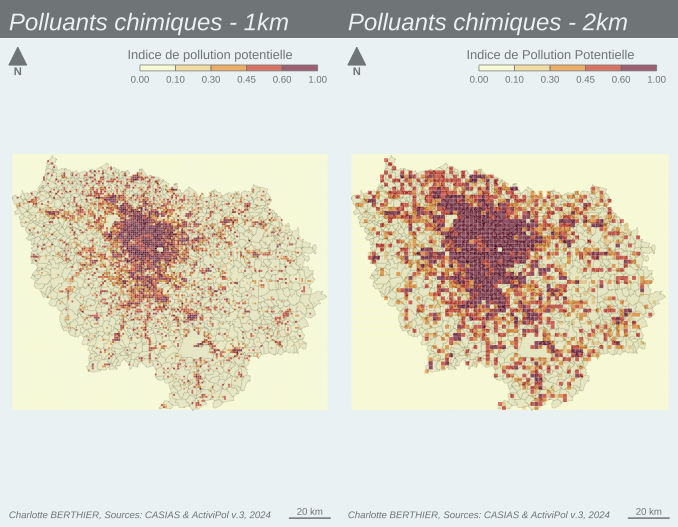
\includegraphics[width=0.75\textwidth]{img/chapitre4/CARROYAGE_IPP_CHIMIQUE_1KM_2KM.png}
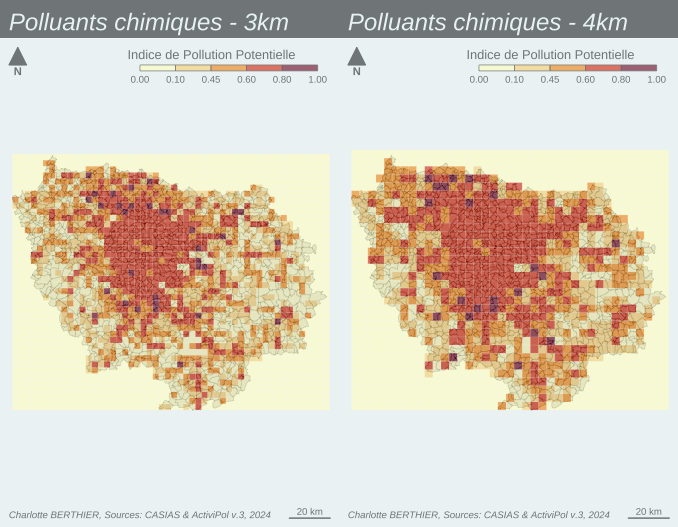
\includegraphics[width=0.75\textwidth]{img/chapitre4/CARROYAGE_IPP_CHIMIQUE_3KM_4KM.png}
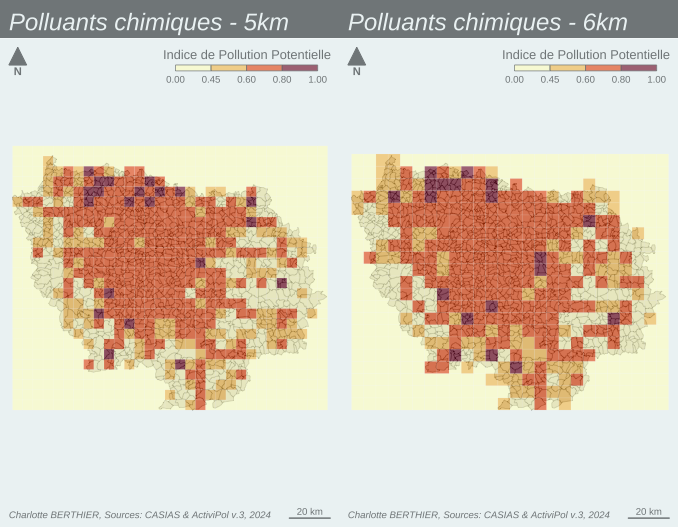
\includegraphics[width=0.75\textwidth]{img/chapitre4/CARROYAGE_IPP_CHIMIQUE_5KM_6KM.png}
\caption{Modélisation de la pollution chimique en Île-de-France, comparaison des carroyages de 1km à 6km} 
\label{fig:carte_carroyages_IPP_Chimique_1}
\end{figure} 

\clearpage
%\vspace*{2cm}
\begin{figure}[!h] 
\centering  
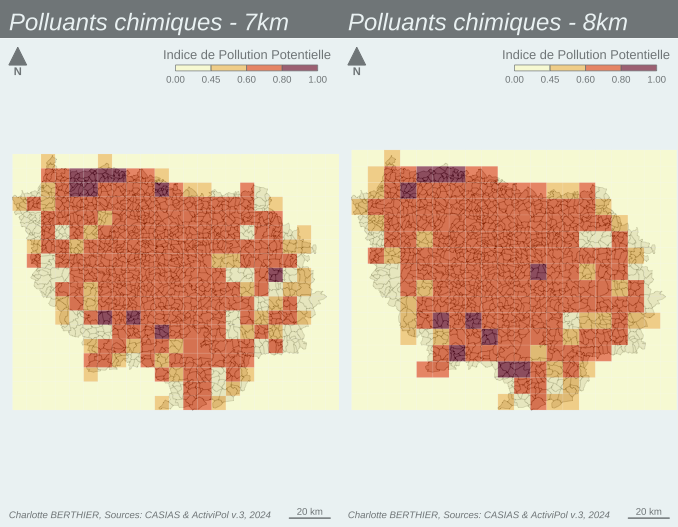
\includegraphics[width=0.75\textwidth]{img/chapitre4/CARROYAGE_IPP_CHIMIQUE_7KM_8KM.png}
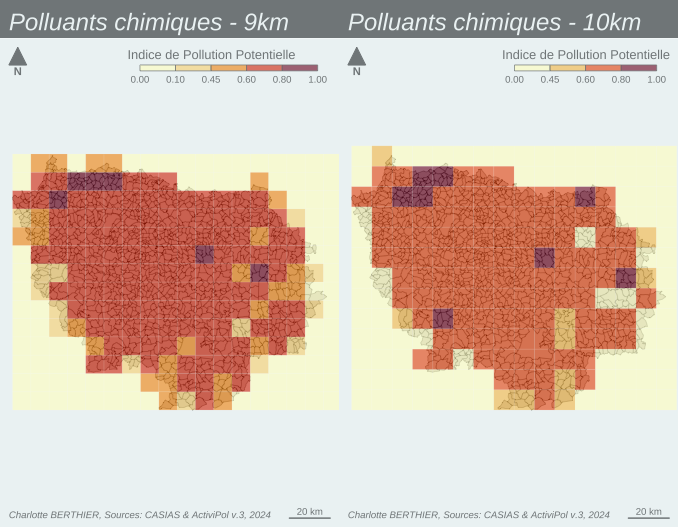
\includegraphics[width=0.75\textwidth]{img/chapitre4/CARROYAGE_IPP_CHIMIQUE_9KM_10KM.png}
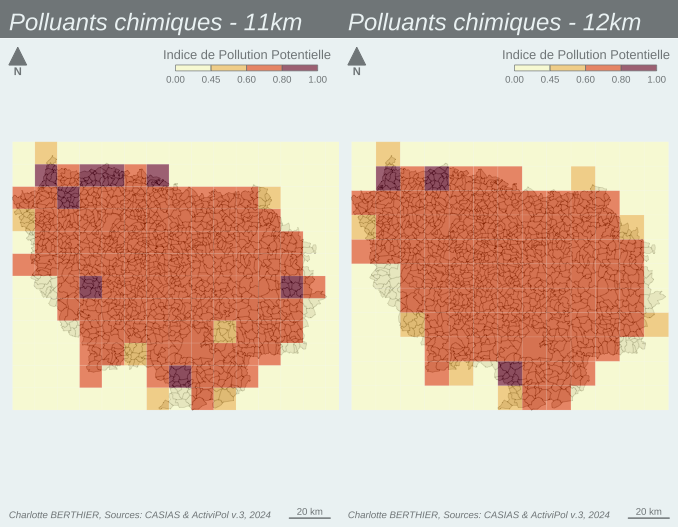
\includegraphics[width=0.75\textwidth]{img/chapitre4/CARROYAGE_IPP_CHIMIQUE_11KM_12KM.png} 
\caption{Modélisation de la pollution chimique en Île-de-France, comparaison des carroyages de 7km à 12km} 
\label{fig:carte_carroyages_IPP_Chimique_2}
\end{figure} 

% Graphique - Evolution de la couverture spatiale de la pollution des sols selon la taille de carroyage 
\clearpage
\vspace*{2cm}
\begin{figure}[!h] 
\centering  
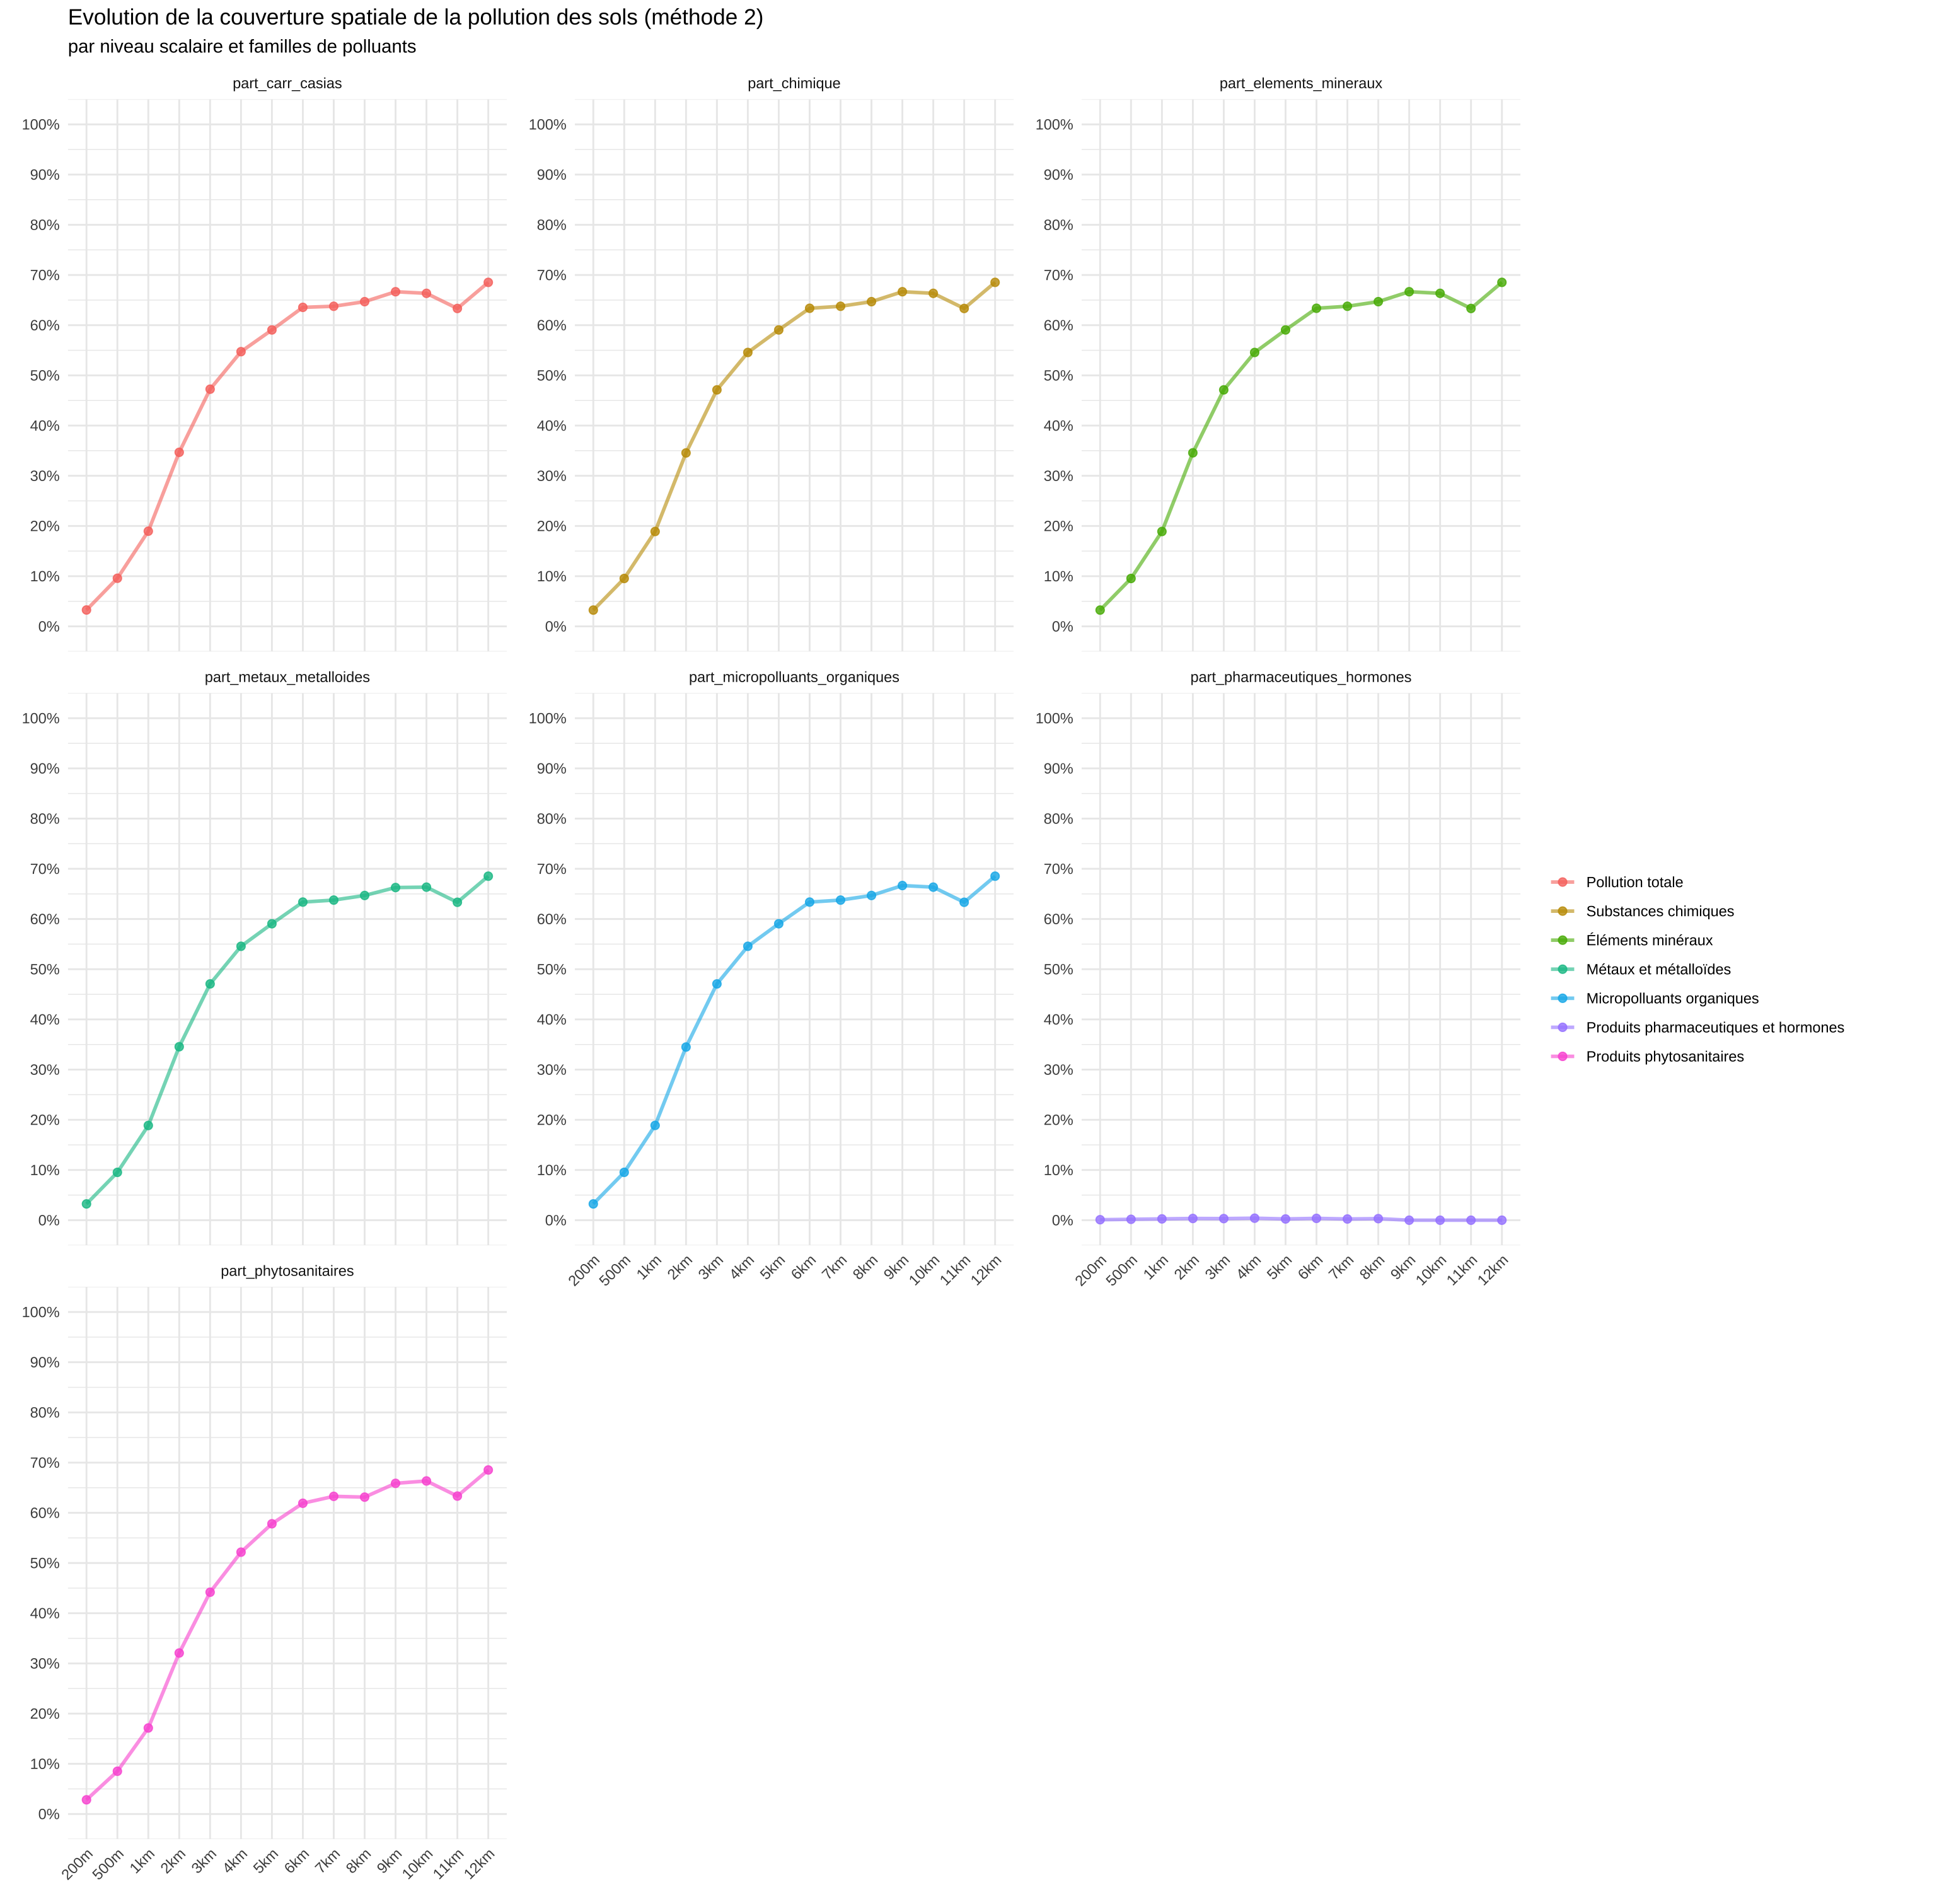
\includegraphics[width=1.3\textwidth]{img/chapitre4/Methode2_Graph_Evo_couv_spa_pol_sols_6groupes_facettes.png} 
\caption{Graphique détaillé - Evolution de la couverture spatiale de la pollution des sols selon la taille de quadrillage} 
\label{fig:graph_carroyages}
\end{figure} 



\section{Cartes de chaleurs}

Nous avons ensuite réalisé des cartes de chaleur pour modéliser la pollution des sols, en utilisant un modèle de Kernel Density Estimation (KDE). La méthode de densité de noyau permet d'estimer la densité de points sur une surface géographique. Elle est couramment utilisée en analyse spatiale pour réaliser des cartes de chaleur, permettant d'identifier les zones concentrant un phénomène. La méthode de densité de noyau fonctionne en lissant la distribution spatiale des points sur une surface continue. Chaque point de données est entouré par une fonction de noyau qui attribue une densité non nulle aux points voisins, créant ainsi une surface de densité lisse.

Nous avons réalisé la dernière étape de notre analyse spatiale sur QGIS\footnote{Version 3.34.2-Prizren} plutôt que sur R, afin d'accélérer la production des dernières cartes. Nous avons utilisé la fonction Heatmap, une fonction d'interpolation spatiale implémentée dans QGIS\footnote{Nom de l'algorithme dans la documentation QGIS : qgis:heatmapkerneldensityestimation }. A partir de notre couche de points CASIAS, un raster de densité est calculé grâce à cet algorithme. Les points chauds de la base sont calculés en fonction d'un nombre de points présents en un même lieu, puis pondérés en fonction d'une variable cible. La figure \ref{fig:heatmap_nb_substances} montre par exemple la carte de chaleur des sites CASIAS pondérée par le nombre de substances polluantes présentes dans les sols. 

La modélisation de la pollution par carte de chaleur nous a semblé la plus pertinente pour étudier la pollution toutes substances confondues. Les cartes de chaleur étant créées à partir des points, elles conservent le même niveau de fiabilité statistique que ceux-ci. Nous créons les cartes de chaleur directement à partir des points, sans avoir à les agréger comme nous avions dû le faire pour les grilles. Nous évitons ainsi la dilution de la probabilité de pollution. Cela nous permet de réaliser des cartes de chaleurs des deux indicateurs englobants que nous avions construits : la pollution moyenne et le nombre de substances. La carte de chaleur est intéressante aussi aux échelles locales et régionales. A l'échelle régionale, les macrostructures identifiées à chaque étape de notre étude, zone centrale très polluée et gradient de diffusion vers le reste de l'Île-de-France, sont bien visibles. A l'échelle locale, l'adaptation de l'échelle permet d'éliminer les valeurs extrêmes de la zone centrale, et donc d'observer les phénomènes locaux de concentration de pollution des sols. Les contours adaptatifs de la carte de chaleur s'adaptent bien à nos données qualitatives de probabilité de pollution des sols. 

La carte de chaleur \ref{fig:heatmap_m_totale} se concentre sur Saint-Denis et la banlieue industrielle Nord. Nous avons pondéré cette carte de chaleur avec la moyenne de pollution. La zone industrielle de La Plaine-Saint-Denis se détache très nettement, particulièrement dans la zone immédiatement au Sud des rails du RER B actuel, et le long de l'axe routier Avenue du Président Wilson / autoroute A1 en direction de Paris.  Cette zone a concentré les industries lourdes les plus polluantes de la zone, jusqu'au Stade de France. Les autres zones rouges correspondent à l'ancienne étendue industrielle de Seine-Saint-Denis. 

% Encadré sur les KDE 
\begin{tcolorbox}[colback=gray!5!white,colframe=gray!20!white]

Un noyau (kernel) est une fonction statistique de pondération. Le Kernel Density Estimation estime la densité d'une variable aléatoire, et la probabilité de l'observer à partir d'un point. Pour réaliser nos cartes, nous avons utilisé le noyau d'Epanechnikov, ou noyau parabolique.  Ce noyau permet d'avoir l'estimateur le plus efficace pour analyser la densité\footnote{Nous suivons la recommendation de la documentation QGIS sur ce point}
\end{tcolorbox}


\begin{figure}[!h]
\centering 
\includegraphics[width=1\textwidth]{img/chapitre4/Heatmap_substances_IDF.png}
\caption{Carte de chaleur, sites CASIAS pondérés par le nombre de substances à Saint-Denis et dans les communes environnantes}
\label{fig:heatmap_nb_substances}
\end{figure}

\begin{figure}[!h]
\centering 
\includegraphics[width=1\textwidth]{img/chapitre4/Heatmap-SaintDenis_M_totale.png}
\caption{Carte de chaleur, sites CASIAS pondérés par le nombre de substances à Saint-Denis et les communes environnantes}
\label{fig:heatmap_m_totale}
\end{figure}

\section{Conclusion du chapitre}

A partir de l’étude des lieux d’histoire de l’industrie, nous avons cherché à reconstituer les régimes spatiaux de la pollution industrielle. Nous cherchions ainsi à mettre en évidence l’organisation spatiale de la pollution industrielle en Île-de-France. Pour ce faire, nous avons utilisé une méthode de calcul par indices de notation, l'indice de pollution potentielle. Cela nous a ensuite permis d'agréger les données CASIAS dans quatorze quadrillages différents. Les échelles les plus pertinentes d'analyse de la pollution des sols sont les échelles infra-urbaines, aux mailles 200m, 500m et 1km. Ces échelles permettent de distinguer finement les anciens espaces industriels franciliens. 

En revanche, les espaces pollués ainsi modélisés ne semblent pas varier selon les groupes de polluants. Deux hypothèses sont envisageables. Soit la pollution industrielle de la zone centrale est telle qu'aucune distinction de substances ne peut affiner la géographie des espaces pollués. Soit les six grands groupes de substances ne sont pas assez précis pour permettre des distinctions spatiales. Nous privilégions la première hypothèse, mais il faudrait poursuivre notre étude par l'investigation d'un secteur industriel précis et des sous-groupes de substances pour le confirmer.

Les cartes de chaleurs sont les plus intéressantes pour obtenir une vision globale de la pollution des sols, par l'intermédiaire des indicateurs globaux de pollution que nous avons créés : la pollution moyenne et le nombre de substances. Le carroyage convient mieux pour l'analyse de la pollution potentielle de chaque groupe et sous-groupe de substances.

En l'état, ces deux essais de modélisation confirment que les anciens sites industriels CASIAS peuvent être définis comme autant de briques élémentaires d'analyse infra-urbaine de l'état environnemental de la métropole parisienne\footnote{\cite{gravier_deux_2018}, Sur le modèle d'analyse infra-urbaine proposé par Julie Gravier }.

%%%%  CONCLUSION  %%%%
\chapter*{Conclusion}
\addcontentsline{toc}{chapter}{Conclusion}

\lettrine{A}{nalyser} spatialement la pollution, c'est tracer les contours d'un espace de risque socio-environnemental.  Comme pour les risques naturels, la pollution og{} n'existe \fg{} que par le biais de ses impacts sur une société donnée, que ce risque soit reconnu ou non par celle-ci. La pollution des sols est donc un espace de rétroactions entre une société et ses milieux, entre des lieux de production et une surface d'exposition. Cet espace d'interaction physique, matériel, est traduit en un espace juridique de définition et de régulation du risque industriel par les autorités. Appartenant à cet espace juridique de régulation, les bases de données CASIAS et ActiviPoll nous ont permis de reconstituer avec succès le système des lieux de la pollution industrielle des sols en Île-de-France. La création de ces bases de données à l'échelle nationale témoigne d'un changement de paradigme dans la gestion du risque industriel depuis les années 1970, avec la création d'un espace informationnel environnemental. La gouvernance du risque industriel définit les objets géographiques de base à partir desquels une géographie de la pollution est possible : les anciens sites industriels. \\

Avant que la pollution des sols ne soit reconnue en tant que telle, les industries incommodantes ont été repoussées en-dehors de la ville de Paris, genèse de la banlieue industrielle en petite couronne. Les données CASIAS permettent de retracer finement cette histoire urbaine et industrielle, en localisant tous les anciens lieux de production depuis le début du \siecle{XIX}. Avec l'abandon rapide des zones industrielles d'Île-de-France, la désindustrialisation laisse un double un héritage, spatial et toxique, dans le paysage francilien. Comme à la Plaine-Saint-Denis, des pans entiers de ville, soudainement post-industriels, tombent en friches, laissant derrière eux des sols intensément pollués sur un rayon de vingt kilomètres autour de Paris.  \\

Nous avions initialement envisagé un terrain d'étude exclusivement centré sur Saint-Denis. Les méthodes computationnelles mobilisées pour le traitement et l'analyse de nos données nous ont offert la possibilité d'une lecture régionale de la pollution industrielle. Saint-Denis nous a permis de nous repérer dans cet espace informationnel, et de réaliser des comparaisons à l'échelle régionale. Cette dialectique s'est avérée plus que nécessaire pour aborder un corpus de source dense, lourd à manipuler et peu lisible au premier abord. Nous avons effectué des allers-retours entre l'échelle régionale et l'échelle locale de notre lieu témoin, Saint-Denis. Deux échelles d'analyse de la pollution industrielle ressortent très fortement de nos travaux. \\

L'analyse des lieux de la pollution industrielle nous permet de distinguer clairement la structure spatiale régionale de la pollution industrielle des sols, que ce soit en analysant le nuage des points géographiques de la base CASIAS ou en découpant le territoire régional en quadrillages de tailles différentes (les mailles inter-urbaines correspondent aux carreaux de 6 à 12km de côté). Le centre de la métropole concentre plus de 80\% des anciens sites industriels, avec une note de pollution moyenne normalisée supérieure à 0,6. La répartition régionale de la pollution industrielle suit la loi d'agglomération de Clark, confirmant une très forte corrélation entre espaces urbanisés et pollution industrielle en Île-de-France. \\

Cependant, la masse des données et leur très grande concentration centrale rend les quadrillages d'échelles moyennes (quadrillages "urbains" de 2 à 5km de côté) peu informatifs. L'intensité centrale noie l'information, rendant difficile la distinction de sous-ensemble géographiques cohérents à ces échelles intermédiaires. Ce sont les échelles infra-urbaines de quadrillage (de 200m à 1km de côté)  qui s'avèrent les plus intéressantes pour entrer dans le détail de la pollution des sols. La difficulté de cette approche infra-urbaine est la fragmentation de l'analyse qu'elle produit. Nous gagnons en précision ce que nous perdons en vision d'ensemble. \\

En faisant jouer les échelles d'analyse, nous récupérons donc l'organisation géographique régionale et infra-urbaine de la pollution en Île-de-France. Ces échelles de quadrillage sont pertinentes et fiables pour réaliser des analyses de la pollution par sous-groupes et groupes de substances. A toutes les échelles l'utilisation d'un modélisation par quadrillage fonctionne moins bien pour l'utilisation d'indicateurs agrégés comme la note moyenne de pollution ou le nombre de substances co-présentes que nous proposions. Les cartes de chaleur (kernel density estimation) sont la solution la plus pertinente pour modéliser ces indicateurs agrégés. Elles sont en effet calculées à partir du nuage de points initial (contrairement aux quadrillages, pour lesquels les informations doivent être agrégées à un nouvel objet géographique). Les cartes de chaleur lissent l'information sur la pollution industrielle en la pondérant avec une valeur cible. L'adaptabilité de l'échelle permet de filtrer les valeurs extrêmes de la base aux échelles intermédiaires, peu lisibles avec la méthode du quadrillage.  \\

Grâce au croisement des bases CASIAS et ActiviPoll, nous avons pu modéliser les espaces de la pollution industrielle des sols en Île-de-France. Les modélisations proposées s'accordent sur une très forte probabilité de pollution des sols sur l'ensemble de l'unité urbaine de Paris, toutes substances confondues. Dès lors, il semble évident que les héritage toxiques de l'industrialisation ne sont pas conjoncturels, mais bien structurels. Les oeufs de poules franciliens pourraient bien rester longtemps impropres à la consommation. 



%%%%  ANNEXES  %%%%

\chapter*{Liste des sigles et abréviations}

\textbf{ActiviPoll} : Base de données de corrélation des activités et des polluants

\textbf{BRGM} : Bureau de Recherches Géologiques et Minières 

\textbf{CASIAS} : Carte des Anciens Sites Industriels et des Activités de Services

\textbf{ICPE} : Installation Classée pour la Protection de l'Environnement

\textbf{INSEE} : Institut National de la Statistique et des Etudes Economiques 

\printbibliography

\backmatter

%%%%%%%%%%%%%%%%%%%%%%%%%%  BACK MATTER  %%%%%%%%%%%%%%%%%%%%%%%%%%%%

\listoffigures
\tableofcontents

\end{document}
